\chapter{Análisis y Diseño}
Para desarrollar un sistema de calidad se necesita contar con requerimientos, los cuales ayudaran al desarrollo y la implementación del software de mesa de servicio, dichos requerimientos son  proporcionados por la PyME solicitante del sistema, por lo cual  la etapa de análisis y diseño se estará desarrollando por módulos. 

El siguiente análisis estará compuesto por:

\begin{itemize}
	\item Especificación de requerimientos 
	\item 	Modelo de comportamiento
	\begin{itemize}
		\item Modelo de procesos 
		\begin{itemize}
			\item	Diagrama de frujo 
			\item 	Diccionario de datos 
		\end{itemize}
	\item Modelo de datos
	\begin{itemize}
		\item Diagrama de entidad Relación
	\end{itemize}
	
	\end{itemize}
	
		\item Interfaz gráfica de usuario.
\end{itemize}





    \section{Requerimientos  del sistema}
 De acuerdo con los requerimientos que serán necesarios para el correcto funcionamiento del software de mesa de servicio, éstos sólo serán mencionados en secciones posteriores y  se describirán puntualmente cada uno de ellos

\section{Requerimientos no funcionales}


\begin{itemize}
	\item Portafolio de servicio
	\item Categorización de servicio 
	\item Matriz de urgencia e impacto 
	\item Acuerdos de nivel de servicio (SLA).
	\item Roles y puestos de mesa de servicio.
	\item Seguridad
	\item Disponibilidad
	\item Incriptaccion para Password SHA1
	\item Análisis de gestores de bases de datos
	\item Análisis de marcos de trabajo de desarrollo web
\end{itemize}

\subsection{Portafolio de servicio}
Actualmente la PyME se encuentra en un planteamiento de apertura de nuevo portafolio de servicios, sin embargo en la actualidad cuenta con las siguientes descripciones de servicios como se puede ver en la tabla \ref{tab:CatSer}.

  % Table generated by Excel2LaTeX from sheet 'Portafolio de servicos '
\begin{table}[H]
	\centering
	\caption{Descripción de portafolio de servicio}
	\scalebox{0.55}{	
		\begin{tabular}{|p{12.355em}|p{40.645em}|}
			\toprule
			\rowcolor[rgb]{ .122,  .22,  .392} \textcolor[rgb]{ 1,  1,  1}{SERVICIO} & \textcolor[rgb]{ 1,  1,  1}{DESCRIPCIÓN DE SERVICIO} \\
			\midrule
			Administración de servidores & •	Administración de Centros de Computo e infraestructura tecnológica.\newline{}•	Instalación, configuración, mantenimiento. correctivo y preventivo.\newline{}•	Administración de servidores Linux,. Windows Server, Asterisk, directorio activo, correo electrónico.\newline{}•	Realizamos migraciones de Sistemas. Operativos. \\
			\midrule
			Venta y renta de equipo de cómputo. & •	Venta y renta de equipo de computo laptop, CPU \newline{}•	Venta y renta de perifericos de equipos de laptop y CPU \newline{}•	Parner de HP, DELL, LENOVO, APPLE, \\
			\midrule
			Mesa de servicio  & Al llamar a la mesa de ayuda, el usuario indica su problema y el agente receptará su petición y generará el ticket correspondiente, si se necesita la presencia física del técnico se escalará al siguiente nivel para que el soporte 2 realice la visita técnica reasignando así el ticket de atención. \\
			\bottomrule
		\end{tabular}%
	\label{tab:CatSer}}%
\end{table}%
\subsection{Categorización de servicios}
En la siguiente sección se define el  conjunto completo de servicios, los cuales forman parte el portafolio de servicios de la PyME, sin embargo el análisis de la categorización de servicios solo implicara el servicio de “mesa de servicio”. 
La categorización de servicios se realiza en dos segmentos los cuales son:
\begin{itemize}
	\item Incidente
	\item Requerimientos. 
\end{itemize}


En la tabla \ref{tab:INCSOF} podemos observar los incidentes correspondientes a software así como el servicio que proporciona TI a dichos incidentes.




   % Table generated by Excel2LaTeX from sheet 'programas '
 \begin{table}[H]
 	\centering
 	\caption{Incidentes de tipo Software}
 	\scalebox{0.55}{
 		\begin{tabular}{|c|c|l|l|}
 			\toprule
 			\rowcolor[rgb]{ .188,  .329,  .588} \textcolor[rgb]{ 1,  1,  1}{\textbf{Tipo de servicio}} & \textcolor[rgb]{ 1,  1,  1}{\textbf{Categoria}} & \multicolumn{1}{c|}{\textcolor[rgb]{ 1,  1,  1}{\textbf{Subcategoria}}} & \multicolumn{1}{c|}{\textcolor[rgb]{ 1,  1,  1}{\textbf{Servicios de IT}}} \\
 			\midrule
 			\multirow{15}[30]{*}{\begin{turn}{-90}INCIDENTE  \end{turn}} & \multirow{15}[30]{*}{\begin{turn}{-90}PROGRAMAS \end{turn}} & Outlook & \multicolumn{1}{l|}{\multirow{15}[30]{*}{•	Instalación\newline{}•	Activación licencias\newline{}•	Actualización}} \\
 			\cmidrule{3-3}        &   & Word  &  \\
 			\cmidrule{3-3}        &   & Excel &  \\
 			\cmidrule{3-3}        &   & PowerPoint &  \\
 			\cmidrule{3-3}        &   & Visio &  \\
 			\cmidrule{3-3}        &   & AutoCAD &  \\
 			\cmidrule{3-3}        &   & SAP &  \\
 			\cmidrule{3-3}        &   & Antivirus &  \\
 			\cmidrule{3-3}        &   & SQL server &  \\
 			\cmidrule{3-3}        &   & Acrobat &  \\
 			\cmidrule{3-3}        &   & Java &  \\
 			\cmidrule{3-3}        &   & Visual studio &  \\
 			\cmidrule{3-3}        &   & Office 365 &  \\
 			\cmidrule{3-3}        &   & Google crome  &  \\
 			\cmidrule{3-3}        &   & Internet explore   &  \\
 			\bottomrule
 		\end{tabular}%
 	\label{tab:INCSOF}}%
 \end{table}%

.
En la  tabla \ref{tab:INCHAR}, se describen los incidentes, con una subcategorización de hardware,  donde se describen los servicios proporcionados por el departamento de IT. 

  % Table generated by Excel2LaTeX from sheet 'Harware '
  % Table generated by Excel2LaTeX from sheet 'Harware '
\begin{table}[htbp]
	\centering
	\caption{Incidentes de tipo hardware}
\scalebox{0.55}{
	\begin{tabular}{|c|c|l|l|}
		\toprule
		\rowcolor[rgb]{ .267,  .447,  .769} \textcolor[rgb]{ 1,  1,  1}{Tipo de servicio} & \textcolor[rgb]{ 1,  1,  1}{Categoria} & \multicolumn{1}{c|}{\textcolor[rgb]{ 1,  1,  1}{Subcategoria}} & \multicolumn{1}{c|}{\textcolor[rgb]{ 1,  1,  1}{Servicios de IT}} \\
		\midrule
		\multirow{13}[26]{*}{\begin{turn}{-90}I N C I D E N T E  \end{turn}} & \multirow{13}[26]{*}{\begin{turn}{-90}H A R W A R E \end{turn}} & Laptop / portatil  & \multicolumn{1}{l|}{\multirow{13}[26]{*}{•	Instalación\newline{}\newline{}•	Falla\newline{}\newline{}•	Cambio de sitio\newline{}\newline{}•	Configuración \newline{}\newline{}•	Reposición \newline{}\newline{}•	Mantenimiento}} \\
		\cmidrule{3-3}        &   & Pc &  \\
		\cmidrule{3-3}        &   & Monitor &  \\
		\cmidrule{3-3}        &   & Teclado &  \\
		\cmidrule{3-3}        &   & Mouse  &  \\
		\cmidrule{3-3}        &   & Lector de DVD  &  \\
		\cmidrule{3-3}        &   & Impresora &  \\
		\cmidrule{3-3}        &   & Escáner  &  \\
		\cmidrule{3-3}        &   & Disco duro interno /externo   &  \\
		\cmidrule{3-3}        &   & Proyector  &  \\
		\cmidrule{3-3}        &   & Proyector  &  \\
		\cmidrule{3-3}        &   & Pantallas /tv &  \\
		\cmidrule{3-3}        &   & UPS &  \\
		\bottomrule
	\end{tabular}%
	\label{tab:INCHAR}}%
\end{table}%





Dentro del servicio a proporcionar se consideran dos tipos de servicios, soporte técnico y administrativos de control, donde se incluirá dentro de administrativos de control la sub categoría requerimiento la cual se define como todo aquel servicio que no represente una falla.

A continuación en la siguiente tabla \ref{tab:REAADM} se presenta la descripción de los requerimientos, que se estarán proporcionando como servicio de atención. 


  % Table generated by Excel2LaTeX from sheet 'REQUERIMIENTO'
\begin{table}[h!]
	\centering
	\caption{Categorización de requerimientos de procesos administrativos }
\scalebox{0.55}{	\begin{tabular}{|c|c|r|r|}
		\toprule
		\rowcolor[rgb]{ .267,  .447,  .769} \textcolor[rgb]{ 1,  1,  1}{Tipo de servicio} & \textcolor[rgb]{ 1,  1,  1}{Categoria} & \multicolumn{1}{c|}{\textcolor[rgb]{ 1,  1,  1}{Subcategoria}} & \multicolumn{1}{c|}{\textcolor[rgb]{ 1,  1,  1}{Servicios de IT}} \\
		\midrule
		\multirow{18}[36]{*}{\begin{turn}{-90}Requerimiento \end{turn}} & \multirow{18}[36]{*}{\begin{turn}{-90}Procesos Administrativo.\end{turn}} & \multicolumn{1}{r|}{\multirow{10}[20]{*}{Implementación de equipo de cómputo/ alta de equipo    }} & Configuración de dominio  \\
		\cmidrule{4-4}        &   &   & Configuración de red  \\
		\cmidrule{4-4}        &   &   & Configuración de perfil del usuario  \\
		\cmidrule{4-4}        &   &   & Configuración de Impresoras \\
		\cmidrule{4-4}        &   &   & Migración de información  \\
		\cmidrule{4-4}        &   &   & Configuración de carpetas compartidas \\
		\cmidrule{4-4}        &   &   & Configuración de PST  \\
		\cmidrule{4-4}        &   &   & Configuración de aplicativos  \\
		\cmidrule{4-4}        &   &   & Configuración de correo electrónico  \\
		\cmidrule{4-4}        &   &   & Creación de resguardo  \\
		\cmidrule{3-4}        &   & \multicolumn{1}{r|}{\multirow{3}[6]{*}{Borrado y retiro de equipo de cómputo / baja de equipo  }} & Borrado seguro  \\
		\cmidrule{4-4}        &   &   & Validación de certificado de borrado  \\
		\cmidrule{4-4}        &   &   & Baja de resguardo de equipo de computo  \\
		\cmidrule{3-4}        &   & \multicolumn{1}{r|}{\multirow{3}[6]{*}{Actualización de resguardo }} & Validación de componentes del equipo   \\
		\cmidrule{4-4}        &   &   & Actualización de datos del equipo  \\
		\cmidrule{4-4}        &   &   & Actualización de datos de usuario  \\
		\cmidrule{3-4}        &   & \multicolumn{1}{r|}{\multirow{2}[4]{*}{Reubicacion }} & Actualización de datos del usuario  \\
		\cmidrule{4-4}        &   &   & Actulizacion de Informacion de ubicación  \\
		\bottomrule
	\end{tabular}%
	\label{tab:REAADM}}%
\end{table}%



\subsection{Matriz de urgencia e impacto}

Dentro de las buenas prácticas de ITIL para la gestión de incidentes es necesario establecer una matriz de prioridad en función a la urgencia e impacto, la cual  permita establecer tiempos de atención en los incidentes como se muestra en la tabla \ref{tab:MATURG}.


  % Table generated by Excel2LaTeX from sheet 'Hoja6'
\begin{table}[H]
	\centering
	\caption{Matriz de urgencia e impacto}
	\scalebox{0.70}{	 	\begin{tabular}{|c|c|p{31.145em}|}
		\toprule
		\rowcolor[rgb]{ .267,  .447,  .769} \multicolumn{3}{|c|}{\textcolor[rgb]{ 1,  1,  1}{Definición de impacto}} \\
		\midrule
		\rowcolor[rgb]{ .267,  .447,  .769} \textcolor[rgb]{ 1,  1,  1}{Nivel} & \textcolor[rgb]{ 1,  1,  1}{Valor} & \multicolumn{1}{c|}{\textcolor[rgb]{ 1,  1,  1}{Descripción}} \\
		\midrule
		Alto & Impacto 3 & El equipo o servicio no se encuentra disponible o con algunas restricciones perjudicando de manera masiva, colando en riesgo el servicio. Se atiende de forma prioritaria de acuerdo a los SLA pactados. \\
		\midrule
		Mediano & Impacto 2 & El usuario no puede trabajar derivado del fallo del equipo, sistema o aplicativo importante para la operación y finalización de un trabajo \\
		\midrule
		Bajo & Impacto 1 & El equipo, sistema o aplicativo trabaja con algunas restricciones. El Impacto es mínimo el usuario. El problema no manifiesta riesgo o impacto en la finalización de un trabajo. \\
		\bottomrule
	\end{tabular}%
	\label{tab:MATURG}}%
\end{table}%



\subsection{Nivel de servicio}
El acuerdo de nivel de servicio (Service Level Agreement, SLA), es un documento resultante de la Gestión del Nivel de Servicio (de la Disciplina Diseño del Servicio), y representa el acuerdo entre un cliente y un proveedor de servicios de TI. Este SLA, especifica un servicio de TI, con sus objetivos de nivel de servicio y las responsabilidades del proveedor de servicios de TI y del cliente. Se debe comprender que el SLA es una extensión de los servicios del Catálogo de Servicios, ya que define principalmente las metas de atención de estos en base a una prioridad, grupo de cliente(s) a quien se ofrece el servicio y responsabilidades mutuas. En definitiva, el SLA se define desde el punto de vista del cliente que tenga que ser atendido.

Actualmente la empresa cuenta con dos tipos de SLA’s, el primer SLA referirá al primer contacto con el usuario, dando por consecuencia el segundo SLA, los SLA’s se estarán dando en horas como se muestra en la tabla \ref{tab:SLA1}.


  % Table generated by Excel2LaTeX from sheet 'Hoja7'
\begin{table}[H]
	\centering
	\caption{Niveles de SLA}

\scalebox{0.60}{	 \begin{tabular}{|r|r|r|r|r|}
	\toprule
	\rowcolor[rgb]{ .184,  .329,  .588} \textcolor[rgb]{ 1,  1,  1}{\textbf{Prioridad}} & \textcolor[rgb]{ 1,  1,  1}{\textbf{Tiempo de Respuesta}} & \textcolor[rgb]{ 1,  1,  1}{\textbf{Tiempo en solución (hrs)}} & \textcolor[rgb]{ 1,  1,  1}{\textbf{Tiempo Total (hrs)}} & \textcolor[rgb]{ 1,  1,  1}{\textbf{Servicio}} \\
	\midrule
	\multicolumn{1}{|c|}{\multirow{2}[4]{*}{Critico}} & \multicolumn{1}{c|}{\multirow{2}[4]{*}{2}} & \multicolumn{1}{c|}{\multirow{2}[4]{*}{16}} & \multicolumn{1}{c|}{\multirow{2}[4]{*}{18}} & \multicolumn{1}{p{19.855em}|}{Incidencia} \\
	\cmidrule{5-5}        &   &   &   & \multicolumn{1}{p{19.855em}|}{Requerimiento } \\
	\midrule
	\multicolumn{1}{|c|}{\multirow{2}[4]{*}{Alto}} & \multicolumn{1}{c|}{\multirow{2}[4]{*}{18}} & \multicolumn{1}{c|}{\multirow{2}[4]{*}{24}} & \multicolumn{1}{c|}{\multirow{2}[4]{*}{52}} & \multicolumn{1}{p{19.855em}|}{Incidencia} \\
	\cmidrule{5-5}        &   &   &   & \multicolumn{1}{p{19.855em}|}{Requerimiento } \\
	\midrule
	\multicolumn{1}{|c|}{\multirow{2}[4]{*}{Bajo}} & \multicolumn{1}{c|}{\multirow{2}[4]{*}{48}} & \multicolumn{1}{c|}{\multirow{2}[4]{*}{120}} & \multicolumn{1}{c|}{\multirow{2}[4]{*}{168}} & \multicolumn{1}{p{19.855em}|}{Incidencia} \\
	\cmidrule{5-5}        &   &   &   & \multicolumn{1}{p{19.855em}|}{Requerimiento } \\

	\bottomrule
\end{tabular}%

	\label{tab:SLA1}}%
\end{table}%

\subsection{Matriz de escalacion}

Los incidentes y requerimientos excepcionales, es decir, 
aquellos que pudieran causar una interrupción de las  operaciones de la institución se escalaran de acuerdo con la Matriz de escalamiento, como se muestra en la tabla \ref{tab:MDECL}, sugerida para una inmediata atención.



\begin{table}[H]
	\centering
	\caption{Matriz de escalacion}
\scalebox{0.80}{	\begin{tabular}{|c|c|c|}
		\toprule
		\rowcolor[rgb]{ .184,  .329,  .588} \multicolumn{1}{|p{7.285em}|}{\textcolor[rgb]{ 1,  1,  1}{Tipo de servicio }} & \multicolumn{1}{p{6.285em}|}{\textcolor[rgb]{ 1,  1,  1}{Categoría }} & \multicolumn{1}{p{17.785em}|}{\textcolor[rgb]{ 1,  1,  1}{Escalamiento }} \\
		\midrule
		Incidente  & Software & Agente de mesa de  servicio \\
		\midrule
		\multirow{2}[4]{*}{Incidente } & \multirow{2}[4]{*}{Hardware } & Coordinador de Zona Nivel 2  \\
		\cmidrule{3-3}        &   & Técnico Especialista Nivel 2 \\
		\midrule
		\multirow{2}[4]{*}{Requerimiento } & \multirow{2}[4]{*}{Hardware } & Coordinador de Zona Nivel 2  \\
		\cmidrule{3-3}        &   & Tecnico Especialista Nivel 2 \\
		\bottomrule
	\end{tabular}%
	\label{tab:MDECL}}%
\end{table}%

\subsection{Estado del Ticket}
A continuación se describen los distintos estatus en los cuales esta fluctuando un ticket, a lo largo de su atención. 
\begin{itemize}
	\item \textbf{Abierto:}El estado inicial de un ticket tras crearlo. No se puede volver a este estado una vez se ha cambiado.
	
	\item \textbf{Progreso:}  Alguien está trabajando en este ticket. 
	
\item	\textbf{Pendiente:} Hay una acción pendiente sobre este ticket (por ejemplo, devolución de llamada a un proveedor o usuario, o un proveedor o usuario están esperando componentes).
	
\item	\textbf{Resuelto:} Se ha recopilado información sobre la atención del ticket y se a restaurado el servicio, dando una solución provisional.
	
\item	\textbf{Cerrado:} El ticket pasa a ser un registro histórico. Cuando se cierra un registro, no se puede cambiar más su estado. Sin embargo, se pueden editar ciertas partes de un registro de historial.
\end{itemize}



\subsection{Roles y puesto de mesa de servicio}


La organización en una empresa es necesaria e indispensable ya que deben aportar a las personas y trabajadores la cultura de la empresa, detallando y clarificando las estrategias y los objetivos del negocio, para lo cual el personal debe tener una visión clara sobre su misión, rol, implicación y contribución dentro del proceso del servicio.

Para ITIL las personas son los elementos clave de una de sus dimensiones, donde  agrupa a todo el personal implicado en la entrega del servico y no únicamente la entidad de informática, por lo cual ITIL como marco de referencia sugiere para el desarrollo de una mesa de servicio pensando el personal que al momento de diseñar un servicio, se definan que responsabilidades tendrá dicho rol para determinar la autoridad adecuada, así mismo asignar identificar si el rol será asignado a uno o más personas. 

A continuación, una breve descripción del personal que forma parte en la atención y gestión de una Mesa de servicios.

\textbf{Gerente de mesa de servicio}



El service desk manager se encarga de coordinar el equipo de la mesa de servicios, mantener la coordinación entre las partes involucradas. 

Un service desk manager es el responsable de que los servicios se entreguen de manera oportuna y también sirve como enlace de la mesa de servicio para la ejecución de las principales iniciativas que impactan el negocio.

Es el encargado de Supervisar el personal a su cargo y evaluará algunos aspectos como:

\begin{itemize}
	\item 	Evaluación de desempeño del personal.
\item 		Organizar y planificar las actividades con los agentes de cuentas.
	\item 	Cumplir los procedimientos de la Mesa de Servicios y asegurarse que su personal a cargo lo realice.
\item 		Realizar estadísticas de incidentes.
\item 		Dar seguimiento de las tareas asignadas a cada agente.
\item 		Administrar los incidentes, pedidos o reclamos recibidos sobre los servicios atendidos.
\item 		Emitir informe de servicios semanal y mensual.
\item 		Contribuir al desarrollo de los manuales de normas y procedimientos, detectar necesidades de capacitación de los miembros de su equipo.
	
\end{itemize}

\textbf{Coordinador de zona (Nivel 2)}

Es el encargado de:
\begin{itemize}
\item Supervisar las actividades incluidas en los servicios.
\item Asegurar el nivel de servicio, gestión y organización del equipo de trabajo.
\item Aplicar las mejores prácticas definidas por ITIL. 
\item Mantener una actitud proactiva frente a las oportunidades de mejora de los servicios.
\item Coordinar la realización de la encuesta de satisfacción del servicio.
\item Detectar necesidades de capacitación del personal.

\end{itemize}
\textbf{Agentes de la mesa de servicio (Nivel 1)}

Es el encargado de recibir llamadas o correos por los usuarios de los clientes de la empresa donde:

\begin{itemize}
\item Exista interrupción no planificada o reducción de la calidad del servicio
\item Interrumpa la operación normal de trabajo.
\item Requerimiento de soporte sobre el software y hardware a primer nivel.
\item Efectúen consultas planteadas por usuarios, distintos tipos de asesoramientos en el funcionamiento y utilización de los recursos informáticos.
\item Identificar los problemas, primera instancia de llamada 
\item Confirmar la satisfacción del usuario con respecto a la solución brindada.
\item Levantamiento de Incidencias.

\end{itemize}
\textbf{Técnicos especialista (Nivel 2)}

Es el encargado de:
\begin{itemize}
	\item Ejecutar trabajos de mantenimiento preventivo y correctivo de los equipos de computación.
	\item Brindar el soporte oportuno en los sistemas informáticos, que comprende lo siguiente
	\begin{itemize}
			\item Mantenimiento e implantación de software.
		\item Mantenimiento de base de datos de usuarios y correos.
		
	\end{itemize}

	\item Capacitar en el uso de herramientas.
	\item Documentar las soluciones dadas para mantener actualizado el Catálogo de Servicio.
	
\end{itemize}


Para realizar una mejor interpretación de los roles de trabajo,  se presenta un modelo RACI  donde se especifica la interacción que tiene cada uno de los roles a participar en el servicio, como se muestra en la tabla \ref{tab:RACI}.

  % Table generated by Excel2LaTeX from sheet 'Hoja8'
\begin{table}[htbp]
	\centering
	\caption{Modelo RACI de roles}
\scalebox{0.45}{	     
	\begin{tabular}{|p{15.355em}|p{11.215em}|p{13.645em}|p{17.285em}|p{14.355em}|}
	\toprule
	\rowcolor[rgb]{ .184,  .329,  .588} \multicolumn{1}{|r|}{\textcolor[rgb]{ 1,  1,  1}{}} & \multicolumn{1}{r|}{\textcolor[rgb]{ 1,  1,  1}{\textbf{Agentes de la mesa de servicio (Nivel 1)}}} & \multicolumn{1}{r|}{\textcolor[rgb]{ 1,  1,  1}{\textbf{Gerente de mesa de servicio }}} & \multicolumn{1}{r|}{\textcolor[rgb]{ 1,  1,  1}{\textbf{Coordinador de zona (Nivel 2)}}} & \multicolumn{1}{r|}{\textcolor[rgb]{ 1,  1,  1}{\textbf{Técnicos especialista (Nivel 2)}}} \\
	\midrule
	Apertura de Ticket & \textbf{R} & \multicolumn{1}{c|}{} & \textbf{I} & \multicolumn{1}{c|}{} \\
	\midrule
	Documentación de Incidente & \textbf{R} & \multicolumn{1}{c|}{} & \textbf{A} & \multicolumn{1}{c|}{} \\
	\midrule
	Asignación de Incidente & \textbf{R} & \multicolumn{1}{c|}{} & \textbf{R} & \textbf{C} \\
	\midrule
	Análisis de incidentes & \textbf{R/C} & \textbf{I} & \textbf{A} & \textbf{R/A} \\
	\midrule
	Escalamiento de incidente & \textbf{I} & \textbf{I} & \textbf{A} & \textbf{R/A} \\
	\midrule
	Solicitud de refacciones (insumos) & \textbf{C} & \textbf{I} & \textbf{A} & \textbf{R/A} \\
	\midrule
	Cierre de ticket & \textbf{A} & \textbf{I} & \textbf{C} & \textbf{C} \\
	\bottomrule
	
	\end{tabular}%
	\label{tab:RACI}}%
\end{table}%
donde: 
\begin{itemize}
	\item R: Responsible (Ejecuta la Tarea)
\item	A: Accountable  (Es responsable de la ejecución)
\item	C: Consulted 
\item	I:   Informed
	
\end{itemize}


\subsection{Seguridad }
La información que genere 
el sistema de mesa de ayuda a través del uso de los usuarios y 
administradores, deberá de estar íntegra y asegurada con los 
mecanismos de seguridad de la información.
\subsubsection{ Permitir el acceso:}
De acuerdo al perfil autentificado por el 
usuario por medio de sus credenciales de acceso, se deberá de 
permitir a los usuarios  acceder al sistema de mesa de ayuda para 
realizar sus funciones de acuerdo al rol de su puesto.

La autenticación se estará dando por el siguiente método.\\


\textbf{Usuario}: Estará constituido por el primer nombre del usuario + . + primer apellido.\\
\textbf{Password}: 
\begin{itemize}
	\item Una contraseñas de al menos ocho caracteres.
	\item Mezclar letras mayúsculas y minúsculas.
	\item Mezclar letras y números.
	\item Incluir caracteres no alfanuméricos.
\end{itemize}

\subsection{Incriptaccion para Password SHA1}
SHA o Secure Hash Algorithm es un sistema de funciones hash criptográficas que fueron desarrolladas por la Agencia de Seguridad Nacional de los Estados Unidos y publicadas por el NIST. Este algoritmo produce una salida resumen de 160 bits de un contenido cuyo tamaño máximo no puede superar los 264 bits y se basa principalmente en el diseño de algoritmos como MD4 o MD5.[20]

\subsubsection{Implementación del patrón singleton}

Para 
mantener la seguridad al iniciar la sesión en una interfaz de la 
aplicación y evitar que la sesión siga activa en nuevos inicios de 
sesión posteriores teniendo abierta una sesión de usuario

\subsection{Disponibilidad}

El sistema de mesa de ayuda deberá de estar 
disponible 24 horas los 7 días de la semana, lo que garantiza su 
disponibilidad ante cualquier situación.


\subsection{ Análisis de gestores de bases de datos} 

En esta sección se describirán las características principales de las bases de datos 
relacionales y no relacionales, se presentas sus diferencias y se listan los principales 
motores de bases de datos.
\subsubsection{Bases de datos relacionales}


El modelo relacional es sencillo de utilizar, sirve para aplicaciones de todos los tipos y 
tamaños, este tipo de bases de datos se usan para procesar transacciones de comercio 
electrónico, para procesar inventarios o para administrar cantidades enormes de 
información de clientes. Básicamente, este tipo de bases de datos se puede usar para 
cualquier aplicación en la que los datos se relacionen entre sí y deban gestionarse de forma 
segura, siguiendo normas y de modo uniforme.[21] 
Históricamente, las bases de datos relacionales más usadas, han sido Microsoft SQL 
server, Oracle Database, MySQL, PostgreSQL, SQLite y MaríaDB, a continuación se 
muestran sus diferencias más notables entre sí, tabla \ref{fig:AGFDA}.



\begin{figure}[H]
	
	\centering
	
	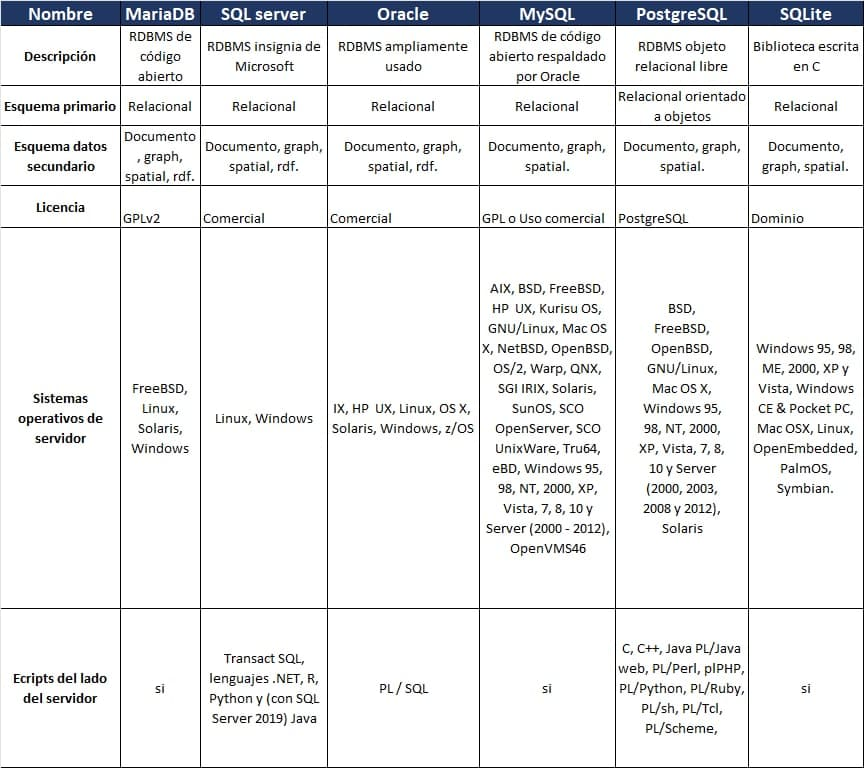
\includegraphics[width=0.90\textwidth]{Capitulo4/Img/GestionRnf/BaseDatos}
	\caption{Tabla comparativa de bases de datos relacionales}
	\label{fig:AGFDA}
\end{figure}
\subsubsection{Bases de datos no relacionales}

Ventajas de las bases de datos NoSQL. [22]
Este tipo de almacenamiento ofrece ciertas ventajas sobre los modelos SQL, tales como:
\begin{itemize}
	\item Se ejecutan en máquinas con pocos recursos: se pueden montar en máquinas con coste 
	reducido.
	\item Escalabilidad horizontal: si se necesita mejorar el rendimiento de la base de datos, este 
	se consigue al establecer más nodos en la red.
	\item Manejo de grandes volúmenes de datos: esto debido a que se usa una estructura 
	distribuida, en la mayoría de los casos con tablas hash
\end{itemize}


Razones para elegir NoSQL
\begin{itemize}
	\item 	Cuando el volumen de datos crece muy rápidamente en momentos puntuales, llegando a superar el terabyte de información.
	\item 	Cuando la escalabilidad de la solución relacionas no es viable tanto en costes como a nivel técnico.
	\item 	Cuando existen picos de uso del sistema por parte de los usuarios en múltiples veces.
	\item 		Cuando el esquema de datos no es homogéneo. 
\end{itemize}

Actualmente las bases de datos NoSQL más usadas son: Apache Cassandra, Redis, MongoDB, CouchDB y Hbase. [19]
\\

Algunas de sus características son las siguientes, ver Tabla \ref{tab:TBNOSQL}

  % Table generated by Excel2LaTeX from sheet 'Hoja20'
\begin{table}[H]
	\centering
	\caption{Tabla comparativa de bases de datos no relacionales}
\scalebox{0.65}{	\begin{tabular}{|p{7.145em}|p{5.355em}|p{5.355em}|p{5.355em}|p{5.355em}|p{5.355em}|}
		\toprule
		\rowcolor[rgb]{ .125,  .216,  .392} \textcolor[rgb]{ 1,  1,  1}{\textbf{Características}} & \textcolor[rgb]{ 1,  1,  1}{\textbf{MongoDB}} & \textcolor[rgb]{ 1,  1,  1}{\textbf{Cassandra}} & \textcolor[rgb]{ 1,  1,  1}{\textbf{CouchDB}} & \textcolor[rgb]{ 1,  1,  1}{\textbf{Hbase}} & \textcolor[rgb]{ 1,  1,  1}{\textbf{Redis}} \\
		\midrule
		\textbf{Lenguaje} & C++ & Java & Erlang & Java & C++ \\
		\midrule
		\textbf{Modelo de datos} & BSON & JSON & JSON & JSON & JSON \\
		\midrule
		\textbf{Tolerancia a fallas} & replicación  & replicación & replicación & Particionamiento y replicación & replicación \\
		\midrule
		\textbf{MapReduce } & Si & Si & Si & Si & Si \\
		\midrule
		\textbf{Modos de replicación} & Maestro esclavo & Maestro esclavo & Maestro esclavo & Maestro esclavo & Maestro esclavo \\
		\midrule
		\textbf{Protocolo } & TCP/IP & Thrift & HTTP/REST & Thrift, API & Similar a telnet \\
		\bottomrule
	\end{tabular}%
	\label{tab:TBNOSQL}}%
\end{table}%



\subsubsection{Tipo de base de datos elegida}

Con respecto a lo planteado a esta sección, a los requerimientos del sistema, así como las características de los conjuntos de datos, se optara por una implementación de \textbf{\textit{base de datos Relacional SQL}}, ya que el crecimiento de datos no es exponencial así mismo por los distintos tipos de clientes varios a tener, es mas productivo ajustar una base de datos a el tipo de requemamientos del cliente.


\subsection{Analista de proveedor de nube}\label{cap:azure}
En esta sección se describirán las características principales de los proveedores de nube, y sus diferencias entre sí.
La comparativa se llevara en puntos importantes, para el proyectos los cuales son: 
\begin{itemize}
	\item Tutoriales
	\item Documentación
	\item Interfaz grafica 
	\item Interfaz de terminal 
	\item Web APIs
	\item Soporte Open Sours 
	\item Soporte de proveedor 
\end{itemize}
Dichos datos son los mas importantes para poder generar la elección del proveedor de nueve, dicha comparativa se muestra en la tabla \ref{tab:cloudNuve}, [23],[24],[25],

  % Table generated by Excel2LaTeX from sheet 'Hoja21'
  % Table generated by Excel2LaTeX from sheet 'Hoja21'
\begin{table}[H]
	\centering
	\caption{Comparación entre proveedores de nube}
	\begin{tabular}{|p{10.715em}|c|p{5.355em}|p{5.355em}|}
		\toprule
		\rowcolor[rgb]{ .125,  .216,  .392} \textcolor[rgb]{ 1,  1,  1}{\textbf{Proveedor}} & \multicolumn{1}{p{5.355em}|}{\textcolor[rgb]{ 1,  1,  1}{\textbf{AWS}}} & \textcolor[rgb]{ 1,  1,  1}{\textbf{Azure}} & \textcolor[rgb]{ 1,  1,  1}{\textbf{Google Cloud}} \\
		\midrule
		\textbf{Video tutoriales} &   & OK & OK \\
		\midrule
		\textbf{Documentación} & \multicolumn{1}{p{5.355em}|}{OK } & OK & OK \\
		\midrule
		\textbf{Interfaz grafica} & \multicolumn{1}{p{5.355em}|}{OK } & OK & OK \\
		\midrule
		\textbf{Interfaz de línea de comandos } & \multicolumn{1}{p{5.355em}|}{OK } & OK & OK \\
		\midrule
		\textbf{Buen nivel de servicio} & \multicolumn{1}{p{5.355em}|}{OK } & OK & OK \\
		\midrule
		\textbf{Web APIs} & \multicolumn{1}{p{5.355em}|}{OK } & OK & OK \\
		\midrule
		\textbf{Soporte open source} &   & OK & OK \\
		\midrule
		\textbf{Experiencia con Cloud } &   & OK  & OK  \\
		\bottomrule
	\end{tabular}%
	\label{tab:cloudNuve}%
\end{table}%
Como se observa en la tabla la opción más viable para este sistema, de acuerdo con las características ofrecidas por cada proveedor de servicios de nube, es Microsoft Azure. 


\subsection{Análisis de marcos de trabajo de desarrollo web}

El análisis de los marcos de trabajo se realizará a través de dos ejes, el Front End y el Back End.
\subsubsection{Análisis de Front End}\label{cap:frontend}
De acuerdo con las tendencias actuales, los principales marcos de trabajo para Front End son  angular, vue y  react , por tanto, se consideraron únicamente dichos marcos de trabajo para su análisis, dicho análisis se basaran en los siguientes puntos: [26],[27],[28]
\begin{itemize}
	\item Rendimiento
	\item Documentación
	\item Curva de aprendizaje
	\item Lenguaje Base
\end{itemize}
Teniendo los puntos de comparación, se presenta la siguiente tabla \ref{tab:TABLAFRONEND}. 
  % Table generated by Excel2LaTeX from sheet 'Hoja22'
\begin{table}[H]
	\centering
	\caption{Comparativo de marcos de trabajo para Front End }
\scalebox{0.60}{
	\begin{tabular}{|p{9.645em}|p{15.855em}|p{14.355em}|p{16.285em}|}
		\toprule
		\rowcolor[rgb]{ .125,  .216,  .392} \textcolor[rgb]{ 1,  1,  1}{\textbf{Marco de trabajo}} & \textcolor[rgb]{ 1,  1,  1}{\textbf{Angular}} & \textcolor[rgb]{ 1,  1,  1}{\textbf{Vue}} & \textcolor[rgb]{ 1,  1,  1}{\textbf{React}} \\
		\midrule
		\textbf{Rendimiento} & No es tan rápido como React, pero es debido a que cuenta con un enlace de datos bidireccional  & Comparte con Angular el DOM virtual, los componentes reactivos y componibles lo hacen tan rápido como Angular. & Es la opción más rápida disponible debido a que es sólo una biblioteca orientada al DOM y el enlace unidireccional. \\
		\midrule
		\textbf{Documentación} & Una de las mejores documentaciones, debido a que es simple, corta y al punto.  & Debido a su sencillez, la documentación oficial es suficiente para empezar a trabajar. & Debido a su flexibilidad, es difícil encontrar la documentación exacta puede resultar complicado. \\
		\midrule
		\textbf{Curva de aprendizaje} & Su curva es más pronunciada en comparación a otros marcos, debido a que la documentación es extremadamente grande y requiere familiarización con algunos conceptos antes de trabajar. & Su curva es la menos pronunciada, debido a que sólo se necesita conceptos básicos de HTML, CSS y JS. Se puede crear aplicaciones simples y no triviales en menos de un día. & Su curva no es tan pronunciada gracias a que es una biblioteca básica con pocas API y flujos de trabajo. Se puede utilizar con mayor facilidad.  \\
		\midrule
		\textbf{Sostenibilidad} & Desarrollo orientado a componentes & Desarrollo orientado a componentes & Desarrollo orientado a componentes \\
		\midrule
		\textbf{Lenguaje Base} & TypeScript & JavaScript & JavaScript \\
		\bottomrule
	\end{tabular}%
	\label{tab:TABLAFRONEND}}%
\end{table}%

Con respecto al análisis realizado en la tabla \ref {tab:TABLAFRONEND}, se considera como marco de trabajo para el desarrollo del Front end el lenguaje Java Scrip con su Framework Angular.
\subsubsection{Analisis de Back End}\label{cap:backend}
De acuerdo ala implementacion de en aplicaciones web, los principales marcos de trabajo para el Back End, son:  Laravel, Flask, Spring Boot, y ASP. NET CORE por tanto, se consideran estos mismos para la comparativa que se muestra en la tabla \ref {tab:FRONTENDCOM}, [29],[30],[31].


\begin{table}[H]
	\centering
	\caption{Comparación de marcos de trabajo para Back End }
\scalebox{0.60}{	\begin{tabular}{|p{6.93em}|p{10em}|p{10em}|p{10em}|p{10em}|}
		\toprule
		\rowcolor[rgb]{ .125,  .216,  .392} \textcolor[rgb]{ 1,  1,  1}{\textbf{Marco de trabajo}} & \textcolor[rgb]{ 1,  1,  1}{\textbf{Laravel}} & \textcolor[rgb]{ 1,  1,  1}{\textbf{Flask}} & \textcolor[rgb]{ 1,  1,  1}{\textbf{Spring Boot}} & \textcolor[rgb]{ 1,  1,  1}{\textbf{ASP. Net Core}} \\
		\midrule
		\textbf{Comunidad} & Tiene una amplia comunidad debido a que PHP domina el 79\% del mercado en lo que respecta a la programación del lado de servidor. & Su comunidad no es tan amplia debido a que es un marco relativamente nuevo.  & Es el marco más popular de Java, debido a su velocidad, simplicidad y productividad.\newline{}Respaldada por comunidad de código abierto & Amplia comunidad debido a su versatilidad para realizar aplicaciones web. \\
		\midrule
		\textbf{Rendimiento} & Ofrece buen rendimiento debido a que aprovecha las virtudes de la memoria cache. & Fue diseñado para proveer alto rendimiento para la mayoría de los usuarios, debido a que tiene pocas capas de abstracción.  & Su rendimiento es regular en comparación a otros marcos, sus virtudes no se centran en el rendimiento. & Su mayor ventaja respecto a otros marcos es el rendimiento, debido a que recibe continuamente actualizaciones. \\
		\midrule
		\textbf{Documentación} & Amplia documentación y comunidad debido a su dominio del mercado. & Gracias a su sencillez, la documentación oficial es suficiente para empezar a desarrollar aplicaciones. & Amplia documentación y comunidad debido a su amplio uso en la industria. & Cuenta con la documentación más amplia y precisa, pues esta es provista por Microsoft. \\
		\midrule
		\textbf{Curva de aprendizaje} & Curva de aprendizaje regular gracias a que PHP es un lenguaje sencillo y no requiere conocimientos previos. & Tiene la curva de aprendizaje menos pronunciada, debido a que es un marco minimalista y su orientación es al desarrollo acelerado.  & Curva de aprendizaje más pronunciada en comparación de los otros marcos, debido su filosofía de convención sobre configuración. & Curva de aprendizaje menos pronunciada debido a que no requiere tanto código. \\
		\midrule
		\textbf{Mantenibilidad} & Desarrollo orientado a módulos. & Desarrollo orientado a módulos. & Desarrollo orientado a Módulos. & Desarrollo orientado a Módulos. \\
		\midrule
		\textbf{Lenguaje Base} & PHP & Python & Java & C\# \\
		\bottomrule
	\end{tabular}%
	\label{tab:FRONTENDCOM}}%
\end{table}%
De acuerdo a el análisis realizado en la tabla \ref{tab:FRONTENDCOM} entre marcos de trabajo para el Back End, se seleccionó \textbf{\textit{Spring Boot}} como marco de trabajo, pues pese a su curva de aprendizaje más pronunciada y su rendimiento regular, ofrece la mejor compatibilidad con micro servicios.
\newpage

\section{Requerimientos funcionales}


En la siguiente siguiente sección se describirá el análisis de los requerimientos funcionales que formaran parte del sistema desarrollado, los cuales son: 

\begin{itemize}
	\item Vista general del sistema. 
	\item Módulo de Registro y levantamiento de incidentes.
	\item Modulo de Gestiona y cierre de incidentes
	\item Modulo de Gestión de Activos
	\item Modulo de Gestión de informes
	\item Modulo de Gestión de usuarios del sistema
\end{itemize}



\newpage
\subsection{Vista general del sistema}
En el siguiente diagrama de clases de usos se describe la interacción general del sistema, como se muestra en la figura \ref{fig:DCUG}.

\begin{figure}[h]
	\centering
	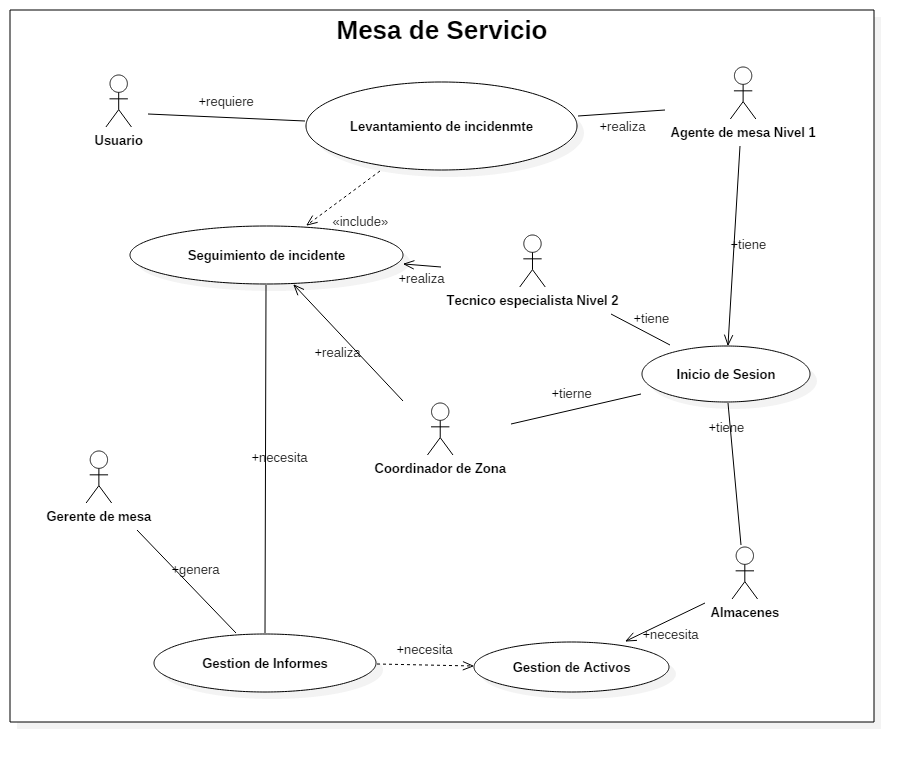
\includegraphics[width=1.1\textwidth]{Capitulo4/Img/Mesa2}
	\caption{Diagrama de clases General del sistema"}
	\label{fig:DCUG}
\end{figure}


El diagrama anteriormente mencionado, contiene los casos de usos que se desarrollaran como módulos en el sistema, por lo cual la descripción de cada caso de uso se realiza en el análisis del modulo correspondiente. 

\subsection{Modulo de registro y levantamiento de incidentes}
El módulo de registro y levantamiento de incidentes tiene como objetivo recabar información, categorizar y registrar el incidente que sea solicitado por algún usuario pertenecientes a las cuentas/clientes.


\subsubsection{Descripción de caso de uso "Levantamiento de incidente".}
El siguiente análisis se realiza con los requerimientos necesarios para la correcta operación del modulo.

\begin{multicols}{2}
\textbf{Caso de uso: Levantamiento de Incidente.}

\begin{itemize}
	\item[$*$]  Actor principal
	\begin{itemize}
		\item Agentes de la mesa de servicio (Nivel 1)
	\end{itemize}
	\item[$*$]  Objetivo en contexto
		\begin{itemize}
		\item Recibir y registrar los incidentes solicitados por los usuarios, todo por medio del software de mesa de servicio.
	\end{itemize}
	\item[$*$]  Precondiciones
\begin{itemize}
	\item El usuario solicitante de la atención necesariamente deberá pertenecer a alguna Dependencia cliente registrada. 
	\item La incidencia solo aplicara a las atenciones descritas en el catálogo de servicio.
	\item El agente de mesa de servicio requiere estar autentificado en el sistema.
\end{itemize}	
	\item[$*$]  Disparador
\begin{itemize}
	\item Un usuario perteneciente a alguna dependencia cliente, realiza una llamada o envía un correo a mesa de servicio expresando alguna falla. 
\end{itemize}
	\item[$*$]  Escenario
	\begin{itemize}
		\item El Agentes de la mesa de servicio (Nivel 1) introduce su identificación de usuario,
		\item El sistema despliega todos los botones de las funciones principales.
		\item El Agentes de la mesa de servicio (Nivel 1) selecciona “Nuevo Ticket” entre los botones de funciones principales.
		\item El sistema despliega toda la interfaz para el levantamiento de Tickets.
		\item El Agentes de la mesa de servicio (Nivel 1) categoriza si es un Incidente o Requerimiento 
		\item El Agentes de la mesa de servicio (Nivel 1) captura los datos del usuario 
		\item El Agentes de la mesa de servicio (Nivel 1) captura los datos del equipo de computo 
		\item El Agentes de la mesa de servicio (Nivel 1) asigna el nivel de SLA, y la asignación del personal de mesa de servicio para su seguimiento y atención. 
	\end{itemize}
	\item[$*$]  Excepciones
	\begin{itemize}
		\item No se dispone de mas atenciones que no se estén especificadas en el catalogo de servicios. 
		\item El sistema no esta programado para tener tikets masivos. 
		\item No se puede generar un ticket con más de 2 fallas de equipos distintos.	
	\end{itemize}
	\item[$*$]  Prioridad
	\begin{itemize}
		\item De alta prioridad, es la función de inicio del proceso del sistema.
	\end{itemize}
	\item[$*$]  Frecuencia de Uso
\begin{itemize}
	\item Frecuencia alta
\end{itemize}
	\item[$*$]   Canal al actor.
\begin{itemize}
	\item 	A través de un navegador con base en PC o LAPTOP y conexión a internet.
\end{itemize}
	\item[$*$]  Actores secundarios
\begin{itemize}
	\item Usuario -cliente
\end{itemize}
\end{itemize}

\end{multicols}



\subsubsection{Requerimientos del módulo de registro y levantamiento de incidentes}\label{Mod:RQLDI}%
Para el correcto desarrollo del modulo \ref{Mod:RQLDI}, se generan los requemamientos fundamentales para el funcionamiento de este mismo, siendo así descritos en la tabla \ref{tab:addlabel}.

  % Table generated by Excel2LaTeX from sheet 'Hoja3'
\begin{table}[H]
	\centering
	\caption{Requerimientos funciones del modulo-registro y levantamiento de incidentes }
	\begin{tabular}{|l|l|}
		\toprule
		\rowcolor[rgb]{ .125,  .216,  .392} \multicolumn{1}{|p{12.5em}|}{\textcolor[rgb]{ 1,  1,  1}{\textbf{Requerimiento}}} & \multicolumn{1}{p{24.285em}|}{\textcolor[rgb]{ 1,  1,  1}{\textbf{Descripción}}} \\
		\midrule
		\multicolumn{1}{|p{12.5em}|}{R1} & \multicolumn{1}{p{24.285em}|}{Recepción de reporte de Incidente} \\
		\midrule
		\multicolumn{1}{|p{12.5em}|}{R2} & \multicolumn{1}{p{24.285em}|}{Validación de información del usuario} \\
		\midrule
		\multicolumn{1}{|p{12.5em}|}{R3} & \multicolumn{1}{p{24.285em}|}{Validación de la información del equipo de computo} \\
		\midrule
		\multicolumn{1}{|p{12.5em}|}{R4} & \multicolumn{1}{p{24.285em}|}{Categorizar el servicio.} \\
		\midrule
		R5 & Escalamiento de incidente. \\
		\bottomrule
	\end{tabular}%
	\label{tab:addlabel}%
\end{table}%
\subsubsection{Actividades del proceso de Registro y levantamiento de incidentes}
A continuación, se detallan las actividades, entradas y salidas de los procesos de "Registro y levantamiento de incidentes”, como se muestra en la tabla \ref{tab:FDTLDI} 


  % Table generated by Excel2LaTeX from sheet 'Hoja4'
\begin{table}[H]
	\centering
	\caption{Flujo de trabajo, levantamiento y registro de incidentes}
	\scalebox{0.55}{ \begin{tabular}{|c|p{9.5em}|p{22em}|p{14.645em}|}
	\toprule
	\rowcolor[rgb]{ .184,  .329,  .588} \multicolumn{4}{|p{51.5em}|}{\textcolor[rgb]{ 1,  1,  1}{Levantamiento y registro de incidencias}} \\
	\midrule
	\rowcolor[rgb]{ .184,  .329,  .588} \multicolumn{1}{|p{5.355em}|}{\textcolor[rgb]{ 1,  1,  1}{ID}} & \textcolor[rgb]{ 1,  1,  1}{Actividad} & \textcolor[rgb]{ 1,  1,  1}{Descripción} & \textcolor[rgb]{ 1,  1,  1}{Responsable} \\
	\midrule
	1 & Identifica incidente. & Usuario en dependencia o  corporativo detecta incidente disruptivo en su equipo de cómputo. & Usuario  \\
	\midrule
	2 & Reporta incidente a mesa de servicio. & Reporta el incidente a mesa de servicio mediante correo electrónico o llamada telefónica. & Usuario  \\
	\midrule
	3 & Recibe reporte deincidencia. & Recibe información del usuario. & Agente de Mesa de Servicio  \\
	\midrule
	4 & Revisa que la información sea completa. & Revisa que la información del incidente sea completa:\newline{}•	Operación del error \newline{}•	Datos del usuario afectado.\newline{}1.	Nombre \newline{}2.	Correo \newline{}3.	Teléfono \newline{}4.	Extensión \newline{}5.	Piso\newline{}6.	Área   \newline{}7.	Ubicación\newline{}8.	-Adscripción\newline{}•	Dependencia \newline{}•	Datos del equipo de computo \newline{}1.	Service tag \newline{}2.	Marca\newline{}3.	Modelo \newline{}4.	Numero de Serie \newline{}5.	Tipo de equipo \newline{}Nota: Si la información está completa se continúa en la actividad 6, en caso contrario continúa en la actividad 5 & Agente de Mesa de Servicio \\
	\midrule
	5 & Solicita información adicional del incidente. & Solicita por correo electrónico o llamada la información adicional para poder atender el incidente.	\newline{}Agente de Mesa de Servicio & Agente de Mesa de Servicio \\
	\midrule
	6 & Categoriza incidente. & Categoriza el incidente, es decir, define si es incidente técnico o requerimiento.\newline{}Nota: Si la solicitud es de tipo requerimiento,  se programa la atención con la atención usuario Y se registra el requerimientos. & Agente de Mesa de Servicio \\
	\midrule
	7 & Categorización de SLA  & Categoriza el SLA dependiendo el nivel de impacto a la operación del usuario. Descrita en la matriz de impacto.  & Agente de Mesa de Servicio \\
	\midrule
	8 & Asigancion de atencion  &  Asignacion un responsable miembro de la mesa de servicio para ell seguimiento  de solicitud del incidente, como se estable en tabla de escalmiento de incidentes. & Agente de Mesa de Servicio \\
	\midrule
	9 & Registra el incidente & Registra en la herramienta Service Manager el incidente reportado y notifica el inicio de la atención de este. & Agente de Mesa de Servicio \\
	\bottomrule
	
	\end{tabular}%
	\label{tab:FDTLDI}}%
\end{table}%


\subsubsection{Diagrama de secuencia - Registro y levantamiento de incidentes}

En el siguiente figura  \ref{fig:DSLDI} se representa la descripción de los procesos antes mencionados en la Tabla \ref{tab:FDTLDI}, basada en un modelo de  diagrama de secuencia, donde los actores participantes se limitan solo a dos, usuario y agente de mesa de servicio. 

\begin{figure}[H]
	\centering
	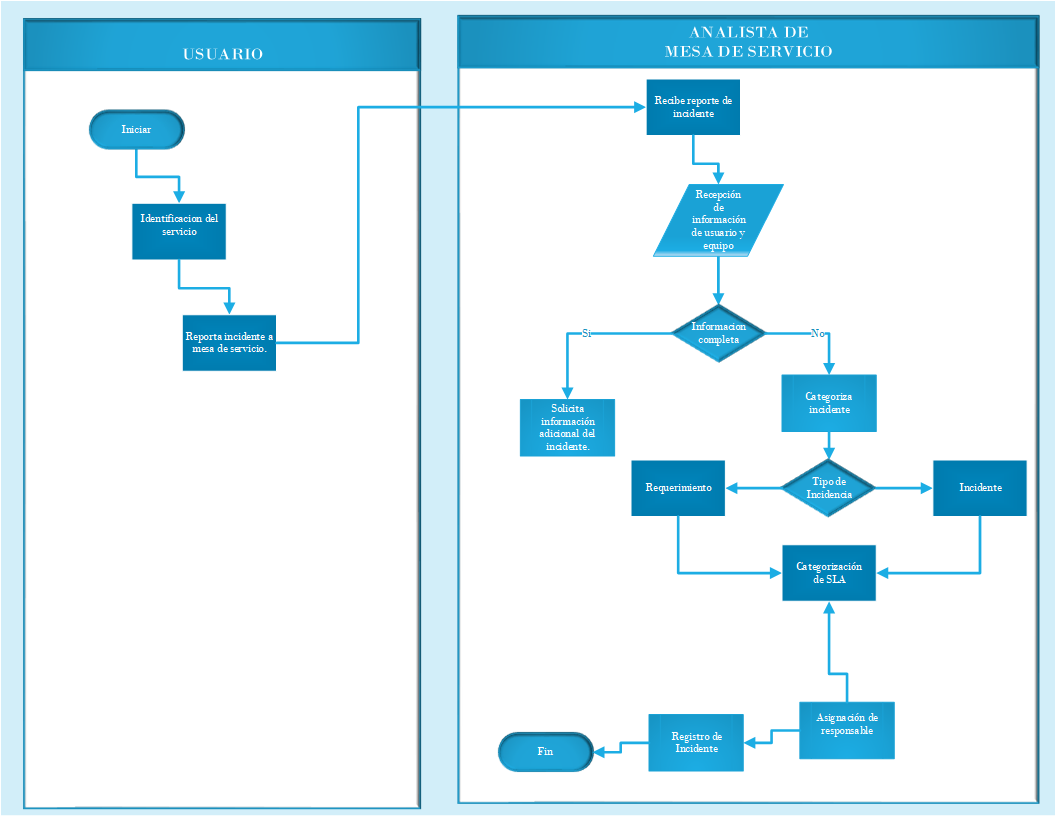
\includegraphics[width=0.9\textwidth]{Capitulo4/Img/Regitro_de_Incidente}
	\caption{Diagrama de secuencia - "Registro y levantamiento de incidentes"}
	\label{fig:DSLDI}
\end{figure}

\subsubsection{Interfaz de Grafica - Levantamiento de incidentes}
 En la figura \ref{fig:IF} podemos visualizar el home del usuario llamado Agente de mesa de servicio SOPORTE NIVEL 1, el cual realizara el levantamiento de incidente. Dicho levantamiento lo ara, dando click en la parte superior derecha en el botón de "Nuevo INC".
 
 \begin{figure}[H]
 	\centering
 	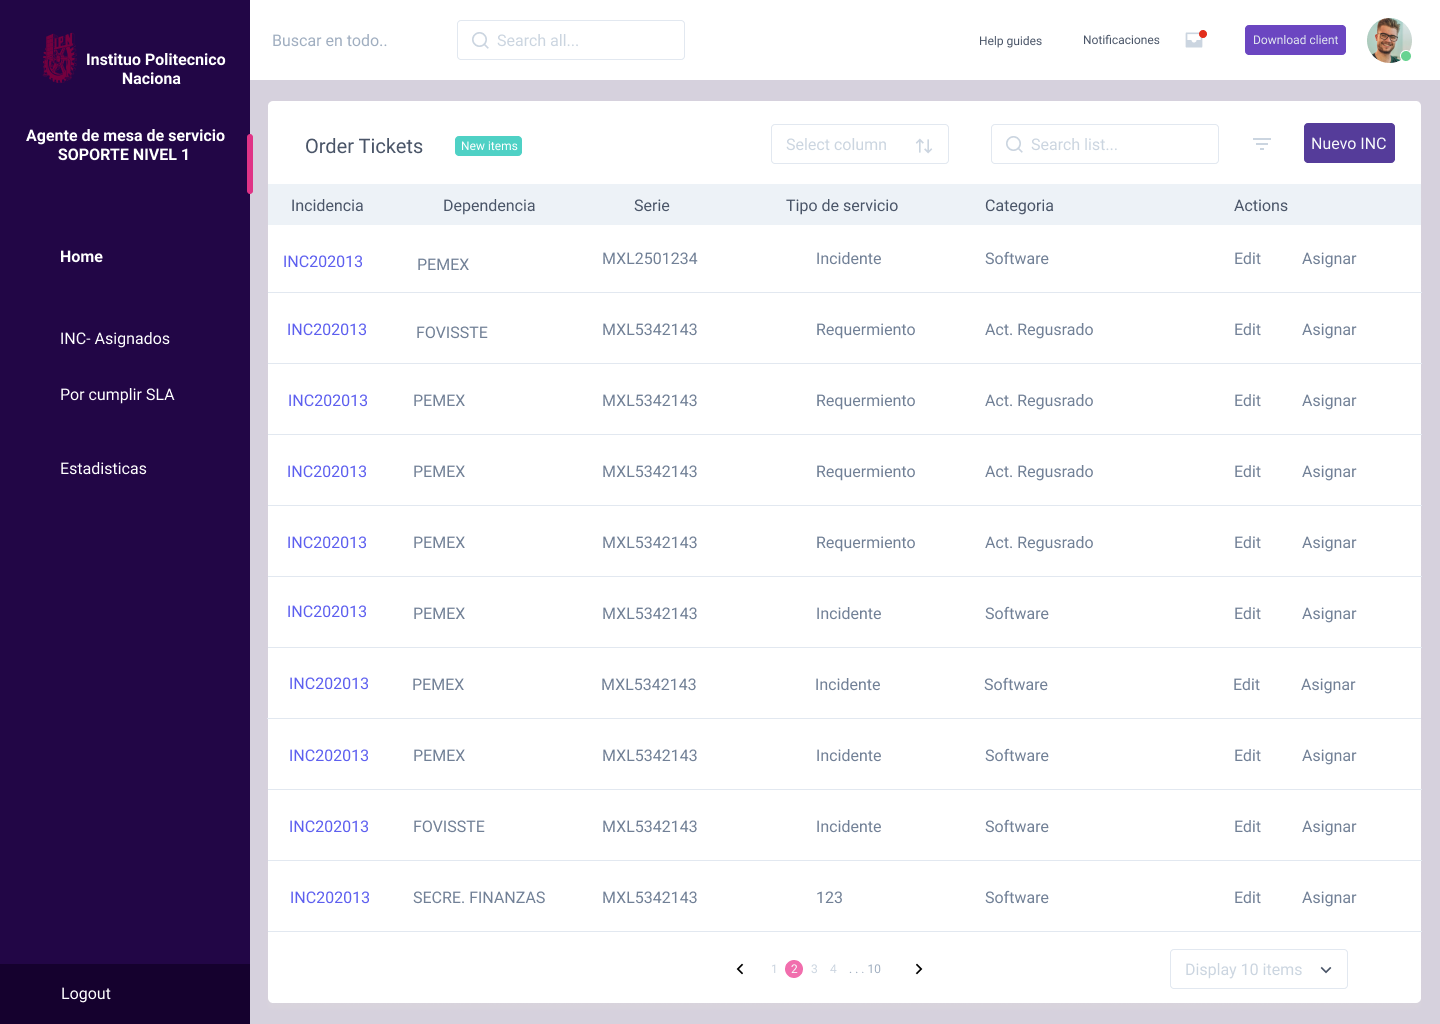
\includegraphics[width=1.1\textwidth]{Capitulo4/Img/Levantamiento_inc/home}
 	\caption{Interfaz Home- Levantamiento de incidentes"}
 	\label{fig:IF}
 \end{figure}
A continuación se  mostrara la siguiente interfaz figura \ref{fig:IFHLDI}, donde se capturan todos los datos del Incidente o Requerimiento. 
\begin{figure}[H]
	\centering
	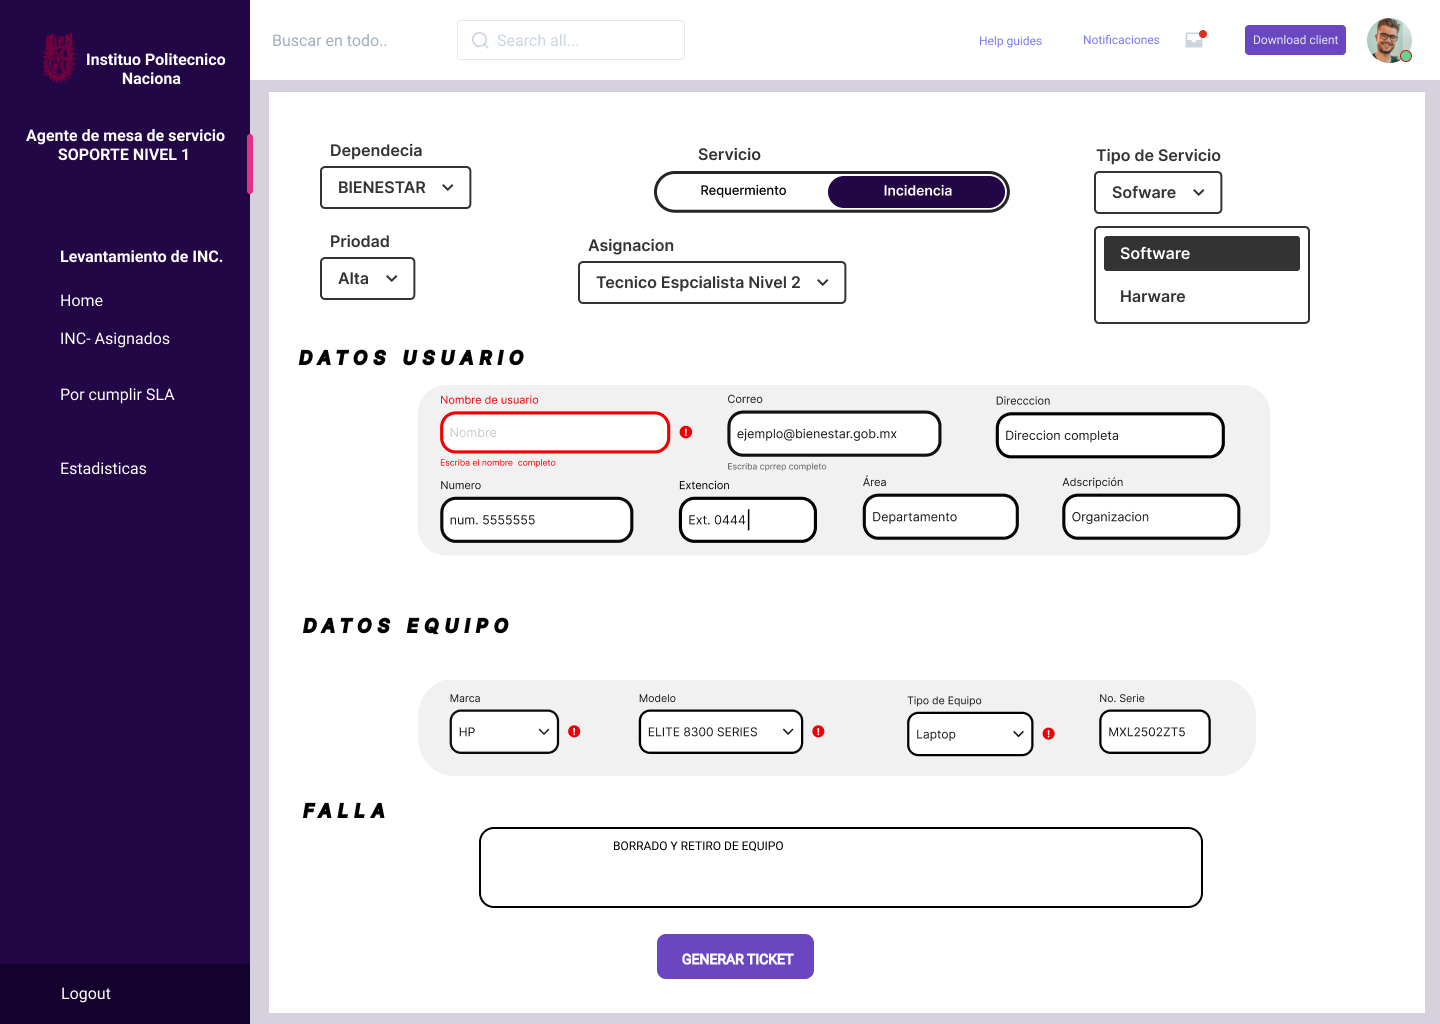
\includegraphics[width=1.1\textwidth]{Capitulo4/Img/Levantamiento_inc/Registro}
	\caption{Interfaz Levantamiento de incidentes"}
	\label{fig:IFHLDI}
\end{figure}
 



\newpage
\subsection{Modulo de Gestión  y cierre de incidentes}
El módulo de gestión de incidentes tiene como objetivo dar el seguimiento del ticket hasta el cierre, por lo cual tendrá como funciones principales, documentar las acciones  realizadas para generar una solución al Ticket generado. 
\subsubsection{Requerimientos del módulo Gestiona y cierre de incidentes}\label{Mod:RQMGI}


Para el correcto desarrollo del modulo \ref{Mod:RQMGI}, se generan los requemamientos fundamentales para el funcionamiento de este mismo, siendo así descritos en la tabla \ref{tab:RQMGDS}.


  % Table generated by Excel2LaTeX from sheet 'Hoja9'
\begin{table}[H]
	\centering
	\caption{Requerimientos funciones del modulo- Gestión de incidentes}
\scalebox{0.90}{	\begin{tabular}{|p{9.145em}|l|}
		\toprule
		\rowcolor[rgb]{ .125,  .216,  .392} \textcolor[rgb]{ 1,  1,  1}{\textbf{Requerimiento}} & \multicolumn{1}{p{24.285em}|}{\textcolor[rgb]{ 1,  1,  1}{\textbf{Descripción}}} \\
		\midrule
		R6 & \multicolumn{1}{p{24.285em}|}{Soporte a gestión de incidentes.} \\
		\midrule
		R7 & \multicolumn{1}{p{24.285em}|}{Soporte primera instancia o instancia cero.} \\
		\midrule
		R8 & \multicolumn{1}{p{24.285em}|}{Monitoreo del incidente.} \\
		\midrule
		R9 & \multicolumn{1}{p{24.285em}|}{Solución y prueba.} \\
		\midrule
		R10 & Cierre de la Incidencia \\
		\bottomrule
	\end{tabular}%
	\label{tab:RQMGDS}}%
\end{table}%
\textbf{}





\subsubsection{Descripción de caso de uso Gestiona y cierre de incidentes}



El siguiente análisis se realiza con los requemamientos necesarios para la correcta operación del modulo.

\begin{multicols}{2}

	\textbf{Caso de uso: Gestión de incidentes.}
	\begin{itemize}
		\item[$*$]  Actor principal
		\begin{itemize}
			\item Coordinador de zona (Nivel 2)
		\end{itemize}
		\item[$*$]  Objetivo en contexto
		\begin{itemize}
			\item Se le debe de dar seguimiento a los incidentes reportados de principio a fin.
			\item Documentar las observaciones o soluciones que se van realizando en el proceso de solución.
			\item Realizar la investigación de las posibles soluciones de corrección y dar el diagnostico de las causas.
		\end{itemize}
		\item[$*$]  Precondiciones
		\begin{itemize}
			\item Solo se atenderán tickes registrados en la herramienta de mesa de servicio
			\item El coordinador de zona Nivel 2 requiere estar autentificado en el sistema.
			
		\end{itemize}	
		\item[$*$]  Disparador
		\begin{itemize}
			\item Agente de mesa de servicio Nivel 1, registra un incidente en el sistema de mesa de servicio 
		\end{itemize}
		\item[$*$]  Escenario
		\begin{itemize}
			\item El Agentes de la mesa de servicio (Nivel 1), realiza la el primer diagnostico 
			\item Primero diagnostico se documenta en la herramienta de mesa de servicio.
			\item El Agentes de la mesa de servicio (Nivel 1, reasigna a un coordinador de zona, si el problema no es solucionable a primer nivel. 
			\item El coordinador de zona (Nivel 2) asigna la incidencia a un técnico especializado Nivel 2, correspondiente a la zona de atención. 
			\item El técnico especialista (Nivel 2) realiza el segundo diagnostico 
			\item El técnico especialista (Nivel 2) notifica y documenta en la herramienta de mesa de servicio la solución.
			\item El coordinador de zona (Nivel 2), gestiona y valida el VoBo del usuario sobre la atención. 
			
		\end{itemize}
		\item[$*$]  Excepciones
		\begin{itemize}
			\item El coordinar de zona y agente de mesa de servicio, no pueden gestionar un mismo incidente. 		
		\end{itemize}
		\item[$*$]  Prioridad
		\begin{itemize}
			\item La prioridad asignada será con base a la fluctuación del Nivel de SLA asignado.
		\end{itemize}
		\item[$*$]  Frecuencia de Uso
		\begin{itemize}
			\item Frecuencia alta
		\end{itemize}
		\item[$*$]   Canal al actor.
		\begin{itemize}
			\item 	A través de un navegador con base en PC o LAPTOP y conexión a internet.
		\end{itemize}
		\item[$*$]  Actores secundarios
		\begin{itemize}
			\item Agente de mesa servicio 
			\item Técnico especialista nivel 2
			\item Usuario, saltante del servicio
			
		\end{itemize}
	\end{itemize}
	
\end{multicols}



\subsubsection{Actividades del proceso de Gestiona y cierre de incidentes}

A continuación, se detallan las actividades, entradas y salidas de los procesos de gestiona de incidentes”, como se muestra en la tabla \ref{tab:FDTGDI} 


\begin{table}[H]
	\centering
	\caption{Flujo de trabajo - Gestión de incidentes }
	\scalebox{0.40}{ \begin{tabular}{|c|p{12.855em}|p{42.43em}|p{7.645em}|}
			\toprule
			\rowcolor[rgb]{ .188,  .329,  .588} \multicolumn{4}{|p{68.285em}|}{\textcolor[rgb]{ 1,  1,  1}{\textbf{Gestion de Incidentes }}} \\
			\midrule
			\rowcolor[rgb]{ .188,  .329,  .588} \multicolumn{1}{|p{5.355em}|}{\textcolor[rgb]{ 1,  1,  1}{\textbf{ID}}} & \textcolor[rgb]{ 1,  1,  1}{\textbf{Actividad}} & \textcolor[rgb]{ 1,  1,  1}{\textbf{Descripción}} & \textcolor[rgb]{ 1,  1,  1}{\textbf{Responsable}} \\
			\midrule
			
			1 & \multicolumn{1}{c|}{Levantamiento de incidente } & Registra reporte en herramienta Mesa de servicio asignando plantilla, datos usuario, datos equipos,área, impacto, prioridad, urgencia y una descripción del diagnóstico. & Agentes de la mesa de servicio (Nivel 1) \\
			\midrule
			2 & \multicolumn{1}{c|}{Diagnóstico inicial.} & Confirma si se trata de una incidencia de tipo software.  En caso de que el erro se encuentre en la Base de conocimientos del sistema  se atenderá con respecto a la información que se encuentre en dicha B.D, así mismo se determina si cuenta con  los elementos necesarios para resolver  y determina tiempo de resolución de acuerdo  con la Matriz de urgencia e impacto.\newline{}\newline{}\newline{}Nota:\newline{}-	en caso de conocer y haber resuelto el erro pasar a actividad 7.\newline{}-	si se trata de un error técnico (Hardware)  o Requerimiento de cualquier tipo pasar a la actividad 3.\newline{}\newline{}\newline{} & Agentes de la mesa de servicio (Nivel 1) \\
			\midrule
			3 & \multicolumn{1}{c|}{Escalamiento Incidente } & El escalamiento se llevara acabo cuando el servicio solicitado se  encuentre entre error técnico (Hardware)  o Requerimiento de cualquier tipo, \newline{}dicho escalamiento se ara al coordinador de zona (Nivel 2) al cual corresponda la zona de atención del ticket. \newline{}\newline{}Dicha acción se documentara en la herramienta de mesa de servicio. & Agentes de la mesa de servicio (Nivel 1) \\
			\midrule
			4 & \multicolumn{1}{c|}{Asignación a Técnico } & La asignación de la incidencia se ara al técnico especializado que se encuentre en la zona de atención.  & Coordinador de Zona (Nivel 2) \\
			\midrule
			5 & \multicolumn{1}{c|}{Diagnóstico segundo Nivel .} & Confirma si se trata de una incidencia de tipo software. \newline{}En caso de que el erro se encuentre en la Base de conocimientos del sistema \newline{}se atenderá con respecto a la información que se encuentre en dicha B.D.\newline{}\newline{}\newline{}Notas:\newline{}\newline{}- 	En caso de que se requiera alguna pieza de Hardware pasar a la actividad 6.\newline{}-             En caso de que el servicio sea un requerimiento de tipo implementación pasar a actividad 7 \newline{}-	En caso de conocer el error pasar a actividad 8. &  Técnico Especialista Nivel 2 \\
			\midrule
			6 & \multicolumn{1}{c|}{Solicitud de refacción } & El técnico especialista  solicitada a almacenes una refacción del Hardware dañado\newline{}Este proceso, lo documentara en la herramienta mesa de servicio  &  Tecnico Especialista Nivel 2 \\
			\midrule
			7 & Atención requerimiento tipo implementación  & El tecnico especialista valida si se encuentra en sitio el equipo a implementar si es contrario, el ticket se mantiene en estatus de proceso. \newline{}\newline{}Este proceso se documenta en la herramienta de mesa de servicio &  Técnico Especialista Nivel 2 \\
			\midrule
			8 & Notifica resolución a mesa de servicio. & Notifica a coordinador de mesa de servicio que el incidente ha sido resuelto. &  Técnico Especialista Nivel 2 \\
			\midrule
			9 & Solicita validación con el usuario & Solicita al usuario la validación sobre el servicio, dicha validación se ara por via correo electrónico.\newline{}\newline{}Nota:\newline{}- Si la validacion no es pocitiva pasar a la activas 2 o 5 según sea el caso  & Coordinador de Zona (Nivel 2) /\newline{}Agentes de la mesa de servicio (Nivel 1) \\
			\midrule
			10 & Cierre de Ticket  & Se documenta la soluciona, asi mismo se adjunta el correo de validación del usuario. & Coordinador de Zona (Nivel 2) /\newline{}Agentes de la mesa de servicio (Nivel 1) \\
			\bottomrule
		\end{tabular}%
		\label{tab:FDTGDI}}%
\end{table}%


\subsubsection{Diagrama de secuencia - Gestiona y cierre de incidentes}




En el siguiente diagrama \ref{} de secuencias se describe las actividades realizadas por los distintos actores en el módulo de gestión de incidentes, así mismo se incluye un nuevo módulo que se describirá en las siguientes secciones llama “Modulo de gestión de activos”, este inicio se identifica con un círculo verde. 


\begin{figure}[H]
	\centering
	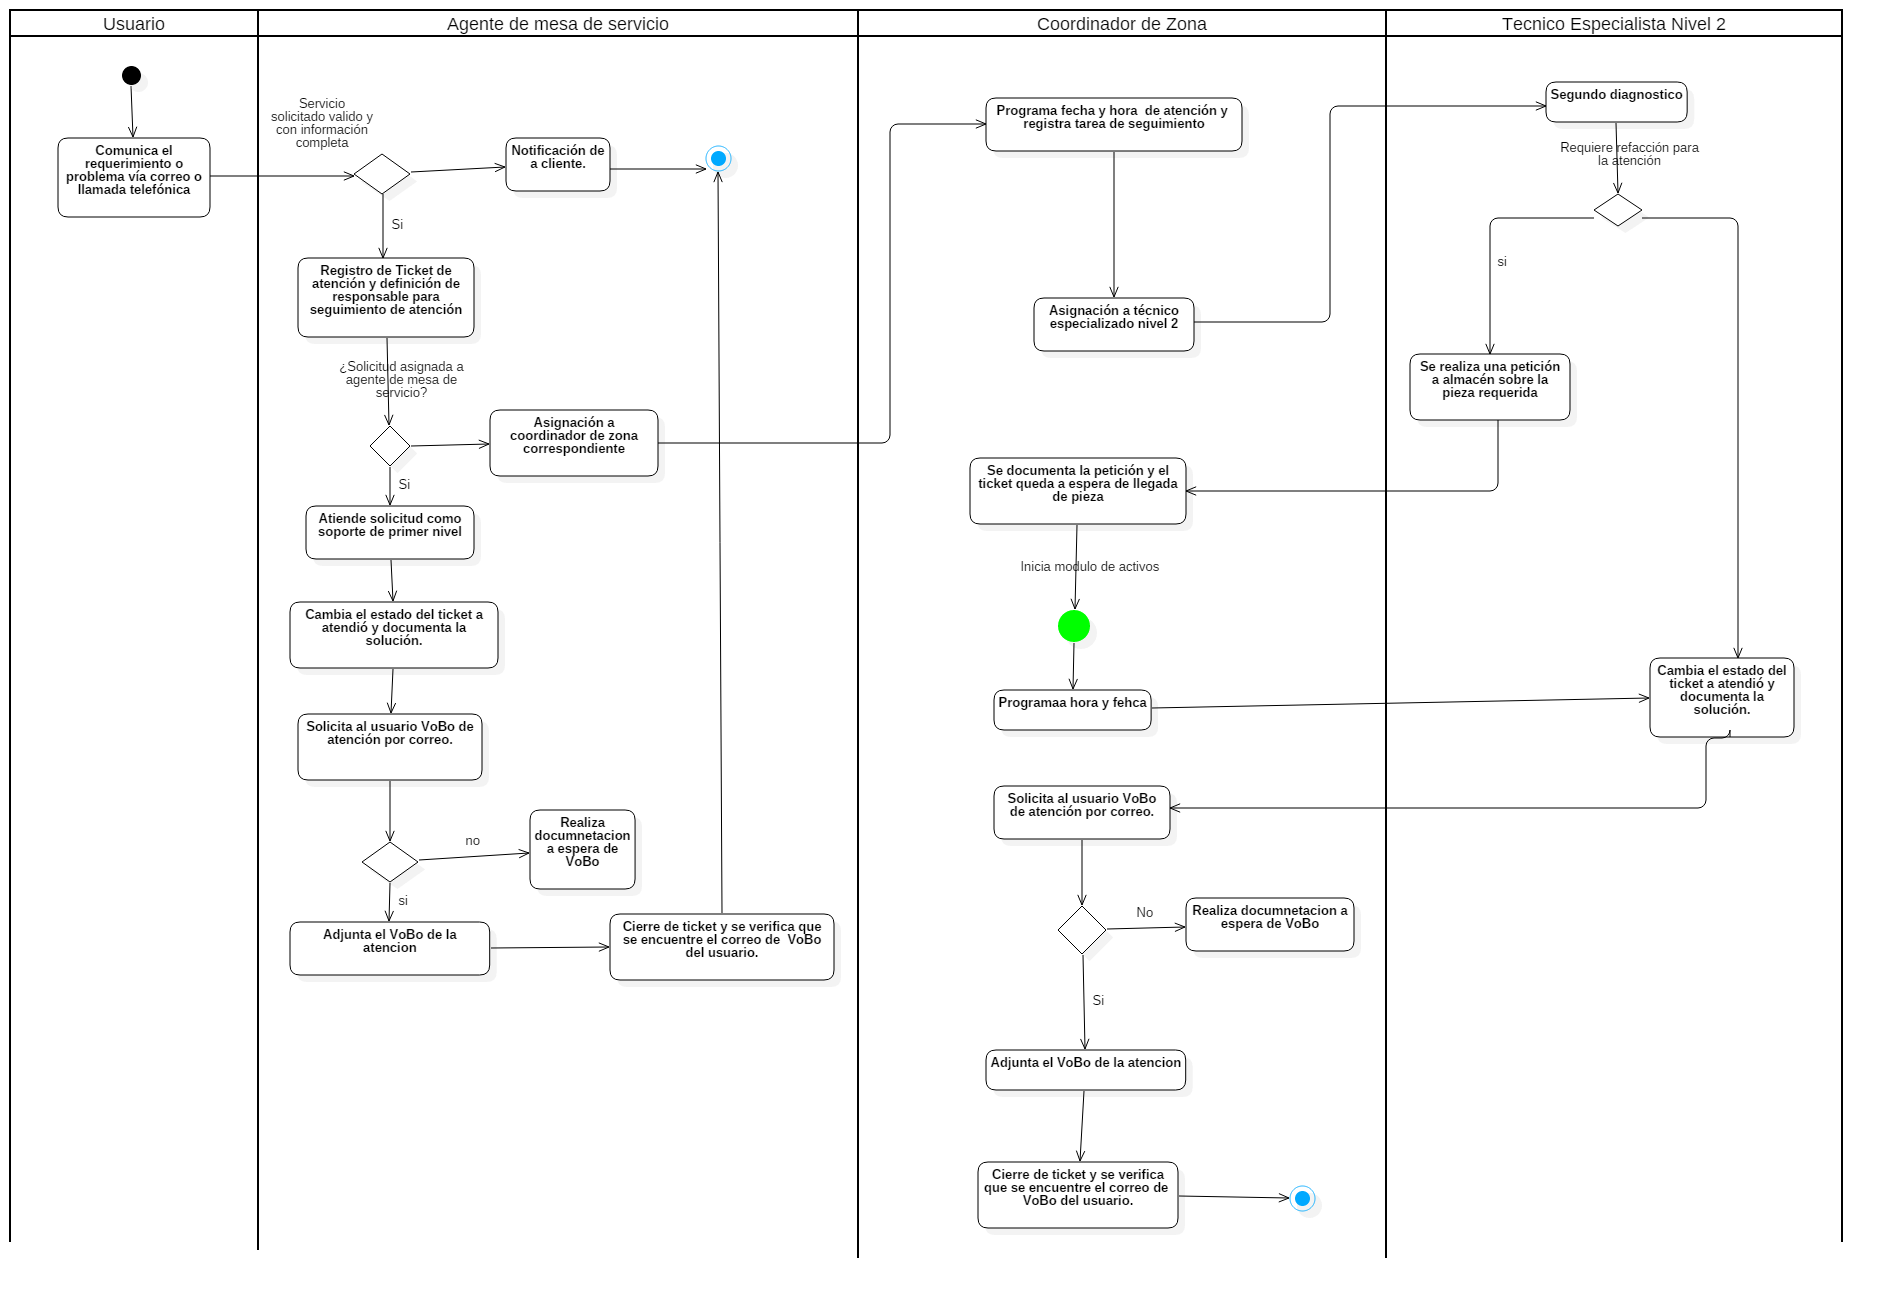
\includegraphics[width=0.9\textwidth]{Capitulo4/Img/GestionInc/GestionINC}
	\caption{Diagrama de secuencia - "Gestiona y cierre de incidentes"}
	\label{fig:DSLDI}
\end{figure}
\subsubsection{Interfaz de Grafica - Gestiona y cierre de incidentes}
En la siguiente interfaz \ref{fig:IFDGDIH} llamada Home, se muestra en forma de lista los incidentes que en general se atendieron o estan por atender, asi mismo en la sección de acción se encuentra dos dos posibles acciones las cuales son:
\begin{itemize}
	\item Asignar 
	\begin{itemize}
		\item Si el usuario se encuentra autentificado como Agente de mesa de servicio, la acción de \textit{\textbf{asignación}}, solo la podrá hacer a el \textbf{\textit{Coordinador de zona Nivel 2}}
		\item Si el usuario se encuentra autentificado como coordinador de zona, la acción de \textit{\textbf{asignación}}, solo la podrá hacer a el \textbf{\textit{Técnico Especializado Nivel 2}} y \textbf{\textit{almacén}}
		
		\item Si el usuario se encuentra autentificado como Técnico especialista nivel 2, la acción de \textit{\textbf{asignación}}, solo la podrá hacer al \textbf{\textit{almacén}}
		
	
		
	\end{itemize}
\item Documentación
\begin{itemize}
		\item La acción  de documento refiere a todas las acciones echas en el diagnostico así como procesos a seguir para la atención de servicio
\end{itemize} 
\end{itemize}

	\begin{figure}[H]
	\centering
	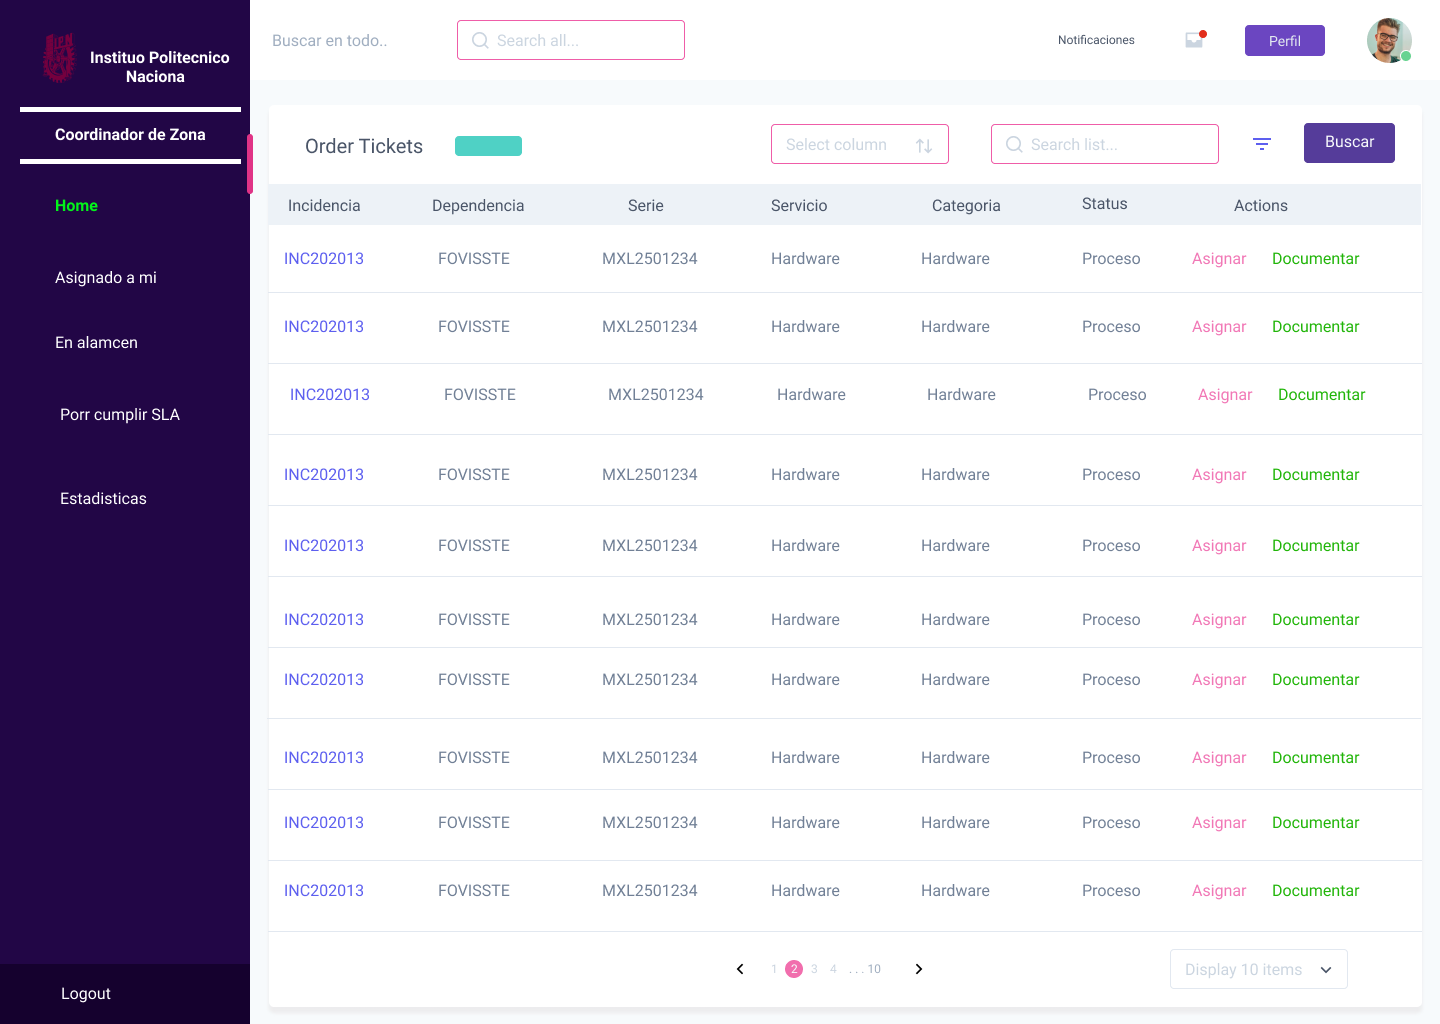
\includegraphics[width=1.1\textwidth]{Capitulo4/Img/GestionInc/Home}
	\caption{Interfaz- home de gestión de incidentes}
	\label{fig:IFDGDIH}
\end{figure}
Cuando se selecciona la acción es \textbf{\textit{	Documentación}}, se despliega una venta donde se encuentra los datos mas relevantes del ticket así como el seguimiento dado por los distintos usuarios que an contribuido a la solución tal como se muestra en la figura \ref{fig:IFDDTOPS}, así mismo esta  interfaz  dará dos posibles opciones a realizar, la primera se refiere a una nueva documentación y la segunda un cierre del ticket.

	\begin{figure}[H]
	\centering
	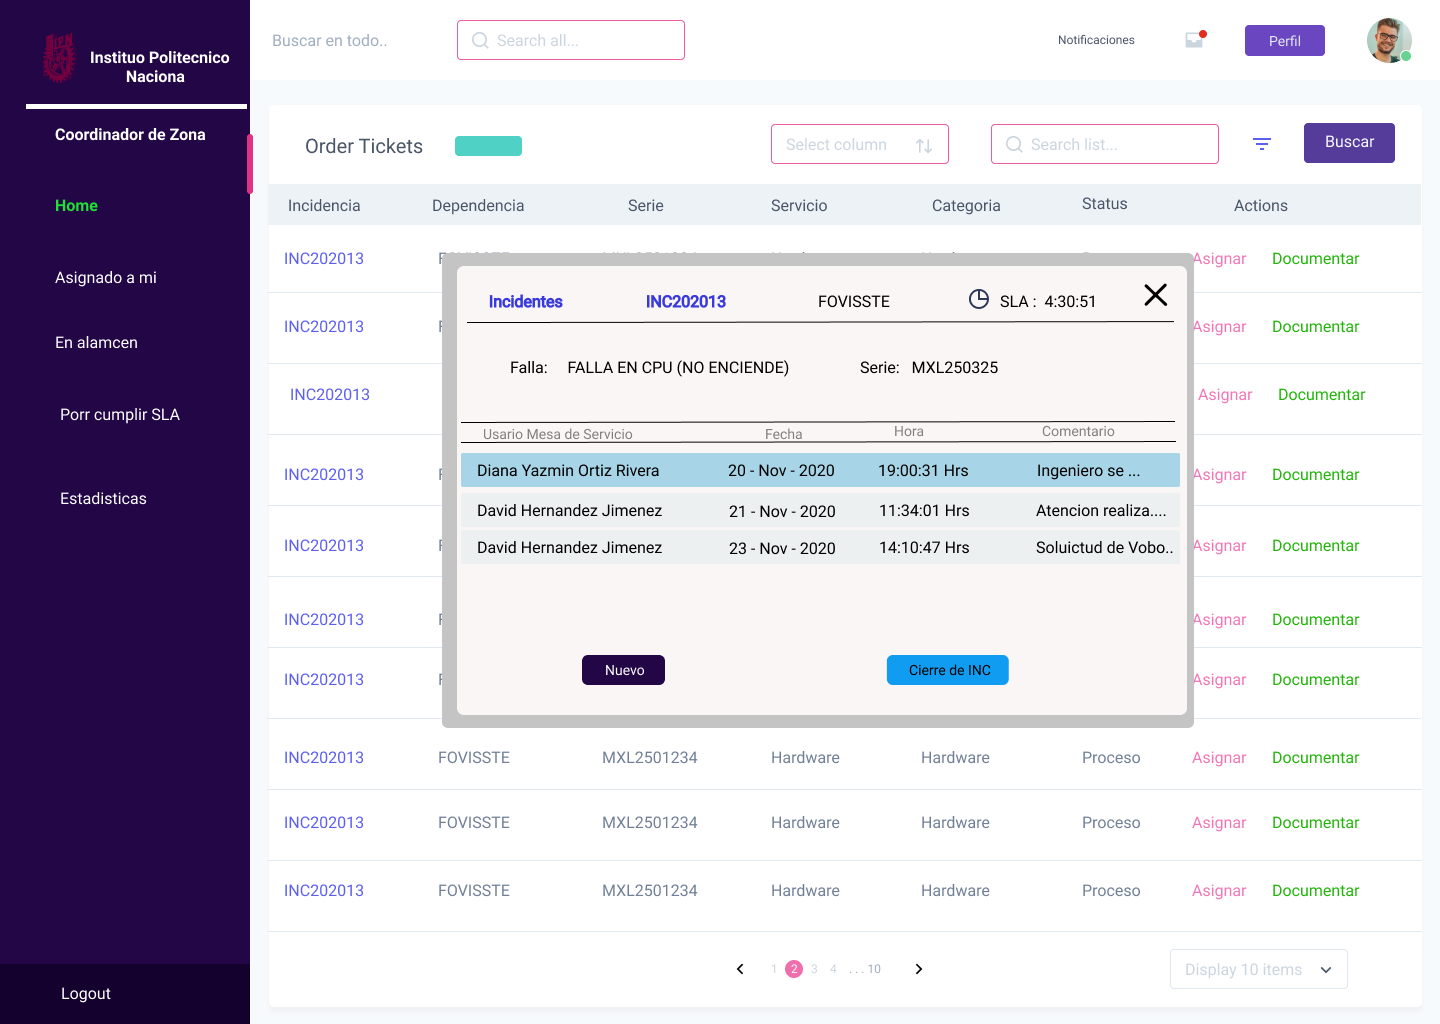
\includegraphics[width=1.1\textwidth]{Capitulo4/Img/GestionInc/Documentar-nuevo-seg}
	\caption{Interfaz- Opción de documentación o cierre de ticket }
	\label{fig:IFDDTOPS}
\end{figure}

Si la elección es \textbf{\textit{Nuevo }}  se actualizara la venta como se muestra en la figura \ref{fig:IFDSDTDOC} y se mostrara un cuadro de texto donde se realizara la documentación del ticket asi mismo se podrá adjuntar archivos, necesarios que contribuyan ala optima atención del ticket.

Cabe resaltar que dicha interfaz sera utilizada por los siguientes usuarios. 
\begin{itemize}
	\item Agente de mesa de servicio Nivel 1 
	\item Coordinador de zona Nivel 2
	\item Técnico especialista Nivel 2 
\end{itemize}

	\begin{figure}[H]
	\centering
	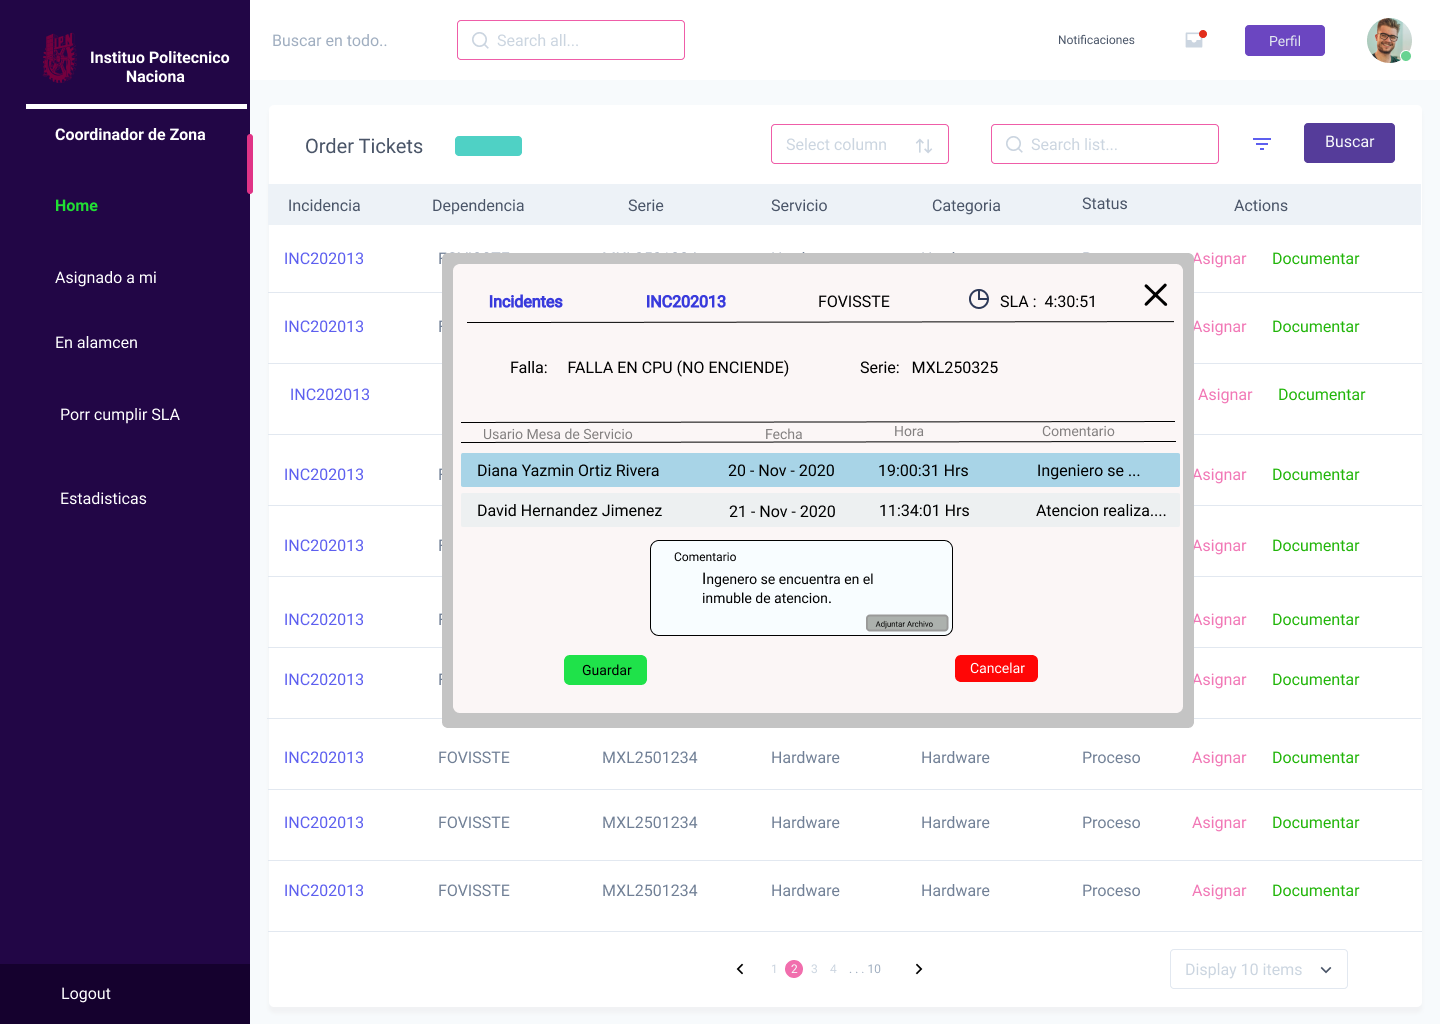
\includegraphics[width=1.1\textwidth]{Capitulo4/Img/GestionInc/Documentar-seg}
	\caption{Interfaz- Documentación de seguimiento Ticket}
	\label{fig:IFDSDTDOC}
\end{figure}

Si la acción seleccionada en la interfaz \ref{fig:IFDDTOPS} es \textbf{\textit{Cierre de INC}}, se actualizara la venta y se mostrara la  interfaz \ref{fig:IFDCDT}, donde se documentara el ticket y se adjuntara el correo de VoBo proporcionado por el usuario solicitante del servicio.

	\begin{figure}[H]
	\centering
	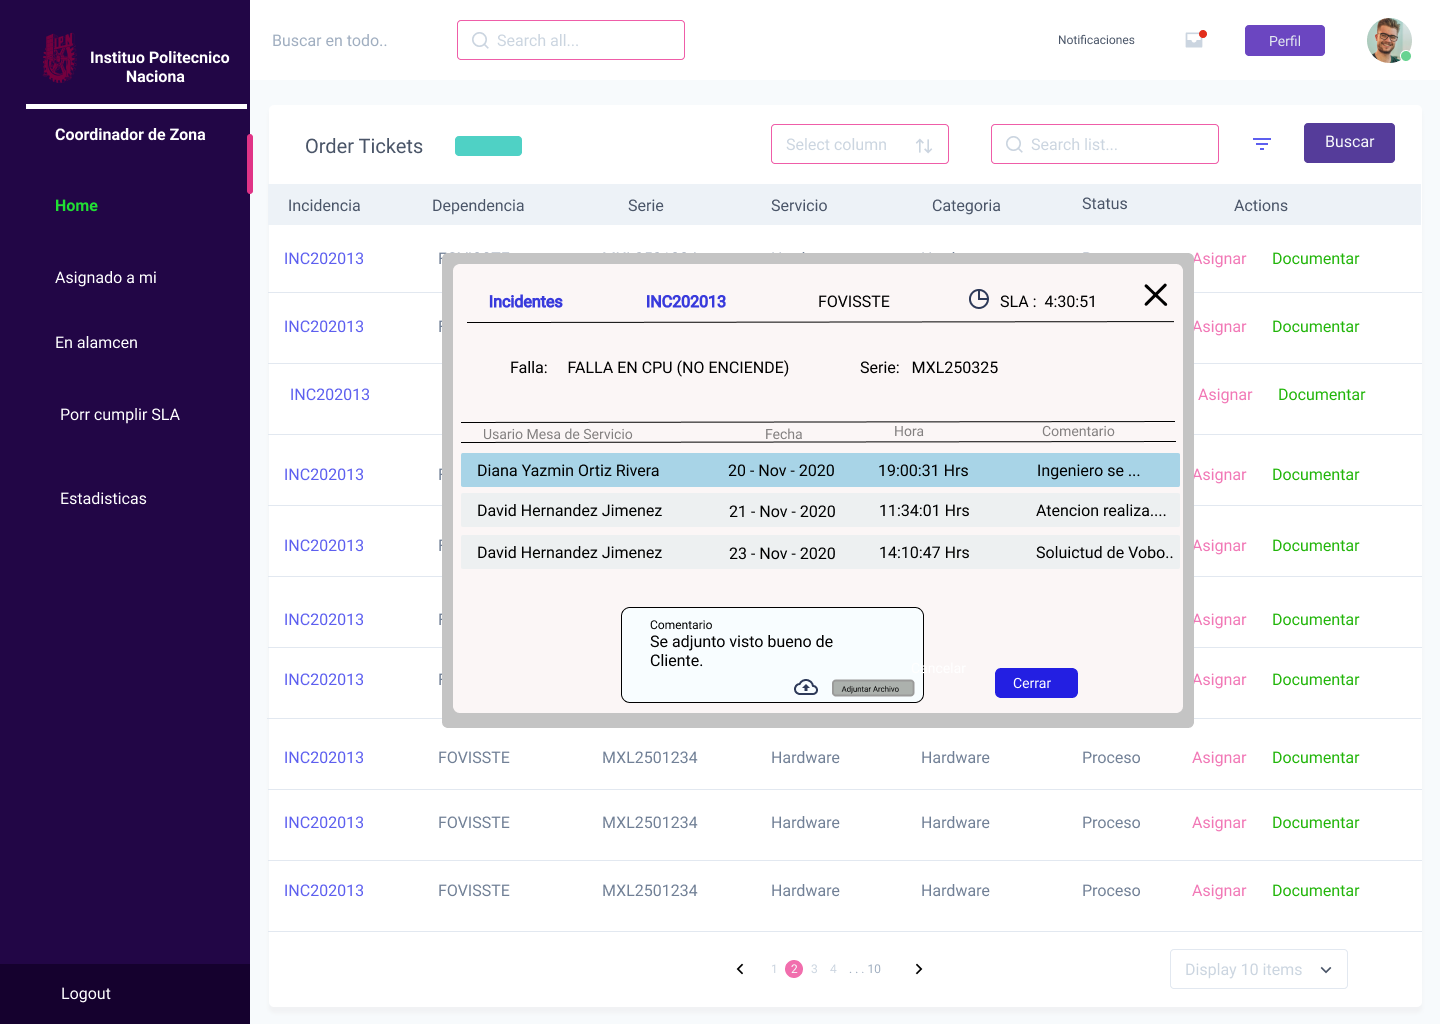
\includegraphics[width=1.1\textwidth]{Capitulo4/Img/GestionInc/cierre}
	\caption{Interfaz- Documentación de Cierre de Ticket}
	\label{fig:IFDCDT}
\end{figure}


Como se menciona anteriormente la interfaz de  \ref{fig:IFDGDIH}, cuenta con dos posibles acciones la primera documentaciones y la segunda asignacion, así mismo en la acción de asignacion, desplegara la asignacion de\textbf{\textit{ Sol. almacén}} la cual tiene como objetivo comenzar la solicitud de una refacción o varias piezas necesarias las cuales sean requeridas para atención del ticket, así como se puede ver en la interfaz \ref{fig:INDASAMC}  

	\begin{figure}[H]
	\centering
	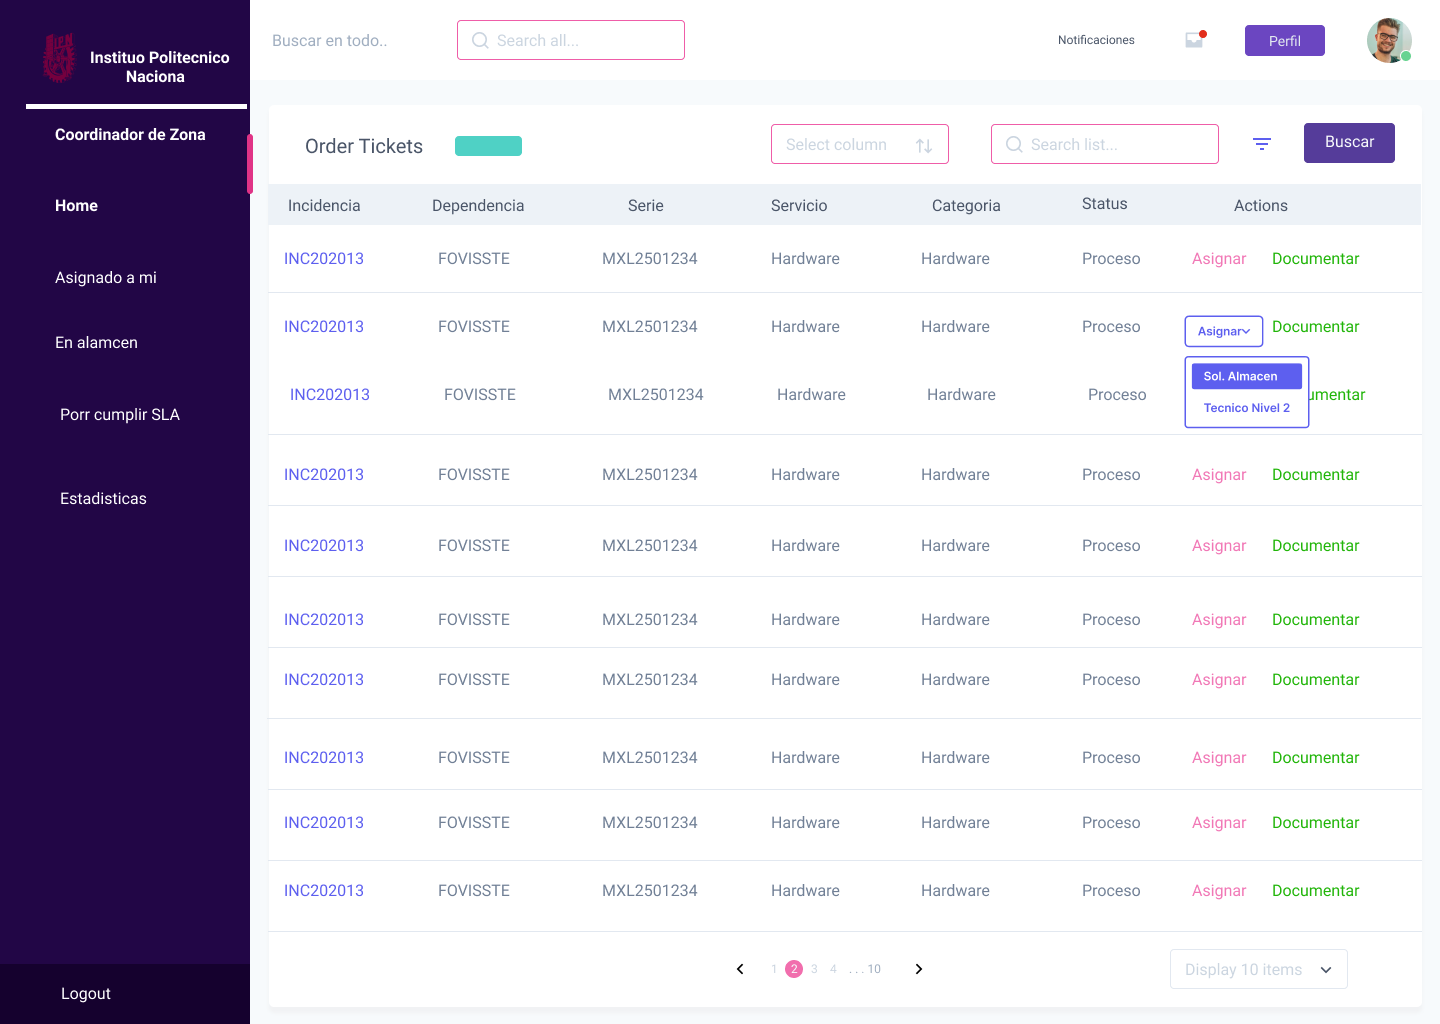
\includegraphics[width=1.1\textwidth]{Capitulo4/Img/GestionInc/Asi-Almacen}
	\caption{Interfaz- Asignacion a de solicitud a almacén}
	\label{fig:INDASAMC}
\end{figure}
Una vez iniciada la asignacion de una solicitud de almacenes, se desplegara la interfaz \ref{fig:RQSALINF} la cual mostrara información general del ticket así  como solicitara la Marca, Modelo, Tipo de equipo del cual se este solicitando de igual manera se mostrara un cuadro de texto, en el cual se podrá documentar algún requerimiento extra o alguna anotación.

Cabe resaltar que dicha interfaz sera utilizada por los siguientes usuarios. 



\begin{itemize}
	\item Coordinador de zona Nivel 2
	\item Técnico especialista Nivel 2 
\end{itemize}
	\begin{figure}[H]
	\centering
	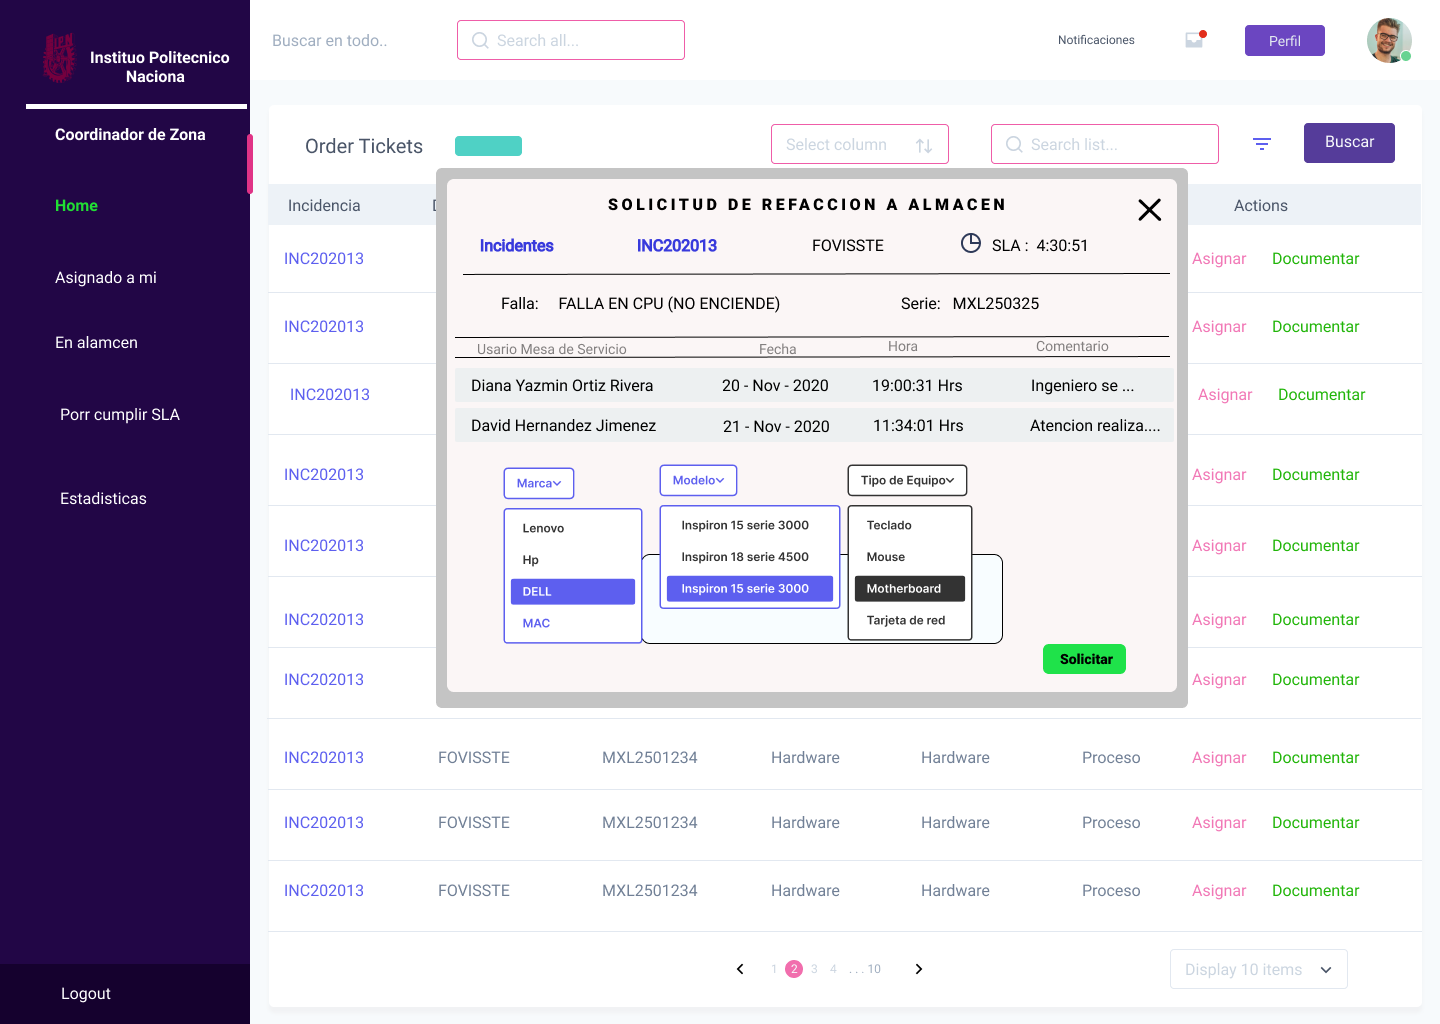
\includegraphics[width=1.1\textwidth]{Capitulo4/Img/GestionInc/Asi-almacen-sol}
	\caption{Interfaz- Requisición de solicitud a almacén}
	\label{fig:RQSALINF}
\end{figure}







\newpage
\subsection{Modulo de Gestión de Activos}
El modulo de gestión de activos tiene como objetivo dar el seguimiento a las refacciones o equipo ubicadas en el almacén con el fin de coordinar el almacén, así como generar los envíos necesarios de estas mismas refacciones a las distintas localidades donde se necesite dicha refacción.
\subsubsection{Requerimientos del módulo Gestión de Activos}
Para el correcto desarrollo del modulo de gestión de activos, se denotan los  requemamientos fundamentales para el funcionamiento de este mismo, siendo así descritos en la tabla \ref{tab:MDGDA}.

\begin{table}[H]
	\centering
	\caption{Requerimientos del modulo de gestión de activos}
	\begin{tabular}{|p{9.145em}|p{24.285em}|}
		\toprule
		\rowcolor[rgb]{ .125,  .216,  .392} \textcolor[rgb]{ 1,  1,  1}{\textbf{Requerimiento}} & \textcolor[rgb]{ 1,  1,  1}{\textbf{Descripción}} \\
		\midrule
		R11 & Registrar nuevo activo  \\
		\midrule
		R12 & Bajas de activos  \\
		\midrule
		R13 & Gestion de envios de activos  \\
		\bottomrule
	\end{tabular}%
	\label{tab:MDGDA}%
\end{table}%

\subsubsection{Descripción de caso de uso de Gestión de Activos}


\begin{multicols}{2}
	\textbf{Caso de uso: Gestión de Activos.}
	
	\begin{itemize}
		\item[$*$]  Actor principal
		\begin{itemize}
			\item Coordinador de almacén 
		\end{itemize}
		\item[$*$]  Objetivo en contexto
		\begin{itemize}
			\item Dar seguimiento a peticiones sobre refacciones.
			\item Documentar los envíos de refacciones.
			
		\end{itemize}
		\item[$*$]  Precondiciones
		\begin{itemize}
			\item Solo se atenderán la solicitud de envio de refacciones cuando el solicitante sea el Tecnico especialista.
			\item El coordinador de almacenes requiere estar autentificado en el sistema.
			
		\end{itemize}	
		\item[$*$]  Disparador
		\begin{itemize}
			\item Tecnico especialista Nivel 2 o Coordinador de zona, realizan un requerimiento de refacción del algún tipo al almacén.
		\end{itemize}
		\item[$*$]  Escenario
		\begin{itemize}
			\item Coordinador de zona o técnico especialista, solita una refacción a almacenes
			\item Coordinador de almacén recibe la  solicitud y verifica si hay en existencias.
			\item Coordinador genera una guía de envio para la refacción, dicha acción es documnetada en la herramienta. 
			\item Coordinador de almacen notifica a mesa de servicio que la pieza se encuentra en el destino. 
			\item Almecen genera una guía de retorno para la pieza dañada 
			
		\end{itemize}
		\item[$*$]  Excepciones
		\begin{itemize}
			\item Coordinador de almacen no puedo enviar mas reacciones de las que especificadas por mesa de servicio.		
		\end{itemize}
		\item[$*$]  Prioridad 
	\begin{itemize}
		\item Prioridad media 
	\end{itemize}
	\item[$*$]  Frecuencia de Uso
	\begin{itemize}
		\item Frecuencia media
	\end{itemize}
	\item[$*$]   Canal al actor.
	\begin{itemize}
		\item 	A través de un navegador con base en PC o LAPTOP y conexión a internet.
	\end{itemize}
	\item[$*$]  Actores secundarios
	\begin{itemize}
		\item Técnico especialista nivel 2
		\item Usuario, saltante del servicio
		
	\end{itemize}
\end{itemize}

\end{multicols}


\subsubsection{Actividades del proceso de Gestión de Activos}
La descripcion del proceso de gestión de activos, incluye  el subproceso de solicitud de piezas-refacción para la satisfactoria atención de la gestión de incidentes, dicho subproceso queda descrito en la tabla \ref{tab:TDPGDA}
  % Table generated by Excel2LaTeX from sheet 'Hoja10'
\begin{table}[H]
	\centering
	\caption{Actividades del proceso de Gestión de Activos}
\scalebox{0.40}{	\begin{tabular}{|c|c|c|c|}
		\toprule
		\rowcolor[rgb]{ .184,  .329,  .588} \multicolumn{4}{|p{59.285em}|}{\textcolor[rgb]{ 1,  1,  1}{Gestion de Activos - Almacen - Atencion de mesa de servicio }} \\
		\midrule
		\rowcolor[rgb]{ .184,  .329,  .588} \multicolumn{1}{|p{5.355em}|}{\textcolor[rgb]{ 1,  1,  1}{ID}} & \multicolumn{1}{p{9.5em}|}{\textcolor[rgb]{ 1,  1,  1}{Actividad}} & \multicolumn{1}{p{29.785em}|}{\textcolor[rgb]{ 1,  1,  1}{Descripción}} & \multicolumn{1}{p{14.645em}|}{\textcolor[rgb]{ 1,  1,  1}{Responsable}} \\
		\midrule
		1 & \multicolumn{1}{p{9.5em}|}{Solicitud de refaccion } & \multicolumn{1}{p{29.785em}|}{Coordinador de zona o Tecnico especialista, solicita una refaccion.} & \multicolumn{1}{p{14.645em}|}{Coordinador de zona \newline{}Tecnico especialista } \\
		\midrule
		2 & \multicolumn{1}{p{9.5em}|}{Notificacion a alamacen } & \multicolumn{1}{p{29.785em}|}{Coordinador de almacen visualiza en su home una nueva asigancion de requuemientos } & \multicolumn{1}{p{14.645em}|}{Coordinador de almacen } \\
		\midrule
		3 & \multicolumn{1}{p{9.5em}|}{Documentacion de despache } & \multicolumn{1}{p{29.785em}|}{Coordinador de almacen realiza la documentacion de la atencion.\newline{}\newline{}El ticket se documentara con la siguiente informacion:\newline{}\newline{}* Marca \newline{}* Modelo \newline{}* No. Serie \newline{}* Tipo de equipo \newline{}* Guia de envio - o ruta de envio\newline{}\newline{}Nota\newline{}-Si se cuenta con el recurso necesario para el requerimiento  pasar la actividad 4\newline{}- No se cuenta con el refaccion pasar a la actividad 4} & \multicolumn{1}{p{14.645em}|}{Coordinador de almacen } \\
		\midrule
		4 & \multicolumn{1}{p{9.5em}|}{Ticket en espere} & \multicolumn{1}{p{29.785em}|}{El ticket se documentara haciendo informe de la espera de refaccion para su despache.} & \multicolumn{1}{p{14.645em}|}{Coordinador de almacen } \\
		\midrule
		5 & \multicolumn{1}{p{9.5em}|}{Docuemntacion de atencion } & \multicolumn{1}{p{29.785em}|}{Coordinador de almacen documenta el cierre de la atencion, con una  guia de retorno para la pieza dañada. } & \multicolumn{1}{p{14.645em}|}{Coordinador de almacen } \\
		\midrule
		&   &   &  \\
		\bottomrule
	\end{tabular}%
	\label{tab:TDPGDA}}%
\end{table}%


En la tabla \ref{tab:TDGDAABA} se describen los procesos subsecuentes que tendrá el modulo de Gestión de activos, los cuales se describen como altas, actualización y bajas de activos. 



  % Table generated by Excel2LaTeX from sheet 'Hoja10'
\begin{table}[H]
	\centering
	\caption{Gestion de activos- altas. actualización y bajas}
\scalebox{0.40}{\begin{tabular}{|c|c|l|c|}
		\toprule
		\rowcolor[rgb]{ .184,  .329,  .588} \multicolumn{4}{|p{59.285em}|}{\textcolor[rgb]{ 1,  1,  1}{Gestion de Activos - Almacen - Bajas y altas de Activos }} \\
		\midrule
		\rowcolor[rgb]{ .184,  .329,  .588} \multicolumn{1}{|p{5.355em}|}{\textcolor[rgb]{ 1,  1,  1}{ID}} & \multicolumn{1}{p{9.5em}|}{\textcolor[rgb]{ 1,  1,  1}{Actividad}} & \multicolumn{1}{p{29.785em}|}{\textcolor[rgb]{ 1,  1,  1}{Descripción}} & \multicolumn{1}{p{14.645em}|}{\textcolor[rgb]{ 1,  1,  1}{Responsable}} \\
		\midrule
		1 & \multicolumn{1}{p{9.5em}|}{Agragar un nuevo activo } & \multicolumn{1}{p{29.785em}|}{El coordinador de almacen, agrega un nuevo activo al inventario de almacen, el cual sera capturado con la siguiente informacion: \newline{}* Marca \newline{}* Modelo  \newline{}* Tipo de equipo \newline{}* Cantidad en inventario \newline{}} & \multicolumn{1}{p{14.645em}|}{Coordinador de almacen } \\
		\midrule
		2 & \multicolumn{1}{p{9.5em}|}{Actulizacion de Activo } & \multicolumn{1}{p{29.785em}|}{El coordinador de almacen, ACTULIZARA un  activo del  inventario de almacen, el cual unicamente podra ser actulizado en su cantidad\newline{}* Marca \newline{}* Modelo \newline{}* Tipo de equipo \newline{}* Cantidad en inventario \newline{}} & \multicolumn{1}{p{14.645em}|}{Coordinador de almacen } \\
		\midrule
		3 & \multicolumn{1}{p{9.5em}|}{Eliminacion de Activo } & \multicolumn{1}{p{29.785em}|}{El coordinador de almacen,ELIMINARA un activo del inventario de almacen, cuando este sea descontinuado, asi mismo de describira el motivo de la eliminacion de dicho activo. } & \multicolumn{1}{p{14.645em}|}{Coordinador de almacen } \\
		\midrule
		&   &   &  \\
		\bottomrule
	\end{tabular}%
	\label{tab:TDGDAABA}}%
\end{table}%

\subsubsection{Diagrama de secuencia - Gestión de Activos}

La descripcion de la gestión de activos en esta sección solo implicara la relación de atención de un servicio de despacho de suministros para porta del almacén hacia la atención de los incidentes generados por operación como se muestra en el diagrama de secuencia \ref{fig:GDADDF} .


\begin{figure}[H]
	\centering
	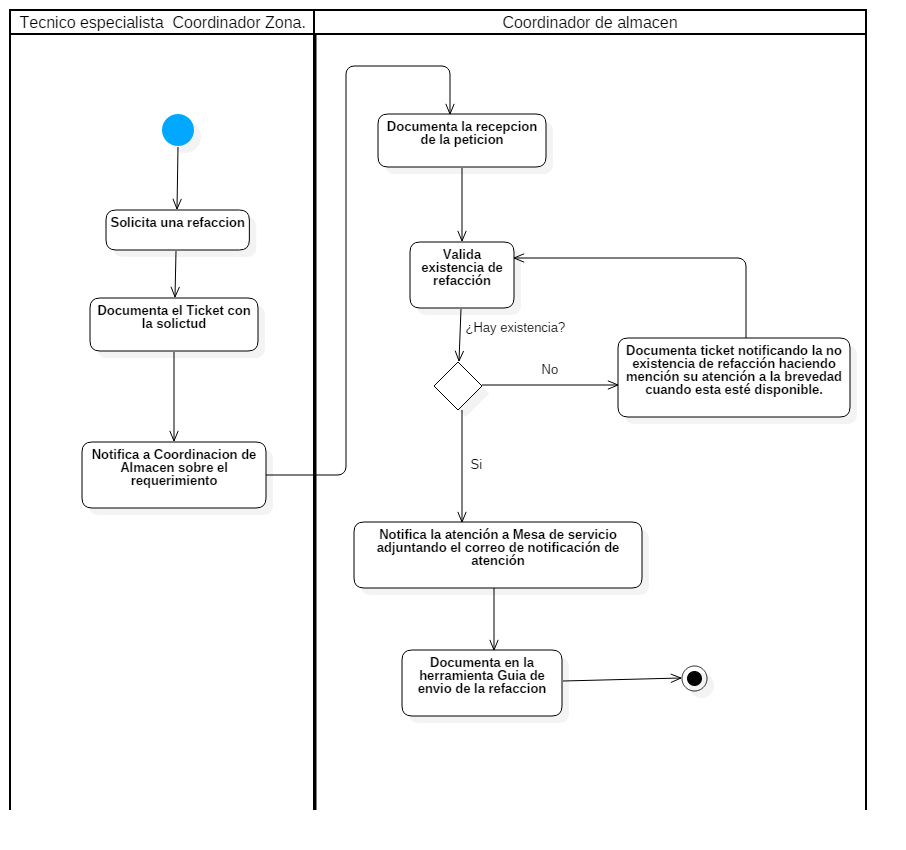
\includegraphics[width=0.9\textwidth]{Capitulo4/Img/GestionAc/GestionActivos}
	\caption{Diagrama de secuencia - "Gestiona de Activos"}
	\label{fig:GDADDF}
	\end{figure}
	

\subsubsection{Interfaz de Grafica - Gestión de Activos}
La gestión de activos comienza su interacción con el sistema cuando un coordinador de zona o un técnico especialista, hacen un requerimiento de una refacciona o pieza para la atención del ticket, por lo cual almacenes contara con una interfaz home donde se mostrara todas las acciones que se podrán hacer en el sistema, como se muestra en la interfaz  \ref{fig:HOGDAAL}, por consiguiente la interfaz tendrá  dos acciones relevantes, la primera Despachar y la segunda Documentación.

	\begin{figure}[H]
	\centering
	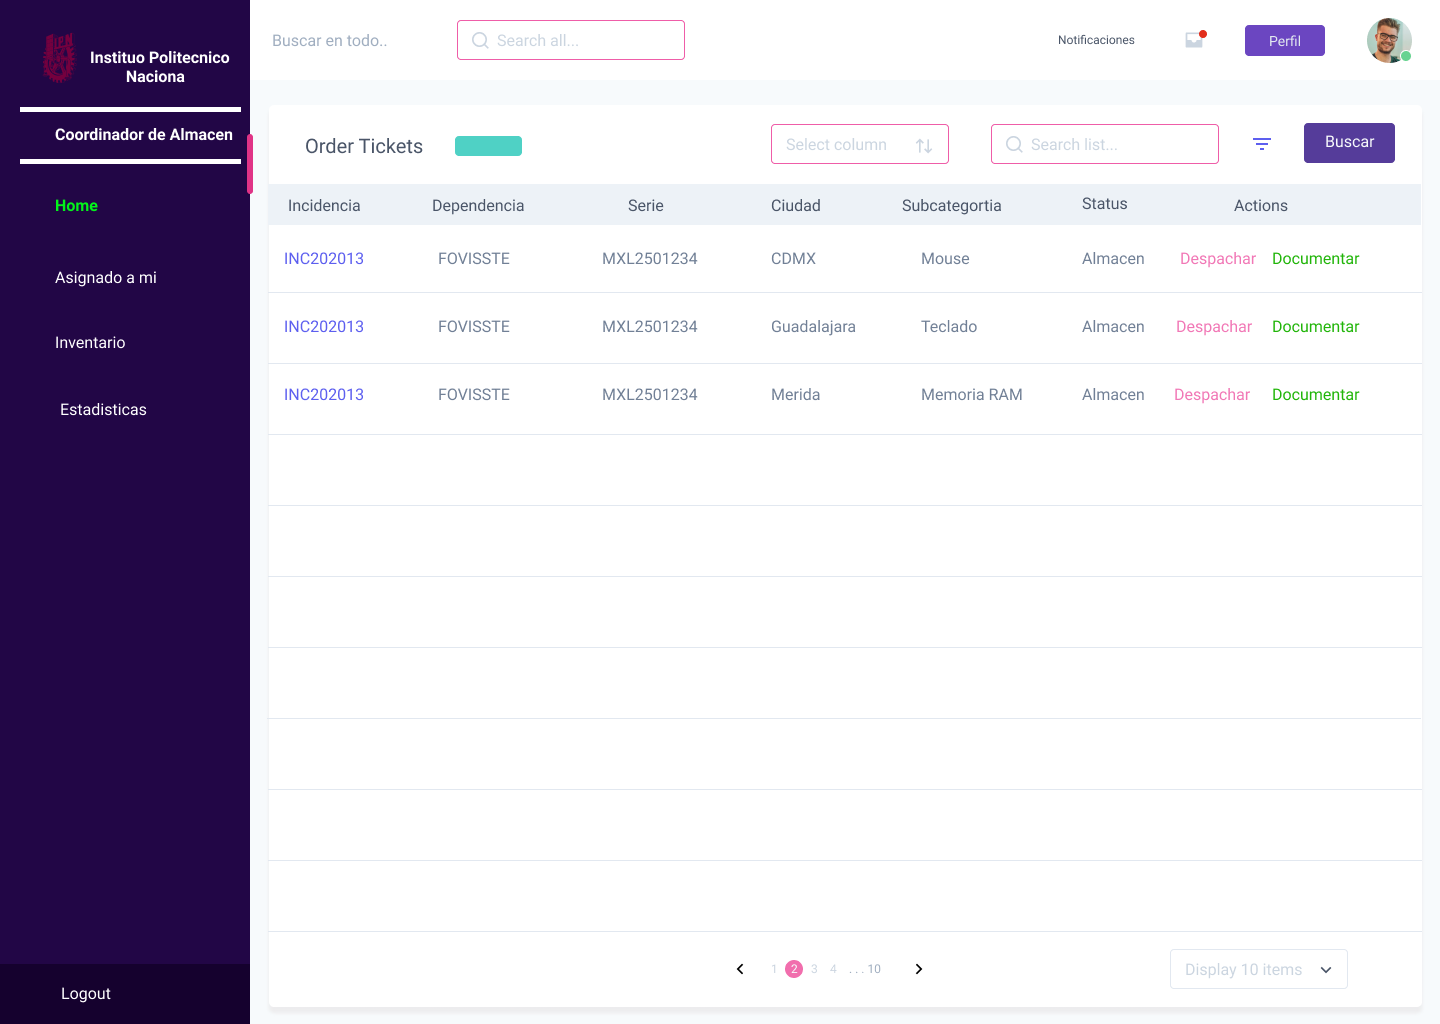
\includegraphics[width=1.1\textwidth]{Capitulo4/Img/GestionAc/Home}
	\caption{Interfaz- Home de gestión de activos}
	\label{fig:HOGDAAL}
\end{figure}



Cuando se selecciona la acción es \textbf{\textit{Documentación}}, se despliega una venta donde se encuentra los datos mas relevantes del ticket así como el seguimiento dado por los distintos usuarios que an contribuido a la solución tal como se muestra en la figura \ref{fig:DODACTICVOS}.

\begin{figure}[H]
	\centering
	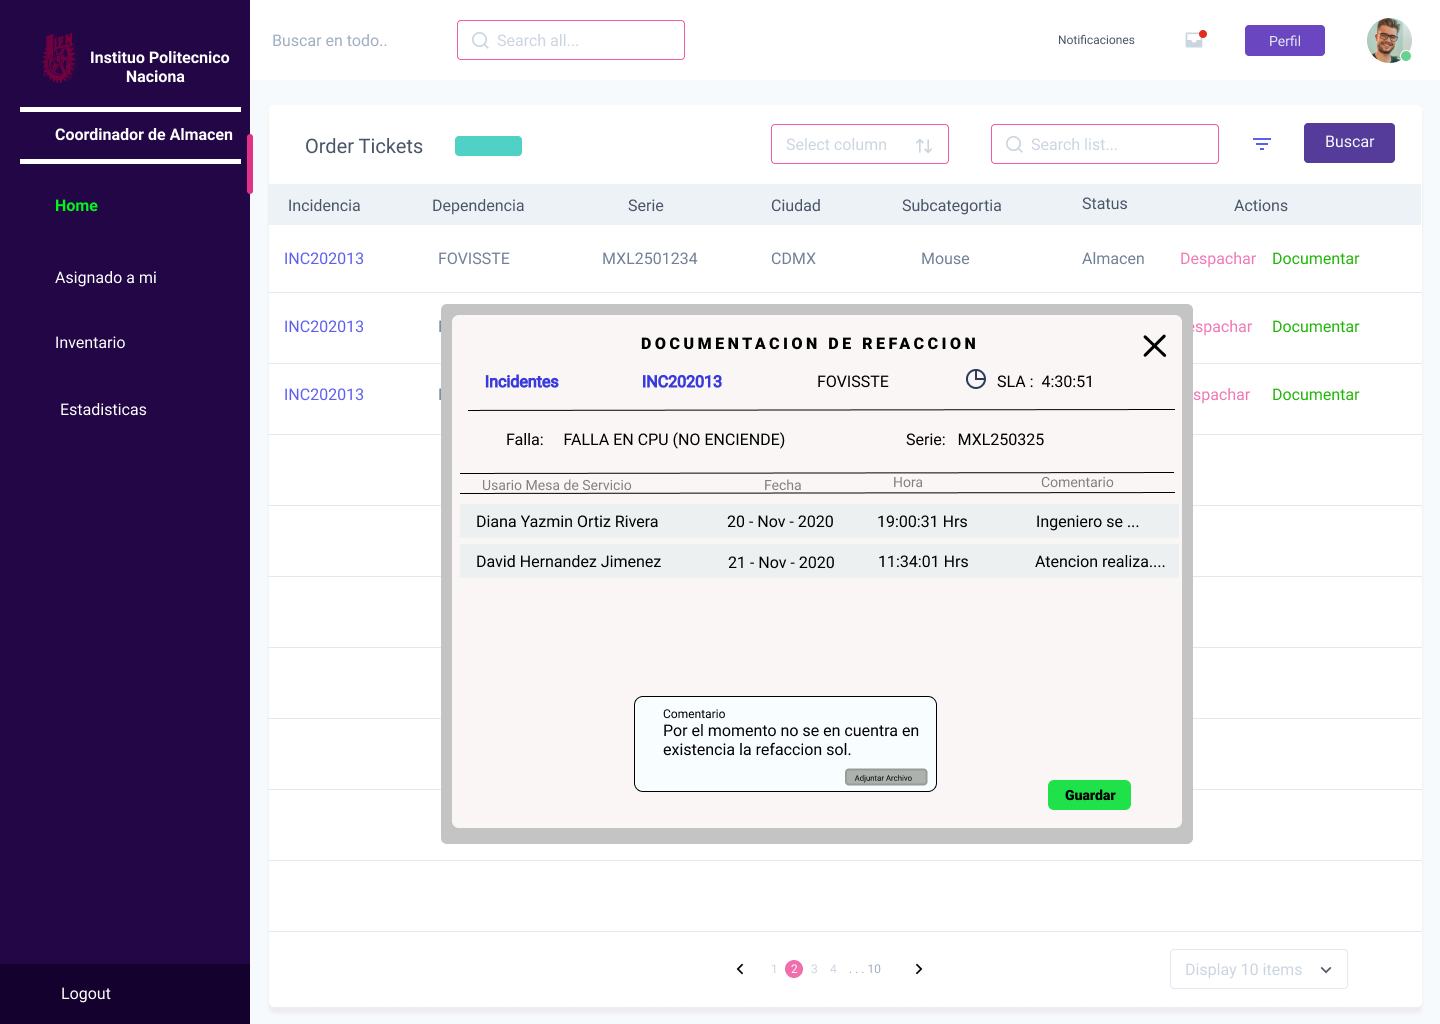
\includegraphics[width=1.1\textwidth]{Capitulo4/Img/GestionAc/Almacen-Doc}
	\caption{Interfaz- Documentación de solicitud de activo }
	\label{fig:DODACTICVOS}
\end{figure}

Si la acción  seleccionada es  \textbf{\textit{\underline{Despacho}}} se desplegara la siguiente interfaz \ref{fig:DESALM} donde se mostrara los datos generales así como un formulario donde se llenara con los datos de la refacción a despachar, así mismo se registrara el numero de guía de envió, si es el caso, cuando se haya completado el formulario, se dará clcik en guardar y el ticket sera notificado a coordinador de zona o técnico especialista sobre la atención de almacén.

\begin{figure}[H]
	\centering
	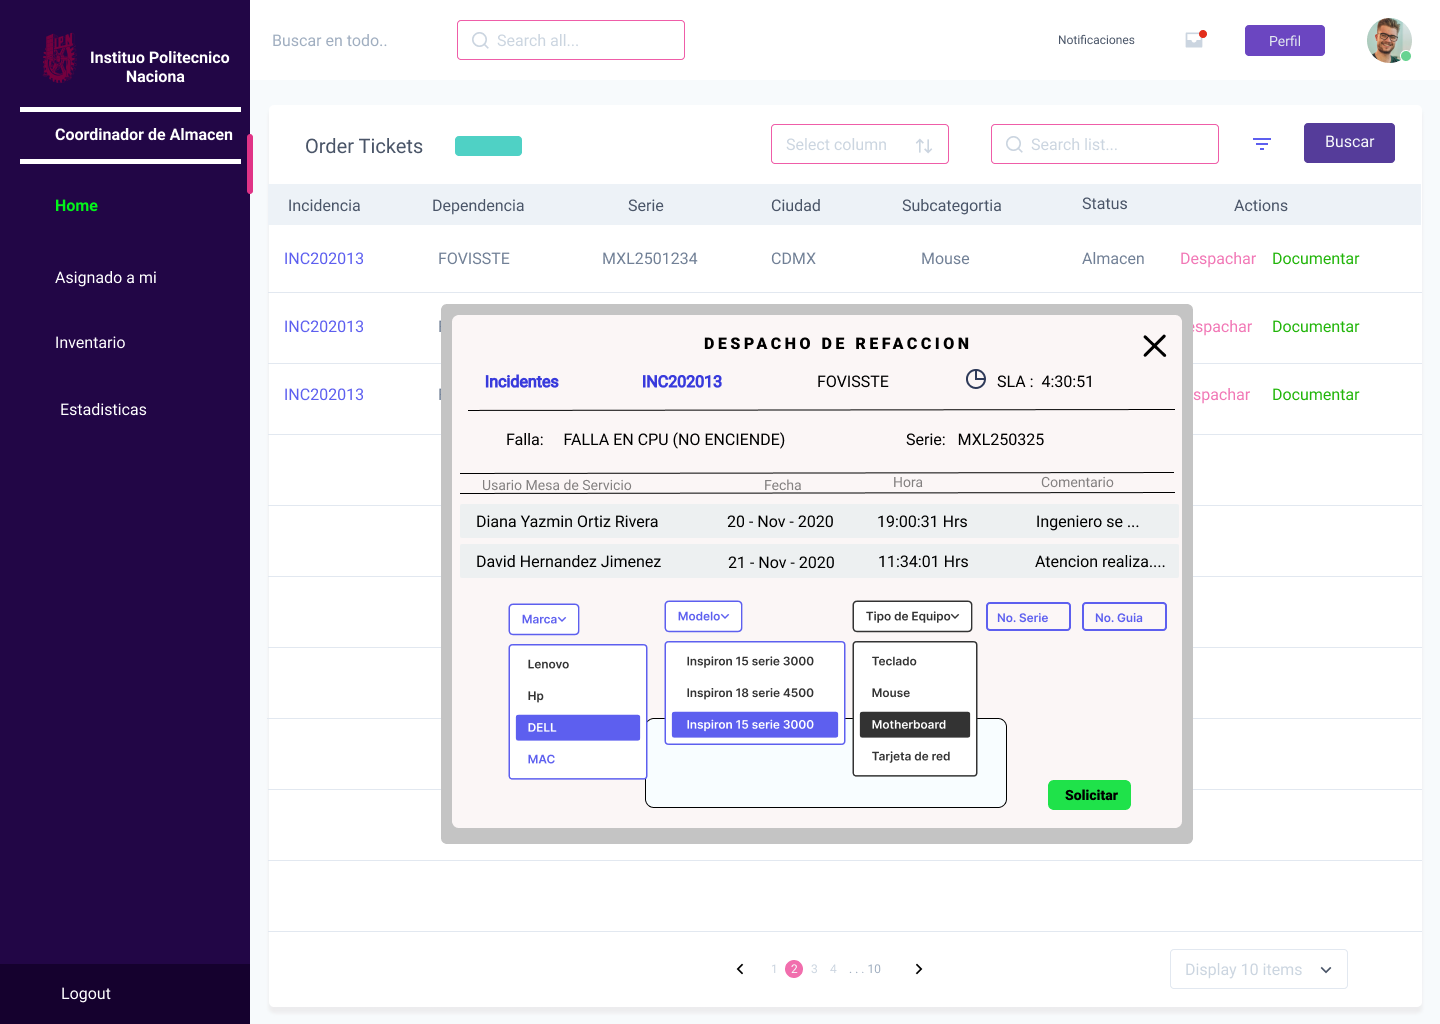
\includegraphics[width=1.1\textwidth]{Capitulo4/Img/GestionAc/Almacen-despachar}
	\caption{Interfaz- Despacho de refacción  }
	\label{fig:DESALM}
\end{figure}






\subsubsection{Diagrama de clases - Gestión de Activos}



\newpage
\subsection{Modulo de Gestión de informes}
El modulo de Reportes, tiene como objetivo dar a conocer de una forma grafica así como cuantitativa las métricas del proceso de mesa de servicio, 
donde se describirá la eficiencia del proceso de atención.
\subsubsection{Requerimientos del módulo de Gestión de informes}

Los requerimientos del modulo se describirán por usuario, ya que cada usuario tendrá una lista de reportes relacionados con su rol en la mesa de servicio, estos reportes se muestran en la tabla \ref{tab:RFRP}

   % Table generated by Excel2LaTeX from sheet 'Hoja11'
 \begin{table}[H]
 	\centering
 	\caption{Requerimientos del modulo de Gestión de informes}
 \scalebox{0.55}{	\begin{tabular}{|c|p{9.145em}|p{28.145em}|}
 		\toprule
 		\rowcolor[rgb]{ .125,  .216,  .392} \multicolumn{1}{|p{9.355em}|}{\textcolor[rgb]{ 1,  1,  1}{\textbf{Usuario }}} & \textcolor[rgb]{ 1,  1,  1}{\textbf{Requerimiento}} & \textcolor[rgb]{ 1,  1,  1}{\textbf{Descripción}} \\
 		\midrule
 		\multicolumn{1}{|c|}{\multirow{5}[10]{*}{Agente de mesa de servicio Nivel 1}} & R14 & Tickets Aperturados por mes  \\
 		\cmidrule{2-3}        & R15 & Incidencias atendidas por mes  \\
 		\cmidrule{2-3}        & R16  & Estatus de incidentes  \\
 		\cmidrule{2-3}        & R17 & Incidentes por dependencia  \\
 		\cmidrule{2-3}        & R18 & Incidentes por estado  \\
 		\midrule
 		\multicolumn{1}{|c|}{\multirow{4}[8]{*}{Coordinadoer de Zona }} & R19 & Incidencias atendidas por mes  \\
 		\cmidrule{2-3}        & R20 & Estatus de incidentes  \\
 		\cmidrule{2-3}        & R21 & Incidentes por dependencia  \\
 		\cmidrule{2-3}        & R22 & Incidentes por estado  \\
 		\midrule
 		\multirow{3}[6]{*}{Tecnico especialista } & R23 & Incidencias atendidas por mes  \\
 		\cmidrule{2-3}        & R24 & Estatus de incidentes  \\
 		\cmidrule{2-3}        & R25 & Incidentes por dependencia  \\
 		\midrule
 		\multicolumn{1}{|c|}{\multirow{5}[10]{*}{Gerente de Mesa de servicio }} & R26 & \multicolumn{1}{l|}{Tickets aperturados por mes } \\
 		\cmidrule{2-3}        & R27 & Tickets cerrados por mes, año y por depencia  \\
 		\cmidrule{2-3}        & R28 & Tickets cerrados por ciudad en tiempos de 1 mes y por año  \\
 		\cmidrule{2-3}        & R29 & tickets en Proceso, por dependecia  \\
 		\cmidrule{2-3}        & R30 & Servicios mas recurrentes  \\
 		\bottomrule
 	\end{tabular}%
 	\label{tab:RFRP}}%
 \end{table}%



\subsubsection{Descripción de caso de uso de Gestión de informes}

\begin{multicols}{2}
	\textbf{Caso de uso: Gestión de informes.}
	
	\begin{itemize}
		\item[$*$]  Actor principal
		\begin{itemize}
			\item Gerente de mesa de servicio 
		\end{itemize}
		\item[$*$]  Objetivo en contexto
		\begin{itemize}
			\item Dar información en forma gráfica.
			\item Proporcionar información cuantitativa.
		\end{itemize}
		\item[$*$]  Precondiciones
		\begin{itemize}
			\item El usuario, tiene que tener por lo menos 1 mes de trabajo previo.
			\item Los usuarios solicitantes de la información deben estar autentificados en el sistema.
			
		\end{itemize}	
		\item[$*$]  Disparador
		\begin{itemize}
			\item El usuario del sistema, requiere información de estadísticas.
		\end{itemize}
			\item[$*$]  Escenario
			\begin{itemize}
				\item El usuario del da click sobre el icono de dashboard
				\item Se muestra las  información que puede proporcionar el sistema. 
			\end{itemize}
			
			\item[$*$]  Prioridad 
		\begin{itemize}
			\item Prioridad baja 
		\end{itemize}
		\item[$*$]  Frecuencia de Uso
		\begin{itemize}
			\item Frecuencia baja
		\end{itemize}
		\item[$*$]   Canal al actor.
		\begin{itemize}
			\item 	A través de un navegador con base en PC o LAPTOP y conexión a internet.
		\end{itemize}
		\item[$*$]  Actores secundarios
		\begin{itemize}
			\item Técnico especialista nivel 2
			\item Coordinador de zona
			\item Agente de mesa de servicio.
		\end{itemize}
\end{itemize}

\end{multicols}


\subsubsection{Interfaz de Grafica - Gestión de informes}





El modulo de informes estará compuesto por aquellas requisiciones  de los usuarios miembros del sistema, estos reportes estarán relacionados directamente con las actividades desempeñados, por lo que se genera en istogramos como en graficas de pastel, haciendo que la información sea concisa y rápida de leer, como se muestra en la interfaz  \ref{fig:GDINFOE}.


\begin{figure}[h]
	\centering
	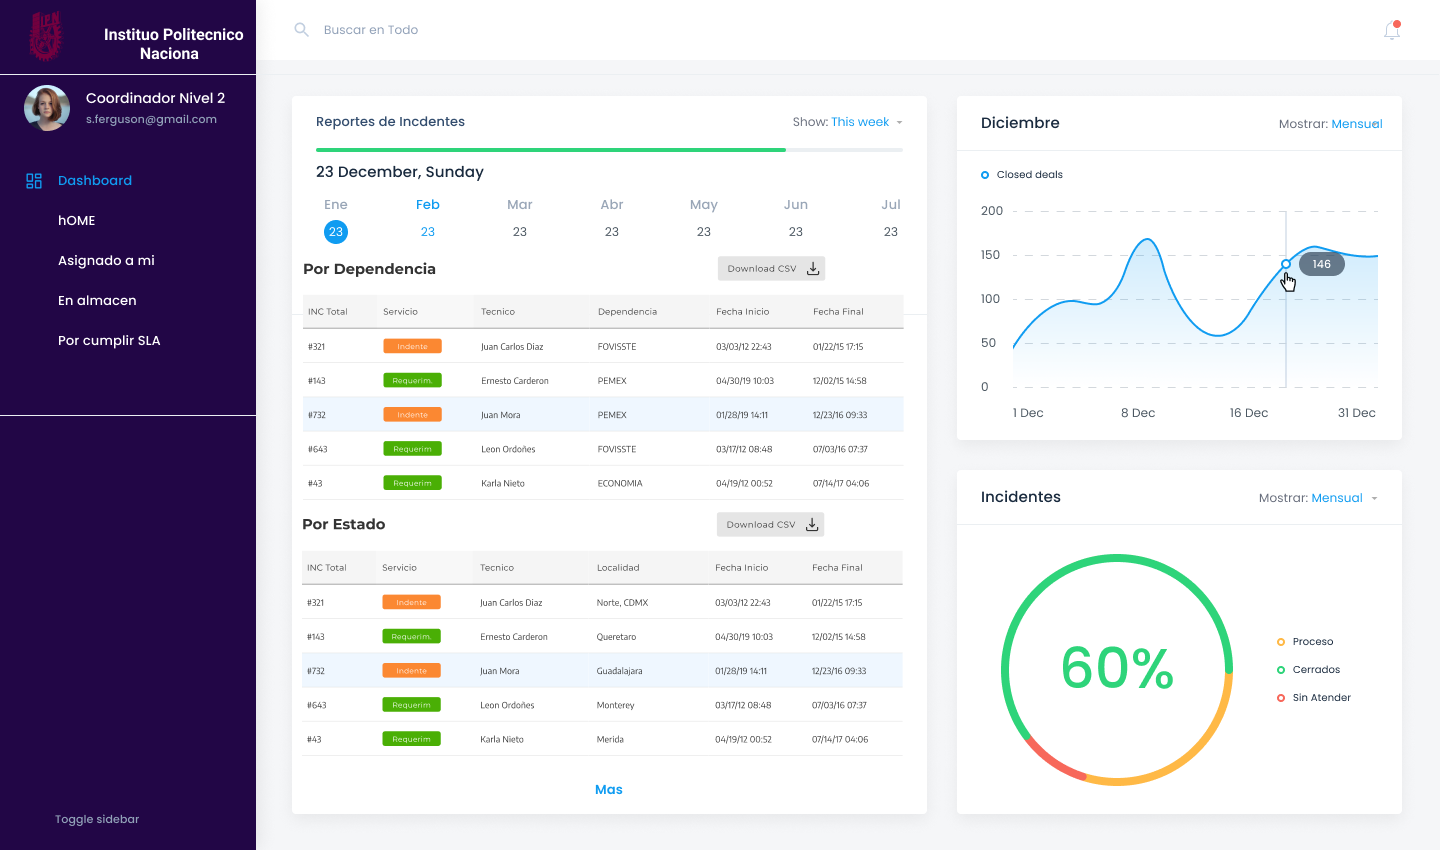
\includegraphics[width=1.1\textwidth]{Capitulo4/Img/GestionInf/informes}
	\caption{Interfaz - Gestión de informes}
	\label{fig:GDINFOE}
\end{figure}



\newpage

\subsection{Modulo de Gestión de usuarios del sistema}
Este módulo será el que implemente la interfaz de gestión de
usuarios por lo cual  realizara las acciones on-line, genere peticiones de usuario para las acciones
diferidas y permita la gestión de peticiones generadas y la consulta de información de los diferentes integrantes del sistemas.

El principal usuario del sistema es el usuario administrador con privilegios para la
administración y gestión de los usuarios del sistema. Una vez validado, este
usuario será quien tenga permiso para efectuar las diferentes funcionalidades que ofrece
el módulo gestión de usuarios. 
\subsubsection{Requerimientos del módulo de gestión de usuarios}
El modulo de gestión de usuarios, para el correcto desempeño de las actividades propuestas, se describen los requermientos necesarios para llegar a la eficiencia como se muestra en la tabla \ref{tab:RFDGDU}


  % Table generated by Excel2LaTeX from sheet 'Hoja12'
\begin{table}[H]
	\centering
	\caption{Requerimientos de modulo de gestión de usuarios }
 \scalebox{0.55}{	\begin{tabular}{|p{9.145em}|p{28.145em}|}
		\toprule
		\rowcolor[rgb]{ .125,  .216,  .392} \textcolor[rgb]{ 1,  1,  1}{\textbf{Requerimiento}} & \textcolor[rgb]{ 1,  1,  1}{\textbf{Descripción}} \\
		\midrule
		R31 & Consulta datos Usuarios  \\
		\midrule
		R32 & Bloqueo de Usuarios  \\
		\midrule
		R33 & Desbloqueo de Usuarios  \\
		\midrule
		R34 & Modificación de contraseñas  \\
		\midrule
		R35 & Asignacion de permisos  \\
		\midrule
		R36 & Consulta de permisos  \\
		\midrule
		R37 & Alta de usuario  \\
		\midrule
		R38 & Solicitud de asignacion perfil de usuario  \\
		\midrule
		R39 & Eliminación de usuarios \\
		\bottomrule
	\end{tabular}}%
	\label{tab:RFDGDU}%
\end{table}%

\subsubsection{Descripcion de casos de usos del modulo - Gestión de usuarios }
Se presenta el caso de uso del modulo de gestión de usuarios como se muestra en la figura \ref{fig:DDCDUGDUSER}

\begin{figure}[H]
	\centering
	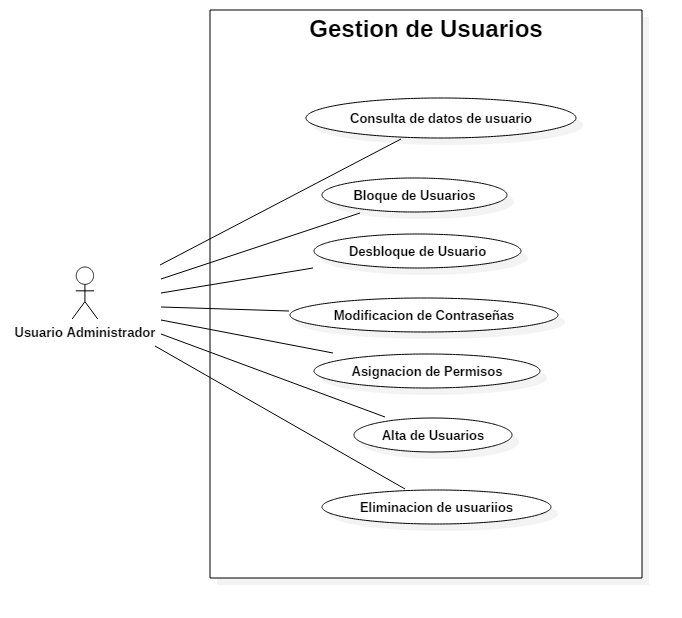
\includegraphics[width=0.75\textwidth]{Capitulo4/Img/GestionUser/Gestion_User}
	\caption{Interfaz - Caso de Uso Modulo de gestión de usuarios}
	\label{fig:DDCDUGDUSER}
\end{figure}

Este apartado facilita una descripción detallada de los diferentes casos de uso del modulo de gestión de usuarios.

\textbf{\textit{Descripcion del caso de Bloque de Usuarios.}}.

En la tabla \ref{tab:CDUSBLDU} se describe la ejecución del caso de bloquear usuarios.

  % Table generated by Excel2LaTeX from sheet 'Hoja13'
\begin{table}[H]
	\centering
	\caption{Caso de uso-bloqueo de usuarios}
 \scalebox{0.85}{	\begin{tabular}{|l|p{26.645em}|}
		\toprule
		\rowcolor[rgb]{ .125,  .216,  .392} \multicolumn{2}{|p{37.5em}|}{\textcolor[rgb]{ 1,  1,  1}{\textbf{BLOQUEO DE USUARIOS }}} \\
		\midrule
		\textbf{Caso de uso } & \multicolumn{1}{l|}{Bloquear usuario. } \\
		\midrule
		\textbf{Actores } & \multicolumn{1}{l|}{Usuario administrador.} \\
		\midrule
		\textbf{Objetivo } & \multicolumn{1}{l|}{Bloquear un usuario del sistema. } \\
		\midrule
		\textbf{Descripción } & Bloquea el usuario seleccionado para impedir su acceso al sistema.  \\
		\midrule
		\textbf{Precondiciones} & \multicolumn{1}{l|}{Usuario seleccionado no bloqueado. } \\
		\midrule
		\textbf{Postcondiciones} & \multicolumn{1}{l|}{Usuario bloqueado. } \\
		\midrule
		\textbf{Flujo normal } & 1. El usuario selecciona un usuario no bloqueado de la lista\newline{}de usuarios del departamento.\newline{}2. El usuario selecciona la opción bloquear usuario\newline{}3. El usuario confirma acción.\newline{}4. El sistema modifica a bloqueado el estado del usuario.\newline{}5. El sistema incluye una marca indicativa de usuario\newline{}bloqueado en la lista de usuarios del departamento.\newline{}6. El sistema habilita la opción desbloquear usuario.  \\
		\midrule
		\textbf{Flujo alternativo} & 1. En caso de (cancelar acción) el sistema finaliza la acción sin efectuar cambios. \newline{}2. En caso de (error de actualización de BD) el sistema muestra un mensaje indicativo. \\
		\bottomrule
	\end{tabular}%
	\label{tab:CDUSBLDU}}%
\end{table}%
\textbf{\textit{Descripcion del caso de Desbloqueo de Usuarios.}}.

En la tabla \ref{tab:DDCDDUSIOS} se describe la ejecución del caso de desbloquear usuarios.
  % Table generated by Excel2LaTeX from sheet 'Hoja14'
\begin{table}[H]
	\centering
	\caption{Caso de uso-desbloqueo de usuarios}
\scalebox{0.85}{	\begin{tabular}{|r|r|}
		\toprule
		\rowcolor[rgb]{ .125,  .216,  .392} \multicolumn{2}{|p{42.855em}|}{\textcolor[rgb]{ 1,  1,  1}{\textbf{DESBLOQUEAR USUARIO }}} \\
		\midrule
		\multicolumn{1}{|l|}{\textbf{Caso de uso }} & \multicolumn{1}{l|}{Desbloquear usuario. } \\
		\midrule
		\multicolumn{1}{|l|}{\textbf{Actores }} & \multicolumn{1}{l|}{Usuario administrador.} \\
		\midrule
		\multicolumn{1}{|l|}{\textbf{Objetivo }} & \multicolumn{1}{l|}{Desbloquear un usuario del sistema. } \\
		\midrule
		\multicolumn{1}{|l|}{\textbf{Descripción }} & \multicolumn{1}{l}{Desbloquea el usuario seleccionado para permitir su acceso al sistema.} \\
		\midrule
		\multicolumn{1}{|l|}{\textbf{Precondiciones}} & \multicolumn{1}{l|}{Usuario seleccionado bloqueado. } \\
		\midrule
		\multicolumn{1}{|l|}{\textbf{Postcondiciones}} & \multicolumn{1}{l|}{Usuario desbloqueado. } \\
		\midrule
		\multicolumn{1}{|l|}{\textbf{Flujo normal }} & \multicolumn{1}{p{32em}|}{1. El usuario selecciona un usuario bloqueado de la lista de\newline{}usuarios del departamento.\newline{}2. El usuario selecciona la opción desbloquear usuario.\newline{}3. El usuario confirma acción.\newline{}4. El sistema modifica a desbloqueado el estado del usuario.\newline{}5. El sistema elimina la marca de usuario bloqueado de la\newline{}lista de usuarios del departamento.\newline{}6. El sistema habilita la opción bloquear usuario. } \\
		\midrule
		\multicolumn{1}{|l|}{\textbf{Flujo alternativo}} & \multicolumn{1}{p{32em}|}{1. En caso de (cancelar acción) el sistema finaliza la\newline{}acción sin efectuar cambios.\newline{}2. En caso de (error de actualización de BD) el sistema\newline{}muestra un mensaje indicativo. } \\
		\midrule
		&  \\
		\bottomrule
	\end{tabular}%
	\label{tab:DDCDDUSIOS}}%
\end{table}%


\textbf{\textit{Descripcion del caso de Modificar contraseña}}.

En la tabla \ref{tab:BDCDUCDCP} se describe la ejecución del caso de Modificar contraseña.
  % Table generated by Excel2LaTeX from sheet 'Hoja15'
\begin{table}[H]
	\centering
	\caption{Caso de uso- Modificación de contraseña}
\scalebox{0.85}{	\begin{tabular}{|l|p{32em}|}
		\toprule
		\rowcolor[rgb]{ .125,  .216,  .392} \multicolumn{2}{|p{42.855em}|}{\textcolor[rgb]{ 1,  1,  1}{\textbf{MODIFICAR CONTRASEÑA }}} \\
		\midrule
		\textbf{Caso de uso } & \multicolumn{1}{l|}{Modificar contraseña. } \\
		\midrule
		\textbf{Actores } & \multicolumn{1}{l|}{Usuario administrador.} \\
		\midrule
		\textbf{Objetivo } & \multicolumn{1}{l|}{Modificar contraseña de usuario. } \\
		\midrule
		\textbf{Descripción } & \multicolumn{1}{l|}{Modifica la contraseña del usuario seleccionado. } \\
		\midrule
		\textbf{Precondiciones} & \multicolumn{1}{l|}{Usuario seleccionado. } \\
		\midrule
		\textbf{Postcondiciones} & \multicolumn{1}{l|}{Contraseña modificada. } \\
		\midrule
		\textbf{Flujo normal } & 1. El usuario selecciona un usuario de la lista de usuarios del departamento.\newline{}2. El usuario selecciona la opción modificar contraseña.\newline{}3. El sistema muestra el formulario específico para modificar contraseña.\newline{}4. El usuario introduce la nueva contraseña.\newline{}5. El usuario confirma la nueva contraseña.\newline{}6. El usuario confirma acción.\newline{}7. El sistema cifra la nueva contraseña.\newline{}8. El sistema modifica la contraseña del usuario.  \\
		\midrule
		\textbf{Flujo alternativo} & 1. En caso de (contraseña no válida) el sistema muestra un mensaje indicativo.\newline{}2.  En caso de (cancelar acción) el sistema finaliza la acción sin efectuar cambios.\newline{}3.  En caso de (coincidir el usuario seleccionado con el usuario de acceso) tras modificar contraseña, el sistema actualizará la información de sesión del usuario en curso.\newline{}4. En caso de (error de actualización) el sistema muestra un mensaje indicativo.  \\
		\bottomrule
	\end{tabular}%
	\label{tab:BDCDUCDCP}}%
\end{table}%



\textbf{\textit{Descripcion del caso de Asignacion de permisos}}.

En la tabla \ref{tab:TDADPEXTRAS} se describe la ejecución del caso de Asignacion de permisos.

  % Table generated by Excel2LaTeX from sheet 'Hoja16'
\begin{table}[H]
	\centering
	\caption{Caso de uso - Asignacion de permisos}
\scalebox{0.85}{	\begin{tabular}{|l|p{32em}|}
		\toprule
		\rowcolor[rgb]{ .125,  .216,  .392} \multicolumn{2}{|p{42.855em}|}{\textcolor[rgb]{ 1,  1,  1}{\textbf{ASIGNAR PERMISOS}}} \\
		\midrule
		\textbf{Caso de uso } & \multicolumn{1}{l|}{Asignar permisos.} \\
		\midrule
		\textbf{Actores } & \multicolumn{1}{l|}{Usuario administrador.} \\
		\midrule
		\textbf{Objetivo } & \multicolumn{1}{l|}{Asignar permisos extras  un usuario. } \\
		\midrule
		\textbf{Descripción } & \multicolumn{1}{l|}{Asignar, eliminar o modificar los permisos de tickets de usuario. } \\
		\midrule
		\textbf{Precondiciones} & \multicolumn{1}{l|}{Usuario seleccionado. } \\
		\midrule
		\textbf{Postcondiciones} & \multicolumn{1}{l|}{Permisos extras asignados a usuario. } \\
		\midrule
		\textbf{Flujo normal } & 1. El usuario selecciona un usuario de la lista de usuarios del departamento.\newline{}2. El usuario selecciona la opción asignar permisos.\newline{}3. El sistema muestra el formulario específico para asignar permisos , marcando aquellos que el usuario seleccionado para  asignar.\newline{}4. El usuario efectúa una nueva selección de permisos.\newline{}5. El usuario confirma acción.\newline{}6. El sistema registra los nuevos permisos de extras del usuario.  \\
		\midrule
		\textbf{Flujo alternativo} & 1. En caso de (cancelar acción) el sistema finaliza la acción sin efectuar cambios.\newline{}2.  En caso de (error de actualización) el sistema muestra un mensaje indicativo.  \\
		\bottomrule
	\end{tabular}%
	\label{tab:TDADPEXTRAS}}%
\end{table}%


\textbf{\textit{Descripcion del caso de Alta de usuario}}.

En la tabla \ref{tab:TFTYFA} se describe la ejecución del caso de Alta de usuario.


  % Table generated by Excel2LaTeX from sheet 'Hoja17'
\begin{table}[H]
	\centering
	\caption{Caso de uso - Alta de usuarios}
\scalebox{0.85}{	\begin{tabular}{|l|p{32em}|}
		\toprule
		\rowcolor[rgb]{ .125,  .216,  .392} \multicolumn{2}{|p{42.855em}|}{\textcolor[rgb]{ 1,  1,  1}{\textbf{ALTA DE USUARIO }}} \\
		\midrule
		\textbf{Caso de uso } & \multicolumn{1}{l|}{Alta usuario. } \\
		\midrule
		\textbf{Actores } & \multicolumn{1}{l|}{Usuario administrador.} \\
		\midrule
		\textbf{Objetivo } & \multicolumn{1}{l|}{Crear una alta de usuario en el sistema. } \\
		\midrule
		\textbf{Descripción } & \multicolumn{1}{l|}{Crea una  alta de un nuevo usuario del departamento de mesa de ayuda } \\
		\midrule
		\textbf{Precondiciones} & \multicolumn{1}{l|}{No estar registrado } \\
		\midrule
		\textbf{Postcondiciones} & \multicolumn{1}{l|}{Usuario creado.} \\
		\midrule
		\textbf{Flujo normal } & 1. El usuario selecciona la opción nuevo usuario. \newline{}2. El sistema muestra el formulario específico de nuevo usuario.\newline{}3. El usuario introduce el nombre del usuario a crear.\newline{}4. El sistema valida que  no haya sido creado previamente en el sistema el usuario\newline{}5. El usuario introduce contraseña.\newline{}6. El usuario confirma la nueva contraseña.\newline{}7. El usuario confirma acción.\newline{}8. El sistema cifra la contraseña del nuevo usuario.\newline{}9. El sistema obtiene la contraseña cifrada del usuario solicitante. \newline{}10. El sistema notifica que la accion a sido satisfactoriamente \\
		\midrule
		\textbf{Flujo alternativo} & 1. En caso de (cancelar acción) el sistema finaliza la acción sin efectuar cambios.\newline{}2.  En caso de (error de actualización) el sistema muestra un mensaje indicativo. \newline{}3.  En caso de (cancelar acción) el sistema finaliza la acción sin efectuar cambios.  \\
		\bottomrule
	\end{tabular}%
	\label{tab:TFTYFA}}%
\end{table}%

\textbf{\textit{Descripcion del caso de Eliminación de usuario}}.

En la tabla \ref{tab:BDUSAR} se describe la ejecución del caso de Eliminación de usuario.

  % Table generated by Excel2LaTeX from sheet 'Hoja18'
\begin{table}[H]
	\centering
	\caption{Caso de uso - Baja de usuarios }
\scalebox{0.85}{	\begin{tabular}{|l|p{32em}|}
		\toprule
		\rowcolor[rgb]{ .125,  .216,  .392} \multicolumn{2}{|p{42.855em}|}{\textcolor[rgb]{ 1,  1,  1}{\textbf{BAJA DE USUARIO }}} \\
		\midrule
		\textbf{Caso de uso } & \multicolumn{1}{l|}{Baja  usuario. } \\
		\midrule
		\textbf{Actores } & \multicolumn{1}{l|}{Usuario administrador.} \\
		\midrule
		\textbf{Objetivo } & \multicolumn{1}{l|}{Crear una baja de usuario en el sistema. } \\
		\midrule
		\textbf{Descripción } & \multicolumn{1}{l|}{Crea una  baja de un nuevo usuario del departamento de mesa de ayuda } \\
		\midrule
		\textbf{Precondiciones} & \multicolumn{1}{l|}{} \\
		\midrule
		\textbf{Postcondiciones} & \multicolumn{1}{l|}{Usuario eliminado.} \\
		\midrule
		\textbf{Flujo normal } & 1. El usuario selecciona un usuario de la lista de usuarios del departamento.\newline{}2. El usuario selecciona la opción eliminar usuario. \newline{}3. El usuario confirma acción.\newline{}4. El sistema notifica la eliminacion y actuliza la lista de usaurios registrados  \\
		\midrule
		\textbf{Flujo alternativo} & 1. En caso de (cancelar acción) el sistema finaliza la acción sin efectuar cambios.  \\
		\bottomrule
	\end{tabular}%
	\label{tab:BDUSAR}}%
\end{table}%

\subsubsection{Interfaz de Grafica - Gestión de usuarios}

La interfaces del modulo de gestión de usuario se dividirán en las tres principales funciones del modulo:
\begin{itemize}
	\item Alta de usuario 
	\item Baja de usuario 
	\item Modificación de usuario: en dicho apartado se englobara las acciones de modificación de datos personales, agregar o quitar permisos sobre el sistemas y  bloqueo o desbloqueo de usuarios. 
\end{itemize}

Como primera interfaz se muestra la venta de Home-Admin, en ella se encuentran todas las acciones que puede realizar el administrador. En  lista se muestran los usuarios registrados en la en sistema así mismo con un descripcion básica de la información del usuario, como se muestra en la figura \ref{fig:INFHOMADMIN}
\begin{figure}[H]
	\centering
	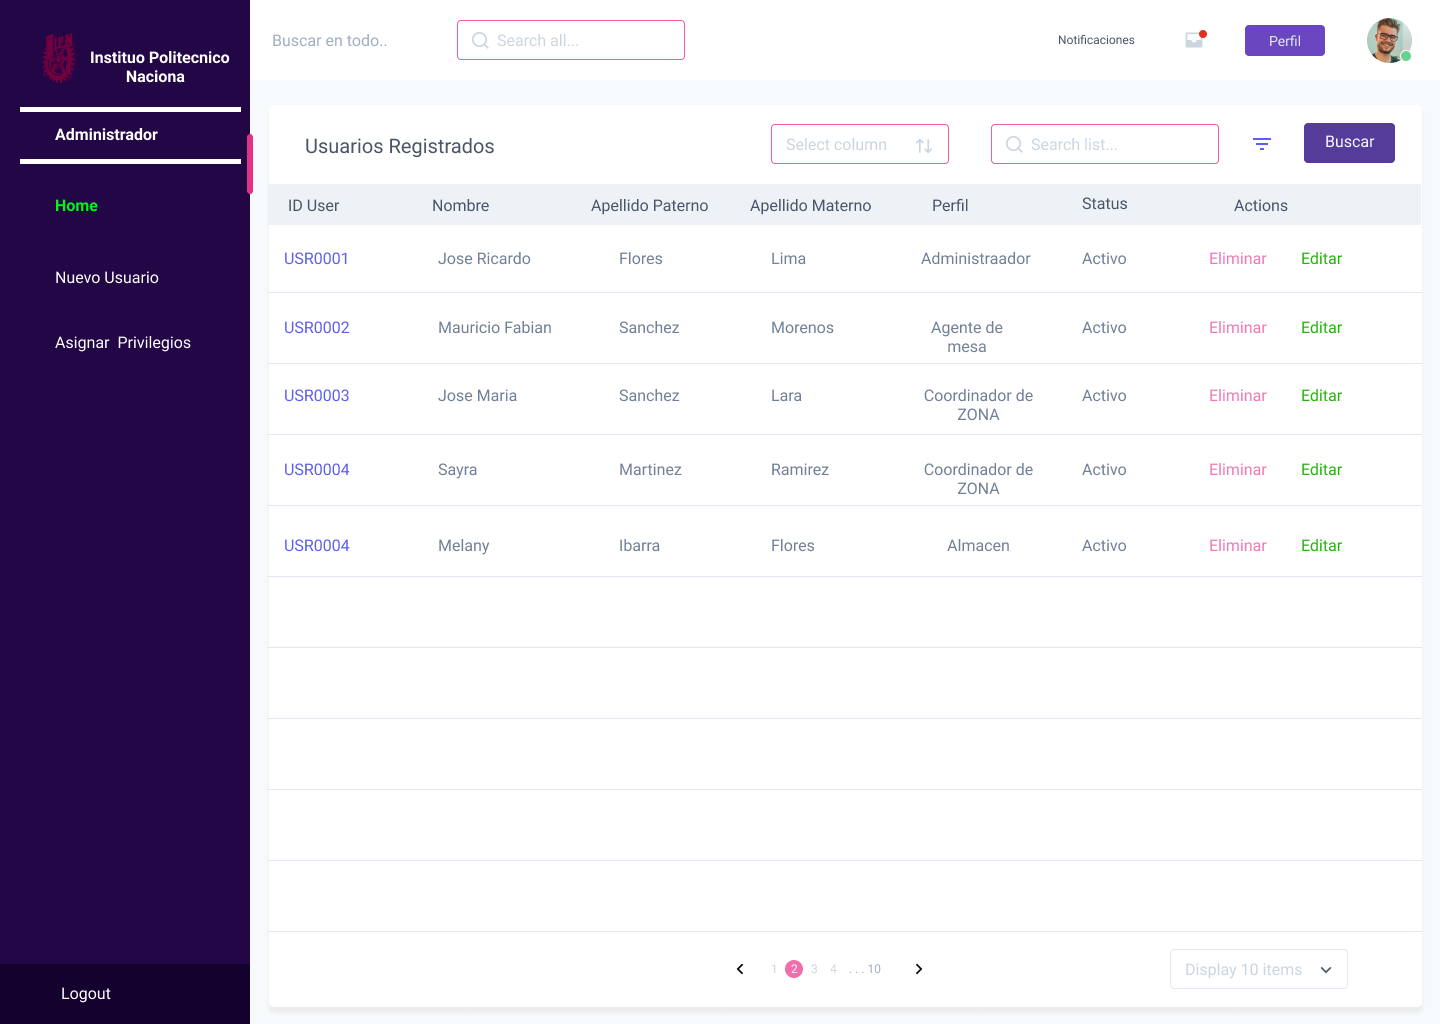
\includegraphics[width=0.75\textwidth]{Capitulo4/Img/GestionUser/Home-admin}
	\caption{Interfaz - home  administrador de sistema}
	\label{fig:INFHOMADMIN}
\end{figure}

En la interfaz home-admin se encuentran dos tipos de acciones principales, la primera infiere a eliminar el registro del usuario, solo es necesario seleccionar esta acción para que el sistema muestre una alerta de confirmación sobre la acción a realizar como se muestra en la interfaz \ref{fig:ELIMIAD}


\begin{figure}[H]
	\centering
	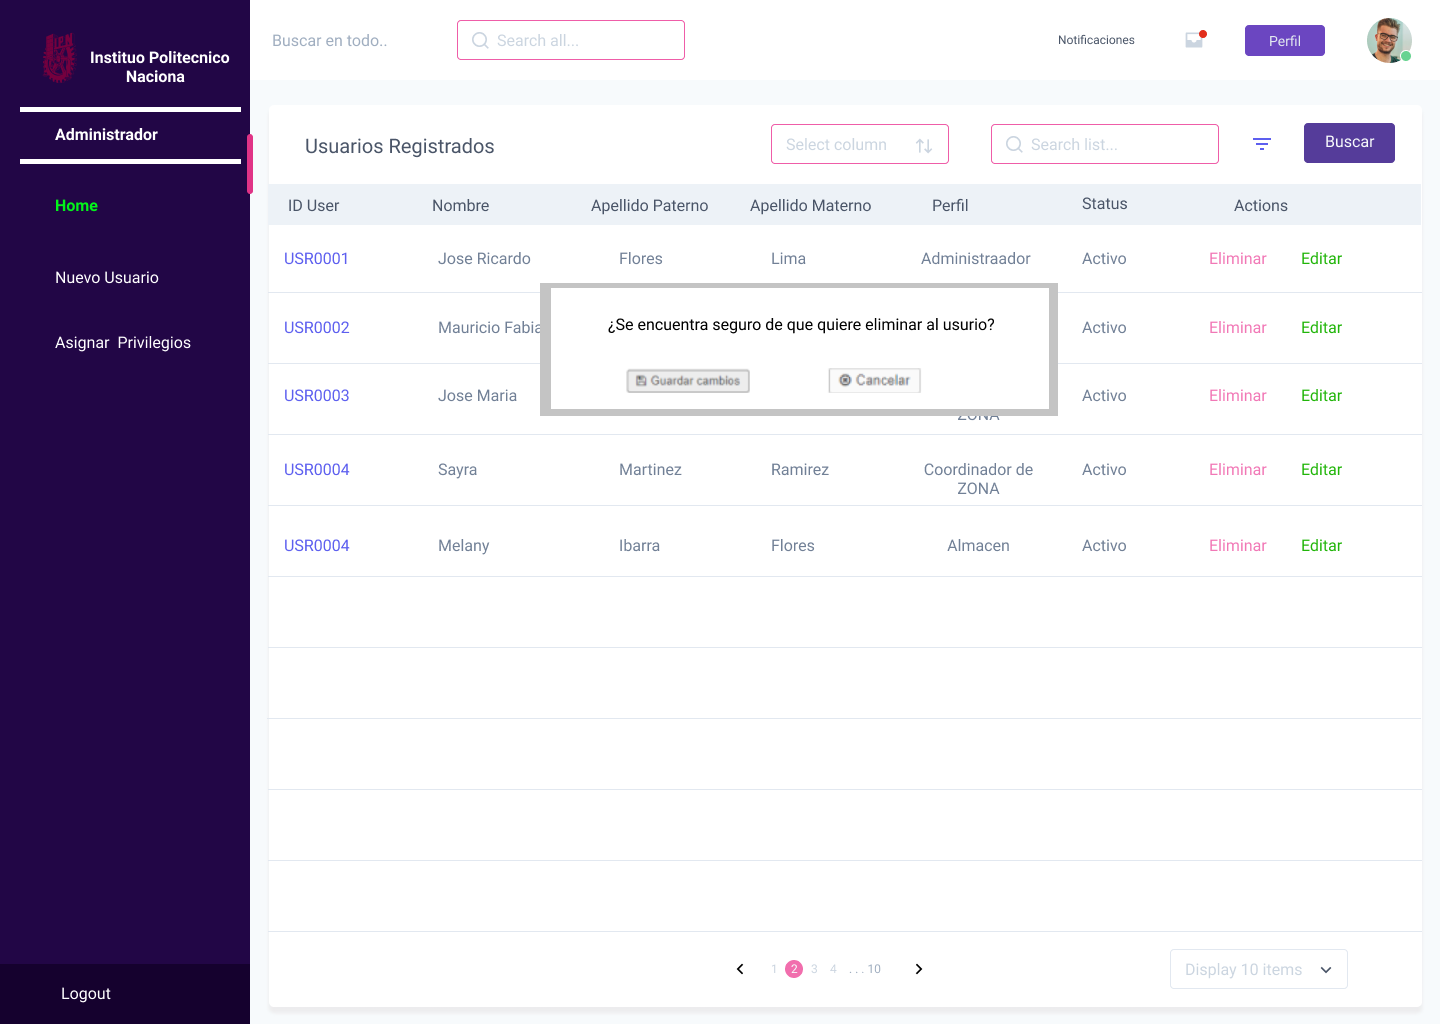
\includegraphics[width=0.75\textwidth]{Capitulo4/Img/GestionUser/Eliminar}
	\caption{Interfaz - Baja de usuario administrador }
	\label{fig:ELIMIAD}
\end{figure}


Como segunda acción en la interfaz de home-admin se presenta la  de "editar" donde desplegara una nueva interfaaz en la cual se mostrara la información del usuario, asi como la función de cambiar contraseña, como se muestra en la figura \ref{fig:ModADM}

\begin{figure}[H]
	\centering
	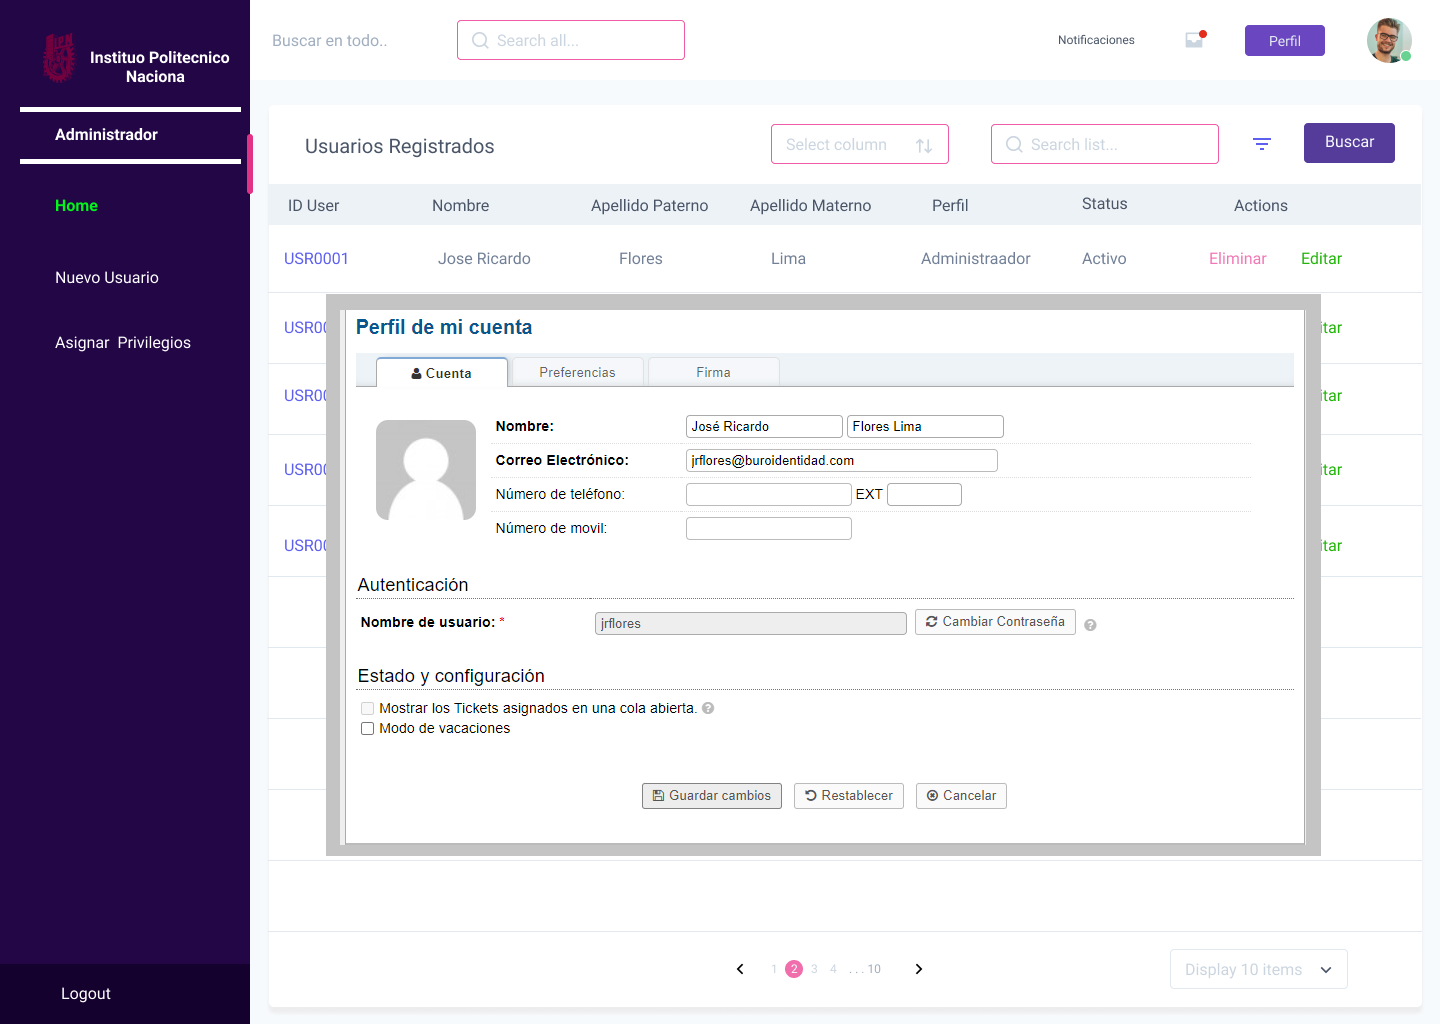
\includegraphics[width=0.75\textwidth]{Capitulo4/Img/GestionUser/Modificar_Datos}
	\caption{Interfaz -Modificación de datos de Usuarios}
	\label{fig:ModADM}
\end{figure}


Una de las acciones  del modulo de administración de usuario es el de dar de alta un nuevo usuario, por lo cual en la interfaz \ref{fig:Nievoadm} se describe un formulario que debe de llenar el administrador para el registro correcto de un nuevo usuario. 
\begin{figure}[H]
	\centering
	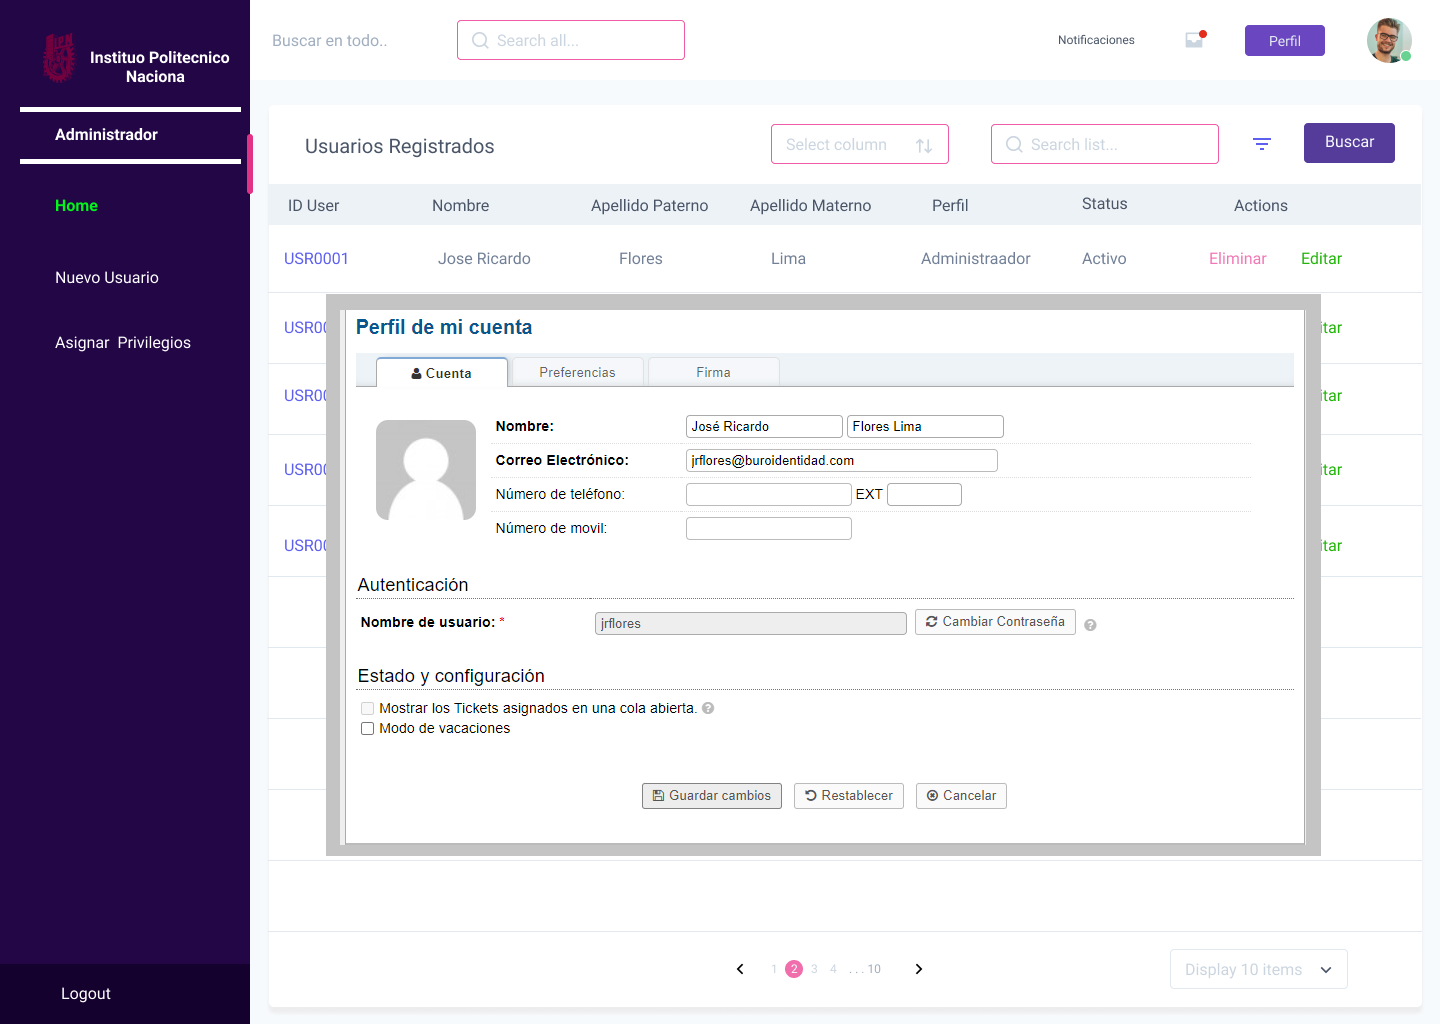
\includegraphics[width=0.75\textwidth]{Capitulo4/Img/GestionUser/Modificar_Datos}
	\caption{Interfaz - Nuevo usuario}
	\label{fig:Nievoadm}
\end{figure}


\newpage
\section{Diagrama de clases del sistema}

Dado que el paradigma de programación empleado en el desarrollo del proyecto es el de 
orientación a objetos, el diseño del sistema se ha realizado con una estructura de clases. 

A continuación se detallan las principales clases del sistemas mesa de servicio, figura \ref{fig:jbgsjkhdgb}. 
\begin{figure}[H]
	\centering
	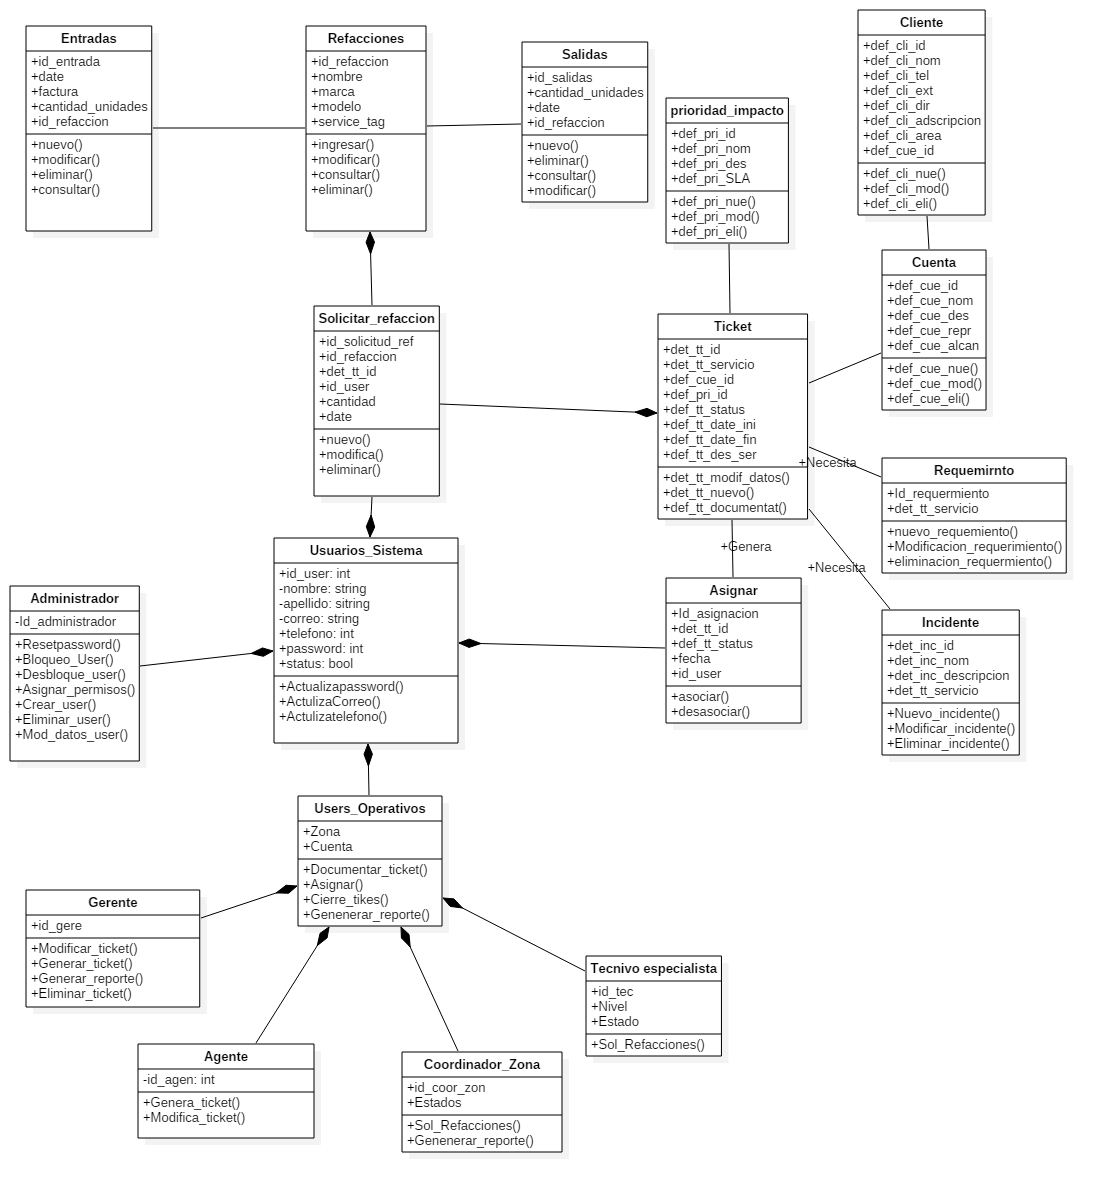
\includegraphics[width=0.95\textwidth]{Capitulo4/Diagramas/Completo}
	\caption{Diagrama de clases del sistema}
	\label{fig:jbgsjkhdgb}
\end{figure}

   % Table generated by Excel2LaTeX from sheet 'Hoja24'
 \begin{table}[H]
 	\centering
 	\caption{Descripcion de clase- Usuarios sistema}
 	\begin{tabular}{|r|r|}
 		\toprule
 		\rowcolor[rgb]{ .125,  .216,  .392} \multicolumn{2}{|p{34.215em}|}{\textcolor[rgb]{ 1,  1,  1}{\textbf{Clase Usuarios\_sistema}}} \\
 		\midrule
 		\multicolumn{1}{|p{6.145em}|}{\textbf{Clase}} & \multicolumn{1}{p{28.07em}|}{Usuarios\_Sistema} \\
 		\midrule
 		\multicolumn{1}{|p{6.145em}|}{\textbf{Descripción}} & \multicolumn{1}{p{28.07em}|}{Clase que representa la información de un usuario del sistema.} \\
 		\midrule
 		\multicolumn{1}{|p{6.145em}|}{\textbf{Atributos }} & \multicolumn{1}{p{28.07em}|}{•	Id\_user: identificador unívoco de usuario\newline{}•	Nombre: nombre de usuario\newline{}•	Apellidos: apellido de usuario \newline{}•	Correo: correo de usuario \newline{}•	Teléfono: numero de teléfono móvil de usuario\newline{}•	Password: contraseña para inicio de sesión en el sistema\newline{}•	Status: identifica si el usuario esta bloqueado o no. } \\
 		\midrule
 		\multicolumn{1}{|p{6.145em}|}{\textbf{Operaciones}} & \multicolumn{1}{p{28.07em}|}{•	Actualizapassword() :  método que realiza la actualización del password del usuario.\newline{}•	ActulizaCorreo(): método que realiza la actualización del correo personal del usuario.\newline{}•	Actulizatelefono() : método que realiza la actualización del numero de teléfono personal del usuario.} \\
 		\bottomrule
 	\end{tabular}%
 	\label{tab:CLAS1}%
 \end{table}%
 
 
   % Table generated by Excel2LaTeX from sheet 'Hoja24'
 \begin{table}[H]
 	\centering
 	\caption{Descripcion de clase-Administrador}
 	\begin{tabular}{|p{6.145em}|p{28.07em}|}
 		\toprule
 		\rowcolor[rgb]{ .125,  .216,  .392} \multicolumn{2}{|p{34.215em}|}{\textcolor[rgb]{ 1,  1,  1}{\textbf{Clase Administrador }}} \\
 		\midrule
 		\textbf{Clase} & \multicolumn{1}{l|}{Administrador } \\
 		\midrule
 		\textbf{Descripción} & Clase que representa la información y funciones que desarrolladora el usuario administrador. \\
 		\midrule
 		\textbf{Atributos } & •	Id\_administador: identificador unívoco de administrador \\
 		\midrule
 		\textbf{Operaciones} & •	Resetpassword() :  método que realiza el cambio del password a cualquier usuario del sistema.\newline{}•	Bloqueo\_User(): método que realiza el bloqueo del usuario en el sistema\newline{}•	Desbloqueo\_user() : método que realiza el desbloqueo del usuario en el sistema\newline{}•	Asignar\_permisos() : método que realiza la asignación, asi mismo la actualización de permisos y eliminación de estos.\newline{}•	Eliminar\_user(): método que realiza la eliminación de usuarios pertenecientes al sistemas \newline{}•	Mod\_datos\_user(): método que realiza la modificación de los datos con los que fueron enrolados los usuarios del sistema. \\
 		\bottomrule
 	\end{tabular}%
 	\label{tab:CLAS2}%
 \end{table}%
 
  % Table generated by Excel2LaTeX from sheet 'Hoja24'
\begin{table}[H]
	\centering
	\caption{Descripcion de clase-Agente}
	\begin{tabular}{|p{6.145em}|p{28.07em}|}
		\toprule
		\rowcolor[rgb]{ .125,  .216,  .392} \multicolumn{2}{|p{34.215em}|}{\textcolor[rgb]{ 1,  1,  1}{\textbf{Clase Agente  }}} \\
		\midrule
		\textbf{Clase} & \multicolumn{1}{l|}{Agente  } \\
		\midrule
		\textbf{Descripción} & Clase que representa la información  del usuario del sistema, agente de mesa de servicio  \\
		\midrule
		\textbf{Atributos } & •id\_agen: identificador único del agente de mesa de servicio \\
		\midrule
		\textbf{Operaciones} & •	Modificar\_ticket()  :  método que realiza la modificación de los datos asi como cualquier contenido que tenga el ticket\newline{}•	Generar\_ticket(): método que la creación de un ticket \\
		\bottomrule
	\end{tabular}%
	\label{tab:CLAS3}%
\end{table}%


  % Table generated by Excel2LaTeX from sheet 'Hoja24'
\begin{table}[htbp]
	\centering
	\caption{Descripcion de clase-Gerente}
	\begin{tabular}{|p{6.145em}|p{28.07em}|}
		\toprule
		\rowcolor[rgb]{ .125,  .216,  .392} \multicolumn{2}{|p{34.215em}|}{\textcolor[rgb]{ 1,  1,  1}{\textbf{Clase Gerente }}} \\
		\midrule
		\textbf{Clase} & \multicolumn{1}{l|}{Gerente } \\
		\midrule
		\textbf{Descripción} & Clase que representa la información del usuario gerente. \\
		\midrule
		\textbf{Atributos } & •	Id\_gere: identificador único del gerente. \\
		\midrule
		\textbf{Operaciones} & •	Modificar\_ticket()  :  método que realiza la modificación de los datos asi como cualquier contenido que tenga el ticket\newline{}•	Generar\_ticket(): método que la creación de un ticket\newline{}•	Generar\_reporte()  : método que realiza reportes generales de la operación de mesa de servicio\newline{}•	Eliminar\_ticket()  : método que realiza la eliminación de un ticket. \\
		\bottomrule
	\end{tabular}%
	\label{tab:clas4}%
\end{table}%


  % Table generated by Excel2LaTeX from sheet 'Hoja24'
\begin{table}[H]
	\centering
	\caption{Descripcion de clase-Coordinador\_Zona}
	\begin{tabular}{|p{6.145em}|p{28.07em}|}
		\toprule
		\rowcolor[rgb]{ .125,  .216,  .392} \multicolumn{2}{|p{34.215em}|}{\textcolor[rgb]{ 1,  1,  1}{\textbf{Clase Coordinador\_Zona }}} \\
		\midrule
		\textbf{Clase} & \multicolumn{1}{l|}{Coordinador\_Zona} \\
		\midrule
		\textbf{Descripción} & Clase que representa la información del usuario gerente. \\
		\midrule
		\textbf{Atributos } & •	id\_coor\_zon: identificador único del coordinador de zona de mesa de servicio\newline{}•	Estados:  identifica a los estados de la república que atiende el usuario coordinador de zona  \\
		\midrule
		\textbf{Operaciones} & •	Sol\_Refacciones()   :  método que realiza la solicitud de refacciones al almacén para la atención de tickets.\newline{}•	Genenerar\_reporte() : método que realiza reportes de atención de servicios por estado por región, y por técnico especialista a su cargo. \\
		\bottomrule
	\end{tabular}%
	\label{tab:clas5}%
\end{table}%

  % Table generated by Excel2LaTeX from sheet 'Hoja24'
\begin{table}[H]
	\centering
	\caption{Descripcion de clase-Técnico\_especialista}
	\begin{tabular}{|p{6.145em}|p{28.07em}|}
		\toprule
		\rowcolor[rgb]{ .125,  .216,  .392} \multicolumn{2}{|p{34.215em}|}{\textcolor[rgb]{ 1,  1,  1}{\textbf{Clase Técnico\_especialista}}} \\
		\midrule
		\textbf{Clase} & \multicolumn{1}{l|}{Técnico\_especialista} \\
		\midrule
		\textbf{Descripción} & Clase que representa la información del usuario del sistema, técnico especialista  \\
		\midrule
		\textbf{Atributos } & •	id\_tec identificador único del técnico especialista de mesa de servicio\newline{}•	Nivel: identifica el nivel de atención que puede generar el técnico especialista, Primero, según o tercer nivel\newline{}•	Estados:  identifica a la cobertura de estados donde puede atender el técnico especialista. \\
		\midrule
		\textbf{Operaciones} & •	Sol\_Refacciones()   :  método que realiza la solicitud de refacciones al almacén para la atención de tickets. \\
		\bottomrule
	\end{tabular}%
	\label{tab:clas6}%
\end{table}%



  % Table generated by Excel2LaTeX from sheet 'Hoja24'
\begin{table}[H]
	\centering
	\caption{Descripcion de clase-Asignar}
	\begin{tabular}{|p{6.145em}|p{28.07em}|}
		\toprule
		\rowcolor[rgb]{ .125,  .216,  .392} \multicolumn{2}{|p{34.215em}|}{\textcolor[rgb]{ 1,  1,  1}{\textbf{Clase Asignar}}} \\
		\midrule
		\textbf{Clase} & \multicolumn{1}{l|}{Asignar} \\
		\midrule
		\textbf{Descripción} & Clase que representa la información de las operaciones realizadas de asignación entre usuarios del sistema y el ticket  de atención del servicio. \\
		\midrule
		\textbf{Atributos } & •	Id\_asignacion: identifica el identificador único de transición de asignación \newline{}•	det\_tt\_id: identificador único de ticket.\newline{}•	def\_tt\_status: identifica el estatus del flujo del ticket.\newline{}•	Fecha: identifica la fecha y hora de transición de asignación \newline{}•	id\_user: identificador único de usuario \\
		\midrule
		\textbf{Operaciones} & •	asociar()   :  método que realiza la asociación de un ticket a un usuario del sistema.\newline{}•	desasociar()  : método que realiza la desasociación  de un ticket a un usuario del sistema. \\
		\bottomrule
	\end{tabular}%
	\label{tab:clas7}%
\end{table}%


  % Table generated by Excel2LaTeX from sheet 'Hoja24'
\begin{table}[H]
	\centering
	\caption{Descripcion de clase-Ticket}
	\begin{tabular}{|p{6.145em}|p{28.07em}|}
		\toprule
		\rowcolor[rgb]{ .125,  .216,  .392} \multicolumn{2}{|p{34.215em}|}{\textcolor[rgb]{ 1,  1,  1}{\textbf{Clase Ticket}}} \\
		\midrule
		\textbf{Clase} & \multicolumn{1}{l|}{Asignar} \\
		\midrule
		\textbf{Descripción} & Clase que representa la información del ticket. \\
		\midrule
		\textbf{Atributos } & •	det\_tt\_id: identificador único de ticket.\newline{}•	def\_tt\_status: identifica el estatus del flujo del ticket.\newline{}•	det\_tt\_servicio: identifica el tipo de servicio del ticket \newline{}•	def\_cue\_id: identifica la cuenta a la cual esta asociado el servicio del ticket \newline{}•	def\_pri\_id: identifica el nivel de prioridad asi como el nivel de SLA \newline{}•	def\_tt\_status: identifica el estatus del flujo del ticket.\newline{}•	def\_tt\_date\_ini: identifica la fecha y hora de creación de ticket. \newline{}•	def\_tt\_date\_fin: identifica la fecha y hora de cierre de ticket\newline{}•	def\_tt\_des\_ser: identifica la descripción de la solicitud del servicio, error a solucionar.  \\
		\midrule
		\textbf{Operaciones} & •	det\_tt\_modif\_datos() :  método que realiza la modificación de la información contenida en el ticket. \newline{}•	det\_tt\_nuevo() : método que realiza la creación de un ticket\newline{}•	def\_tt\_documentat()   : método que realiza la generación de un hilo de atención sobre la atención. \\
		\bottomrule
	\end{tabular}%
	\label{tab:clas8}%
\end{table}%



  % Table generated by Excel2LaTeX from sheet 'Hoja24'
	\begin{table}[H]
	\centering
	\caption{Descripcion de clase-Users\_Operativos}
	\begin{tabular}{|p{6.145em}|p{28.07em}|}
		\toprule
		\rowcolor[rgb]{ .125,  .216,  .392} \multicolumn{2}{|p{34.215em}|}{\textcolor[rgb]{ 1,  1,  1}{\textbf{Clase Users\_Operativos}}} \\
		\midrule
		\textbf{Clase} & \multicolumn{1}{l|}{Users\_Operativos} \\
		\midrule
		\textbf{Descripción} & Clase que representa la información de los usuarios con categoría de operativos \\
		\midrule
		\textbf{Atributos } & •	Zona: idéntica la zona de atención que tendrá el usuario operativo. \newline{}•	Cuenta\_asi: identifica los clientes en cuentas que tendrá asignados para la atención el usuario operativo. \\
		\midrule
		\textbf{Operaciones} & •	Documentar\_ticket()   :  método que realiza la creación de un hilo de comentarios sobre el seguimiento del ticket.\newline{}•	Asignar() : método que  realiza la reasignación del ticket a algún perteneciente al flujo del ticket.\newline{}•	Cierre\_tikes(): método que realiza el cierre de un ticket.\newline{}•	Generar\_reporte()  : método que realiza reportes generales de la operación de mesa de servicio. \\
		\bottomrule
	\end{tabular}%
	\label{tab:clas9}%
\end{table}%


  % Table generated by Excel2LaTeX from sheet 'Hoja24'
\begin{table}[H]
	\centering
	\caption{Descripcion de clase-Incidente}
	\begin{tabular}{|p{6.145em}|p{28.07em}|}
		\toprule
		\rowcolor[rgb]{ .125,  .216,  .392} \multicolumn{2}{|p{34.215em}|}{\textcolor[rgb]{ 1,  1,  1}{\textbf{Clase  Incidente}}} \\
		\midrule
		\textbf{Clase} & \multicolumn{1}{l|}{Incidente} \\
		\midrule
		\textbf{Descripción} & Clase que representa la información de los servicios clasificados como incidentes. \\
		\midrule
		\textbf{Atributos } & •	det\_inc\_id: identificador unico de incidente.\newline{}•	det\_inc\_nom: identifica el nombre del incidente.\newline{}•	det\_inc\_descripcion: identifica la descripción a detalle del incidente.\newline{}•	det\_tt\_servicio: identifica el tipo de servicio del ticket  \\
		\midrule
		\textbf{Operaciones} & •	Nuevo\_incidente()   :  método que realiza la creación de un nuevo requerimiento.\newline{}•	Modificar\_incidente()  : método que  realiza la modificación de información del incidente.\newline{}•	Eliminar\_incidente() : método que realiza la eliminación de un incidente. \\
		\bottomrule
	\end{tabular}%
	\label{tab:CLAS10}%
\end{table}%


  % Table generated by Excel2LaTeX from sheet 'Hoja24'
\begin{table}[H]
	\centering
	\caption{Descripcion de clase-Requerimiento}
	\begin{tabular}{|p{6.145em}|p{28.07em}|}
		\toprule
		\rowcolor[rgb]{ .125,  .216,  .392} \multicolumn{2}{|p{34.215em}|}{\textcolor[rgb]{ 1,  1,  1}{\textbf{Clase Requerimiento}}} \\
		\midrule
		\textbf{Clase} & \multicolumn{1}{l|}{Requerimiento} \\
		\midrule
		\textbf{Descripción} & Clase que representa la información de los servicios clasificados como requerimientos. \\
		\midrule
		\textbf{Atributos } & •	det\_req\_id: identificador único de requerimiento.\newline{}•	det\_req\_nom: identifica el nombre del requerimiento.\newline{}•	det\_req\_descripcion: identifica la descripción a detalle del requerimiento.\newline{}•	det\_tt\_servicio: identifica el tipo de servicio del ticket  \\
		\midrule
		\textbf{Operaciones} & •	Nuevo\_requerimiento()   :  método que realiza la creación de un nuevo requerimiento.\newline{}•	Modificar\_requerimiento()  : método que  realiza la modificación de información del requerimiento.\newline{}•	Eliminar\_requerimiento() : método que realiza la eliminación de un requerimiento. \\
		\bottomrule
	\end{tabular}%
	\label{tab:CLAS11}%
\end{table}%


  % Table generated by Excel2LaTeX from sheet 'Hoja24'
\begin{table}[H]
	\centering
	\caption{Descripcion de clase-Cuenta}
	\begin{tabular}{|p{6.145em}|p{28.07em}|}
		\toprule
		\rowcolor[rgb]{ .125,  .216,  .392} \multicolumn{2}{|p{34.215em}|}{\textcolor[rgb]{ 1,  1,  1}{\textbf{Clase Cuenta}}} \\
		\midrule
		\textbf{Clase} & \multicolumn{1}{l|}{Cuenta} \\
		\midrule
		\textbf{Descripción} & Clase que representa la información de los servicios clasificados como cuentas o clientes registrados para darles servicio. \\
		\midrule
		\textbf{Atributos } & •	def\_cue\_id: identificador unico de cuenta.\newline{}•	def\_cue \_nom: identifica el nombre de la cuenta.\newline{}•	def\_cue \_desc: identifica la descripción a detalle de la cuenta.\newline{}•	def\_cue\_rep: identifica la persona responsable directa de la cuenta, apoderado de la cuenta.\newline{}•	def\_cue\_alcan: identifica el alcance de la cuenta, regional, nacional, o estatal. \\
		\midrule
		\textbf{Operaciones} & •	def\_cue\_nue():  método que realiza la creación de un nuevo cuenta.\newline{}•	def\_cue\_mod(): método que  realiza la modificación de información del cuenta.\newline{}•	def\_cue\_eli(): método que realiza la eliminación de un cuenta. \\
		\bottomrule
	\end{tabular}%
	\label{tab:CLass12}%
\end{table}%


  % Table generated by Excel2LaTeX from sheet 'Hoja24'
\begin{table}[H]
	\centering
	\caption{Descripcion de clase-Prioridad\_ impacto}
	\begin{tabular}{|p{6.145em}|p{28.07em}|}
		\toprule
		\rowcolor[rgb]{ .125,  .216,  .392} \multicolumn{2}{|p{34.215em}|}{\textcolor[rgb]{ 1,  1,  1}{\textbf{Clase Prioridad\_impacto}}} \\
		\midrule
		\textbf{Clase} & \multicolumn{1}{l|}{Prioridad\_ impacto} \\
		\midrule
		\textbf{Descripción} & Clase que representa la información de prioridad e impacto. \\
		\midrule
		\textbf{Atributos } & •	def\_pri \_id: identificador único de Prioridad e impacto.\newline{}•	def\_pri\_nom: identifica el nombre del Prioridad e impacto.\newline{}•	def\_pri\_desc: identifica la descripción a detalle del Prioridad e impacto.\newline{}•	def\_pri\_SLA: identifica el nivel de atención de SLA \\
		\midrule
		\textbf{Operaciones} & •	def\_pri\_nue():  método que realiza la creación de un nuevo criterio de prioridad.\newline{}•	def\_pri\_mod(): método que  realiza la modificación de información de la  prioridad.\newline{}•	def\_pri\_eli(): método que realiza la eliminación de una Prioridad. \\
		\bottomrule
	\end{tabular}%
	\label{tab:clas13}%
\end{table}%


  % Table generated by Excel2LaTeX from sheet 'Hoja24'
\begin{table}[H]
	\centering
	\caption{Descripcion de clase-Refacciones}
	\begin{tabular}{|p{6.145em}|p{28.07em}|}
		\toprule
		\rowcolor[rgb]{ .125,  .216,  .392} \multicolumn{2}{|p{34.215em}|}{\textcolor[rgb]{ 1,  1,  1}{\textbf{Clase Refacciones}}} \\
		\midrule
		\textbf{Clase} & \multicolumn{1}{l|}{Refacciones} \\
		\midrule
		\textbf{Descripción} & Clase que representa la información de las refacciones en almacén  \\
		\midrule
		\textbf{Atributos } & •	id\_refaccion: identificador único de refacción.\newline{}•	nombre: identifica el nombre de la refacción.\newline{}•	marca: identifica la marca de la refacción.\newline{}•	modelo: identifica el modelo de la refacción.\newline{}•	Date: fecha y hora en que se genera la solicitud.\newline{}•	service\_tag: identifica el numero de serie de la refacción \\
		\midrule
		\textbf{Operaciones} & •	ingresar() :  método que realiza la creación de una alta de una nueva refacción.\newline{}•	modifica() : método que  realiza la modificación de información de la refacción.\newline{}•	eliminar() : método que realiza la eliminación de una refacción.\newline{}•	Consulta() : consulta la información del registro de la información. \\
		\bottomrule
	\end{tabular}%
	\label{tab:class14}%
\end{table}%


  % Table generated by Excel2LaTeX from sheet 'Hoja24'
\begin{table}[H]
	\centering
	\caption{Descripcion de clase-Solicitar\_refaccion}
	\begin{tabular}{|p{6.145em}|p{28.07em}|}
		\toprule
		\rowcolor[rgb]{ .125,  .216,  .392} \multicolumn{2}{|p{34.215em}|}{\textcolor[rgb]{ 1,  1,  1}{\textbf{Clase Solicitar\_refaccion}}} \\
		\midrule
		\textbf{Clase} & \multicolumn{1}{l|}{Solicitar\_refaccion} \\
		\midrule
		\textbf{Descripción} & Clase que representa la información del proceso de solicitud de refacciones para la atención de un servicio. \\
		\midrule
		\textbf{Atributos } & •	id\_solicitud\_ref: identificador único de solicitud de refacción.\newline{}•	id\_refaccion: identificador único de refacción.\newline{}•	det\_tt\_id: identificador único de ticket.\newline{}•	id\_user: identificador único de usuario.\newline{}•	Cantidad: identifica la cantidad de refacciones del mismo tipo a solicitar.\newline{}•	Date: fecha y hora en que se genera la solicitud. \\
		\midrule
		\textbf{Operaciones} & •	nuevo() :  método que realiza la creación de una nueva solicitud de refacción.\newline{}•	modifica(): método que  realiza la modificación de información de la solicitud de refacción.\newline{}•	eliminar(): método que realiza la eliminación de una solicitud. \\
		\bottomrule
	\end{tabular}%
	\label{tab:clas15}%
\end{table}%


  % Table generated by Excel2LaTeX from sheet 'Hoja24'
\begin{table}[H]
	\centering
	\caption{Descripcion de clase-Entrada}
	\begin{tabular}{|p{6.145em}|p{28.07em}|}
		\toprule
		\rowcolor[rgb]{ .125,  .216,  .392} \multicolumn{2}{|p{34.215em}|}{\textcolor[rgb]{ 1,  1,  1}{\textbf{Clase Entrada }}} \\
		\midrule
		\textbf{Clase} & \multicolumn{1}{l|}{Entrada } \\
		\midrule
		\textbf{Descripción} & Clase que representa la información de las transacciones realizadas de nuevas refacciones entrantes al sistema de almacenes.  \\
		\midrule
		\textbf{Atributos } & •	id\_refaccion: identificador único de refacción.\newline{}•	id\_entrada: identificador único de transacción de entrada \newline{}•	factura: numero de factura asociada al ingreso de refacciones.\newline{}•	cantidad\_unidades: identifica la cantidad de refacciones a ingresar.\newline{}•	Date: fecha y hora en que se genera la entrada. \\
		\midrule
		\textbf{Operaciones} & •	nuevo()  :  método que realiza la creación de una alta de un ingreso de  refacciones.\newline{}•	modifica() : método que  realiza la modificación de información del ingreso de refacción.\newline{}•	eliminar() : método que realiza la eliminación de un ingreso de refacciones.\newline{}•	Consulta() : consulta la información del registro de ingreso de refacciones. \\
		\bottomrule
	\end{tabular}%
	\label{tab:class16}%
\end{table}%


  % Table generated by Excel2LaTeX from sheet 'Hoja24'
\begin{table}[H]
	\centering
	\caption{Descripcion de clase-Salidas}
	\begin{tabular}{|p{6.145em}|p{28.07em}|}
		\toprule
		\rowcolor[rgb]{ .125,  .216,  .392} \multicolumn{2}{|p{34.215em}|}{\textcolor[rgb]{ 1,  1,  1}{\textbf{Clase Salidas  }}} \\
		\midrule
		\textbf{Clase} & \multicolumn{1}{l|}{Salidas  } \\
		\midrule
		\textbf{Descripción} & Clase que representa la información de las transacciones realizadas de salidas de refacciones asignadas a servicios.  \\
		\midrule
		\textbf{Atributos } & •	id\_refaccion: identificador único de refacción.\newline{}•	id\_salidas: identificador único de transacción de salida \newline{}•	cantidad\_unidades: identifica la cantidad de refacciones a ingresar.\newline{}•	Date: fecha y hora en que se genera la entrada. \\
		\midrule
		\textbf{Operaciones} & •	nuevo()  :  método que realiza la creación de una salida asignada a un ticket.\newline{}•	modifica() : método que  realiza la modificación de información de salida de una transacción de asignación a un ticket .\newline{}•	eliminar() : método que realiza la eliminación de una salida..\newline{}•	Consulta() : consulta la información del registro de salida de refacciones. \\
		\bottomrule
	\end{tabular}%
	\label{tab:class17}%
\end{table}%


  % Table generated by Excel2LaTeX from sheet 'Hoja24'
\begin{table}[H]
	\centering
	\caption{Descripcion de clase-Cliente}
	\begin{tabular}{|p{6.145em}|p{28.07em}|}
		\toprule
		\rowcolor[rgb]{ .125,  .216,  .392} \multicolumn{2}{|p{34.215em}|}{\textcolor[rgb]{ 1,  1,  1}{\textbf{Clase Cliente   }}} \\
		\midrule
		\textbf{Clase} & \multicolumn{1}{l|}{Cliente   } \\
		\midrule
		\textbf{Descripción} & Clase que representa la información del cliente solicitante del servicio perteneciente a una cuenta registrada.  \\
		\midrule
		\textbf{Atributos } & •	def\_cli\_id: identificador único de cliente.\newline{}•	def\_cli\_nom: identifica el nombre completo del cliente.\newline{}•	def\_cli\_tel : identififica el teléfono del fijo o móvil del cliente.\newline{}•	def\_cli\_ext : identifica la extensión de comunicación telefónica.\newline{}•	def\_cli\_dir : identifica la la dirección del inmueble donde labora el cliente.\newline{}•	def\_cli\_adscripcion: identifica al departamento al que pertenece el cliente.\newline{}•	def\_cli\_area: identifica al área dentro del departamento al que pertenece el cliente.\newline{}•	def\_cue\_id: identificador único de cuenta.da. \\
		\midrule
		\textbf{Operaciones} & •	nuevo()  :  método que realiza la creación de un nuevo cliente.\newline{}•	modifica() : método que  realiza la modificación de información del cliente registrado.\newline{}•	eliminar() : método que realiza la eliminación de un cliente. \\
		\bottomrule
	\end{tabular}%
	\label{tab:class18}%
\end{table}%

\newpage
\section{Diagrama de Base de datos}
El modelo relacional es un modelo de datos lógico que representa la transformación del 
diseño conceptual y su normalización para realizar un diseño físico de la base de datos, ver figura \ref{fig:BDGENRAL}. 


\begin{figure}[H]
	\centering
	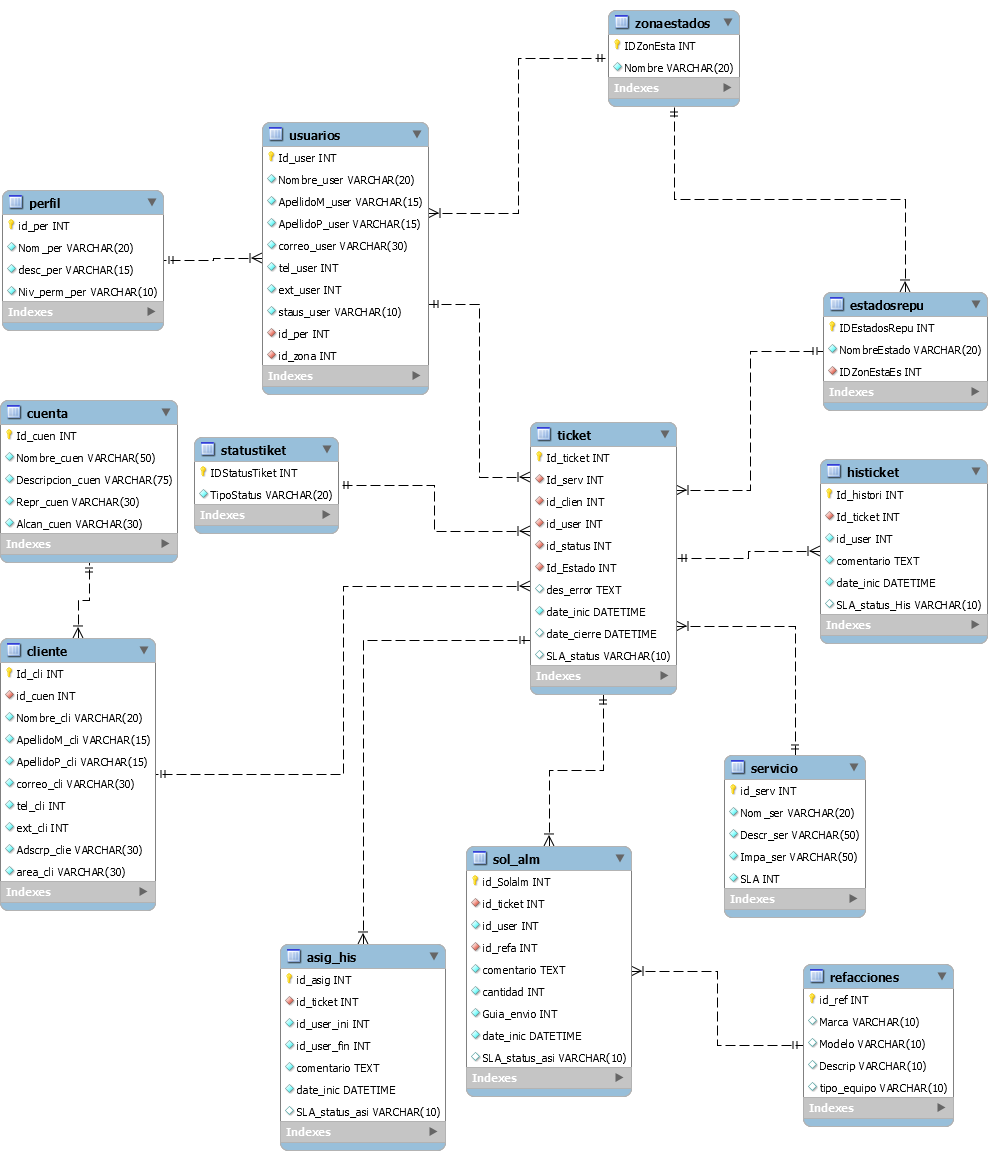
\includegraphics[width=0.95\textwidth]{Capitulo4/Diagramas/BaseDatos}
	\caption{Diagrama de base de datos}
	\label{fig:BDGENRAL}
\end{figure}
